\chapter{Form factors} \label{appendixff}

Table~\ref{tab:formfactors} lists the particles shapes whose form
factors have been implemented in \BornAgain.

\begin{table}[H] 
\caption{Table of form factors implemented in \BornAgain.} \label{tab:formfactors}
  \begin{tabulary} {0.95\textwidth}{Lc Lc L} 
\hline 
Shape & &   Shape& &   Shape \\
\hline 
Box,\SecRef{Box} & & Prism3, \SecRef{Prism3} & & Tetrahedron, \SecRef{Tetrahedron}  \\
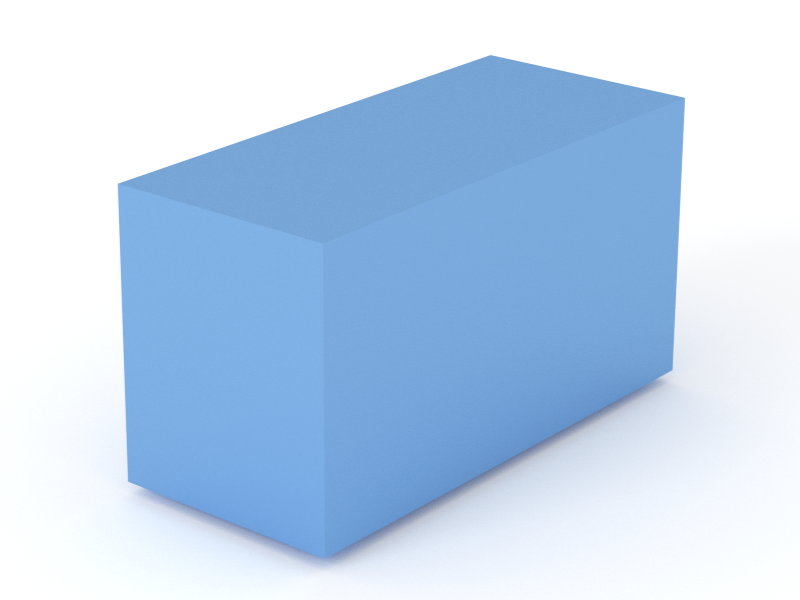
\includegraphics[width=1in]{Figures/Box3d} &
 & 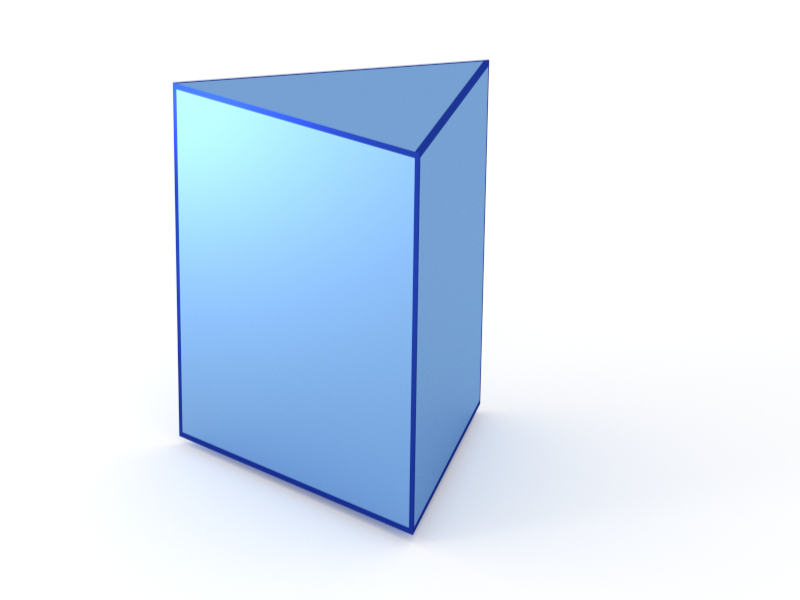
\includegraphics[width=1in]{Figures/Prism33d} & & 
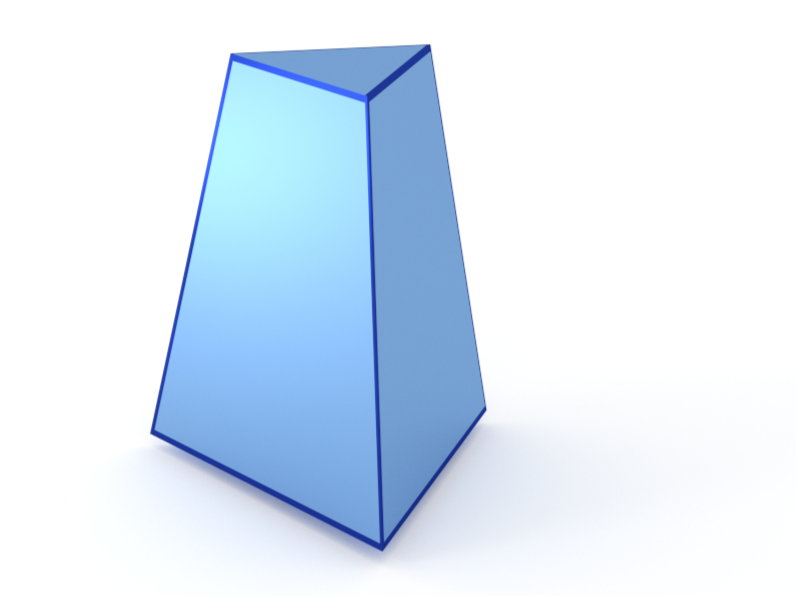
\includegraphics[width=1in]{Figures/Tetrahedron3d}
\\
\hline 
Prism6, \SecRef{Prism6}    & & Cone6, \SecRef{Cone6}  & &  Pyramid, \SecRef{Pyramid} \\
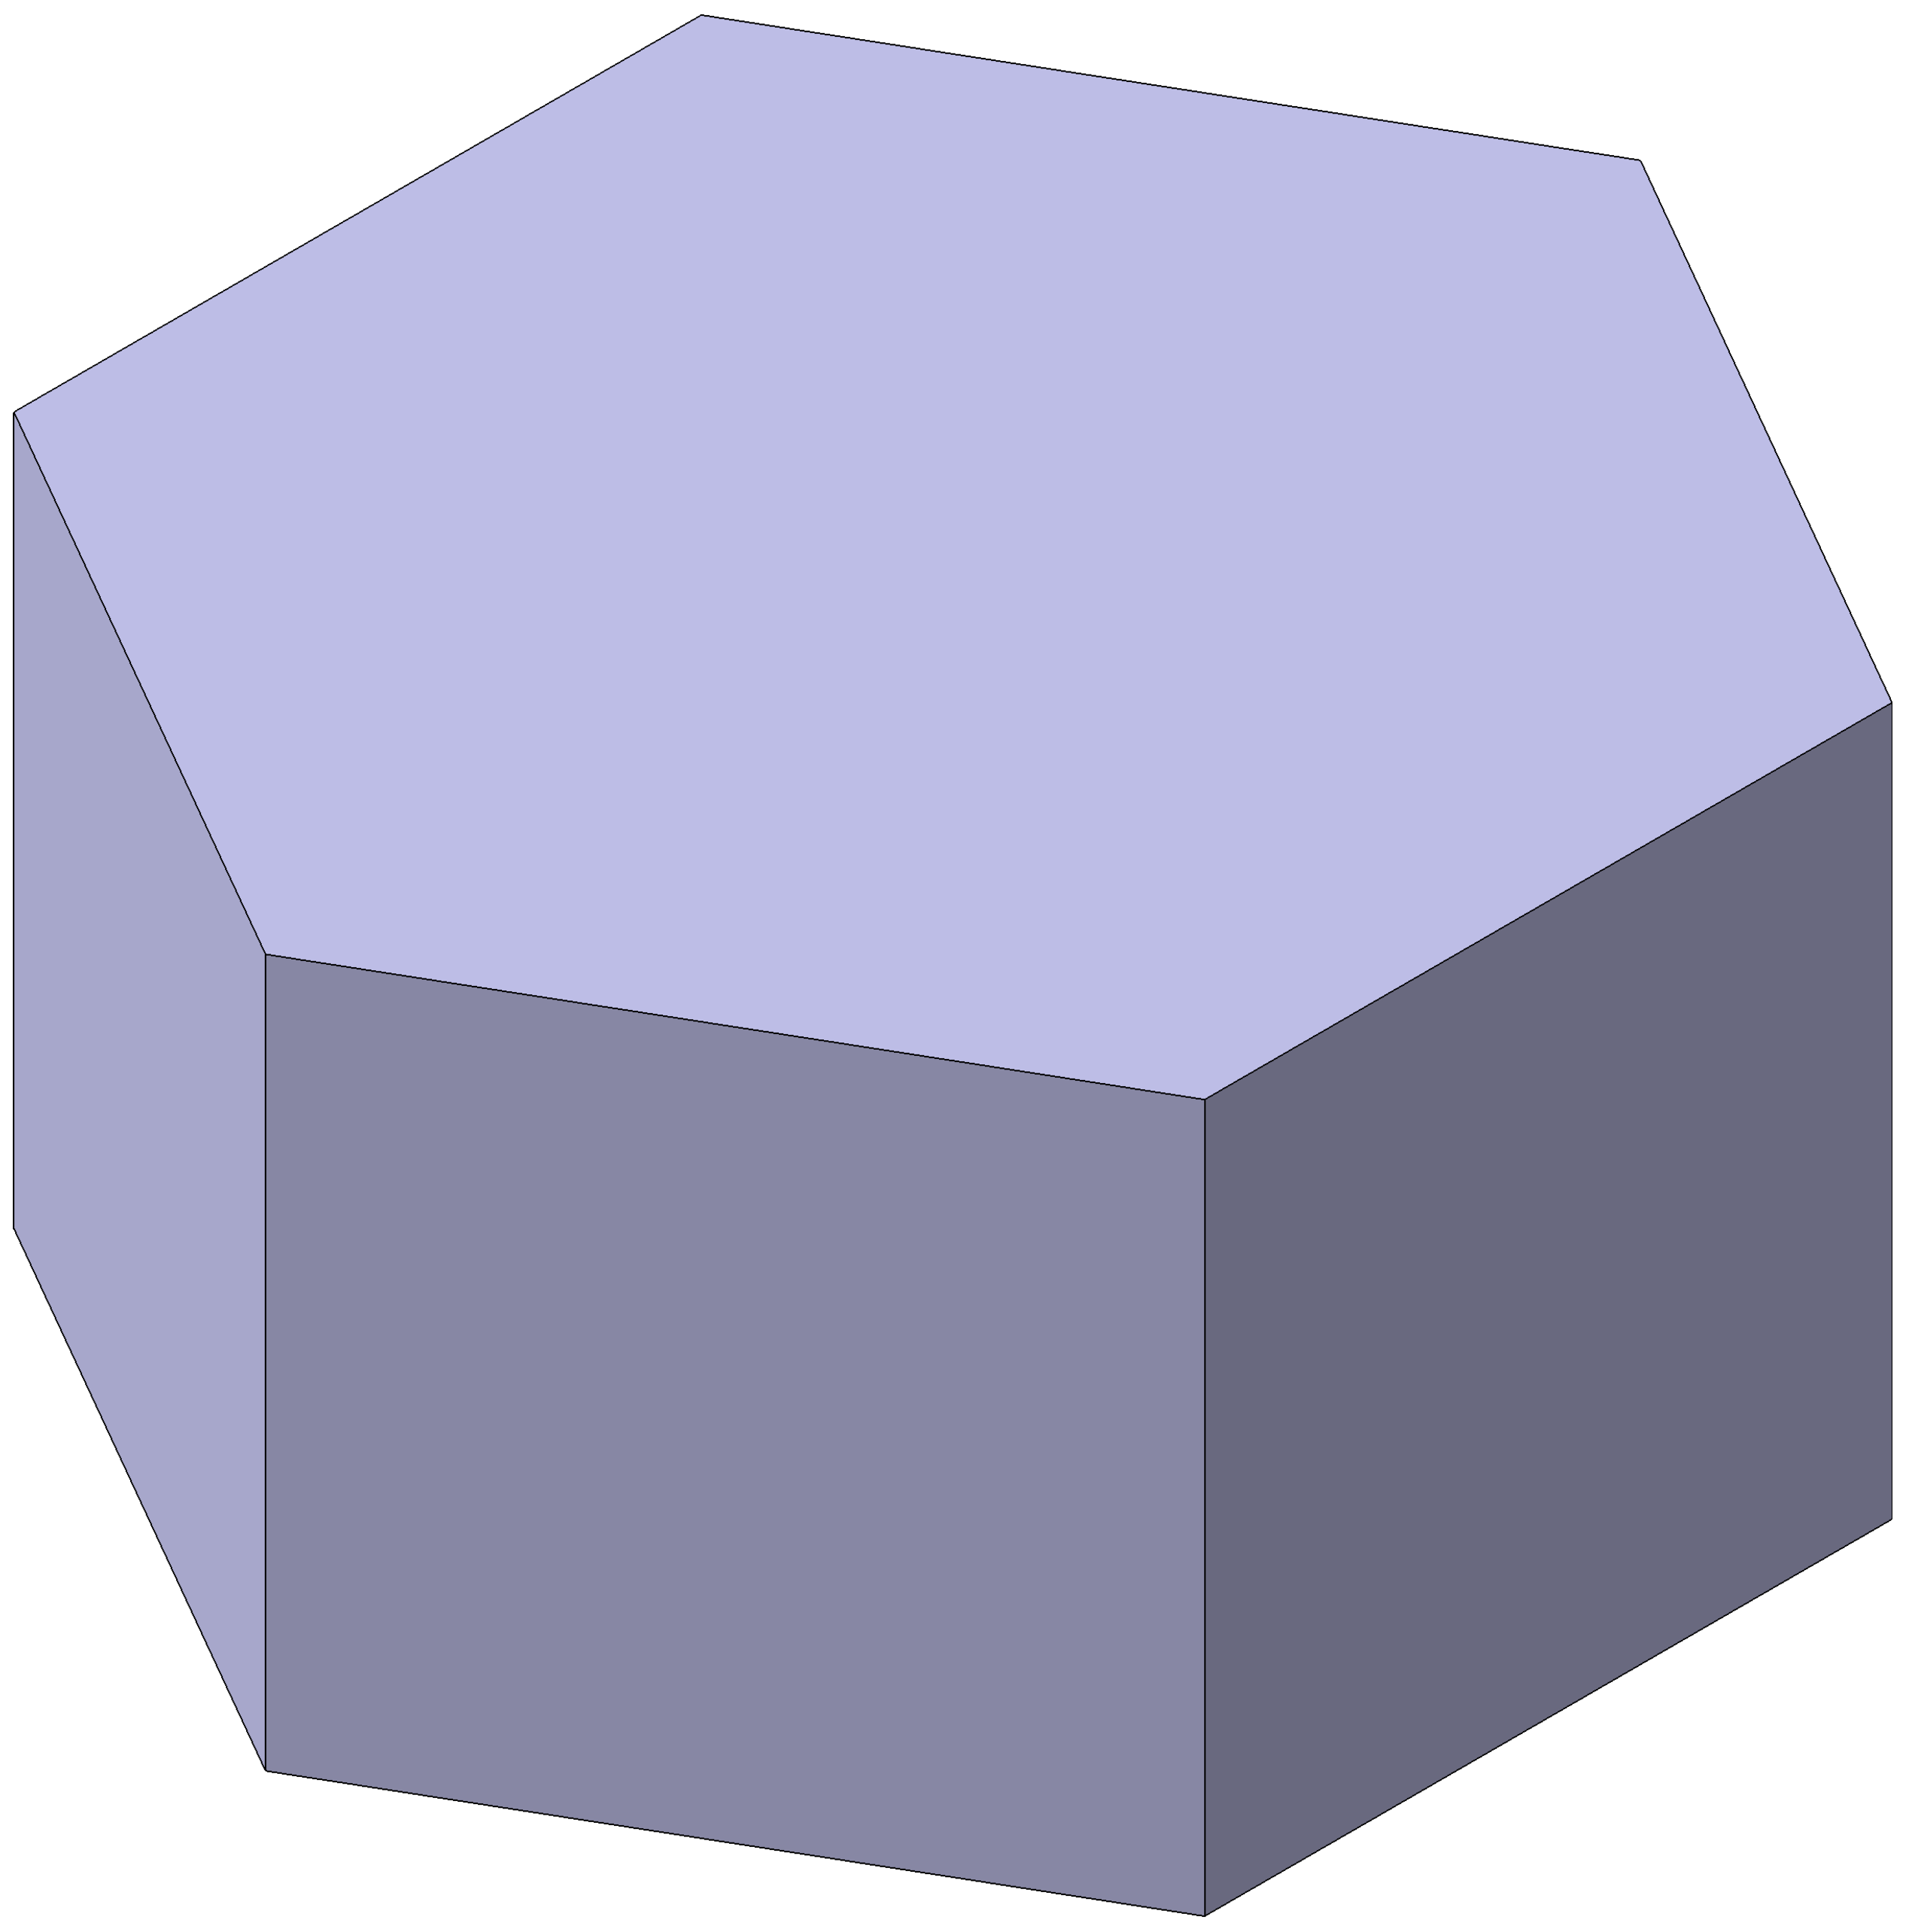
\includegraphics[width=1in]{Figures/Prism63d} & & 
 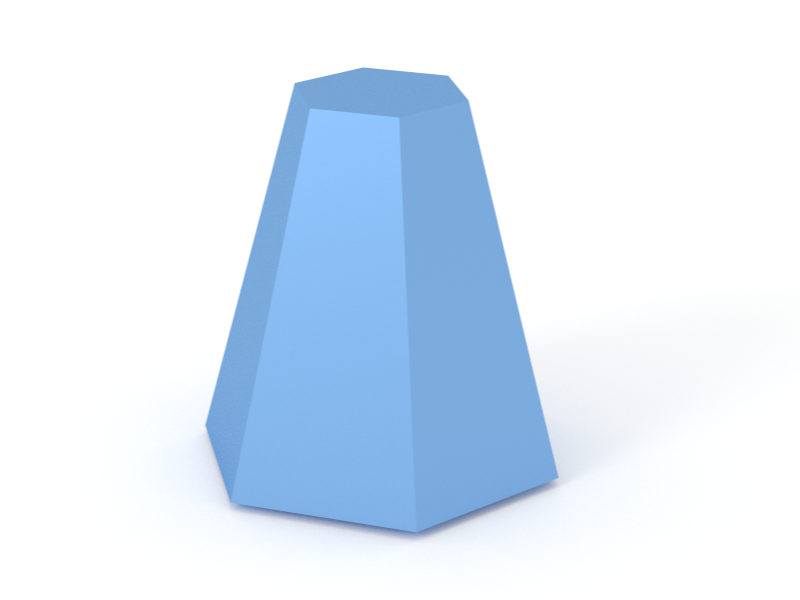
\includegraphics[width=1in]{Figures/Cone63d}  & & 
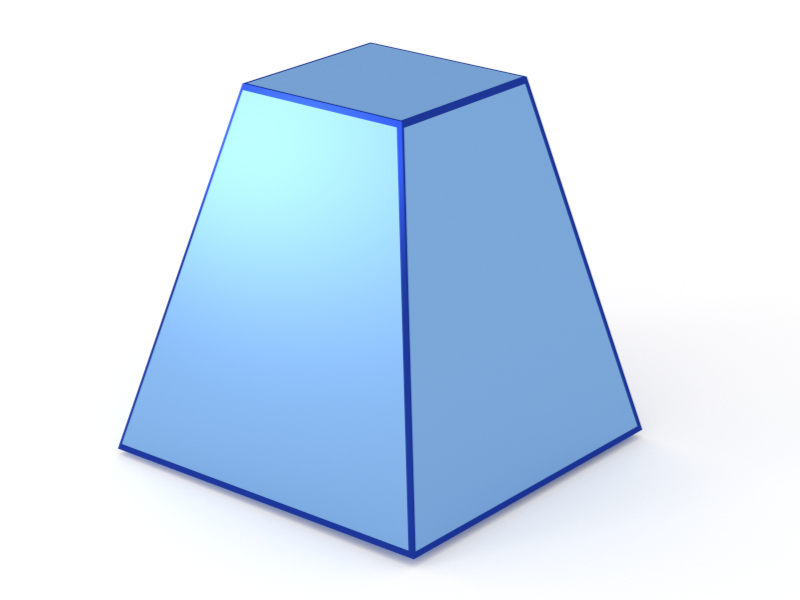
\includegraphics[width=1in]{Figures/Pyramid3d}
\\
\hline
 Anisotropic pyramid, \SecRef{AnisoPyramid} & &  Cuboctahedron,
 \SecRef{Cuboctahedron} & &   Cylinder, \SecRef{Cylinder} \\
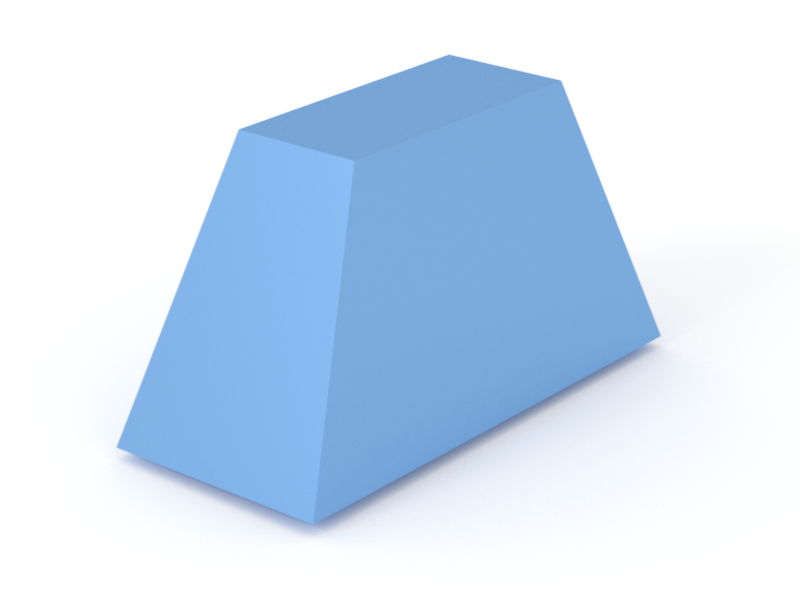
\includegraphics[width=1in]{Figures/AnistropicPyramid3d} &
    & 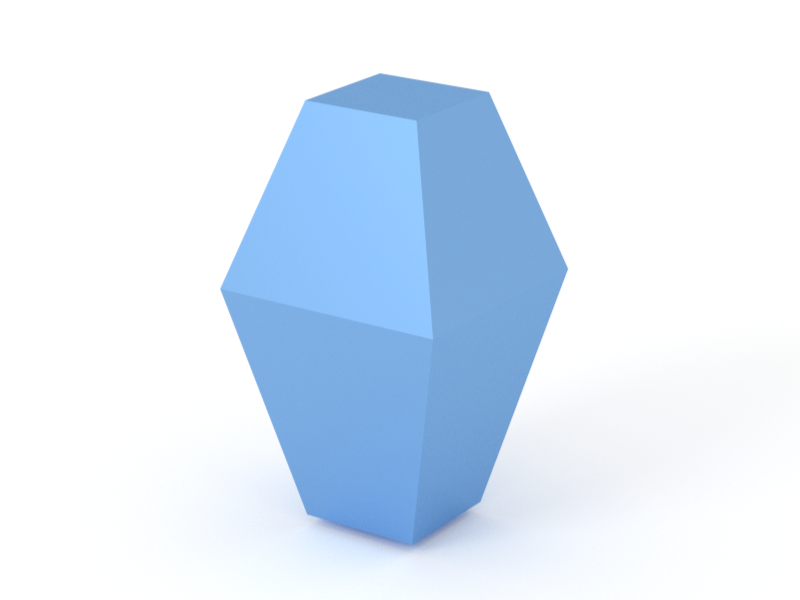
\includegraphics[width=1in]{Figures/Cuboctahedron3d} & & 
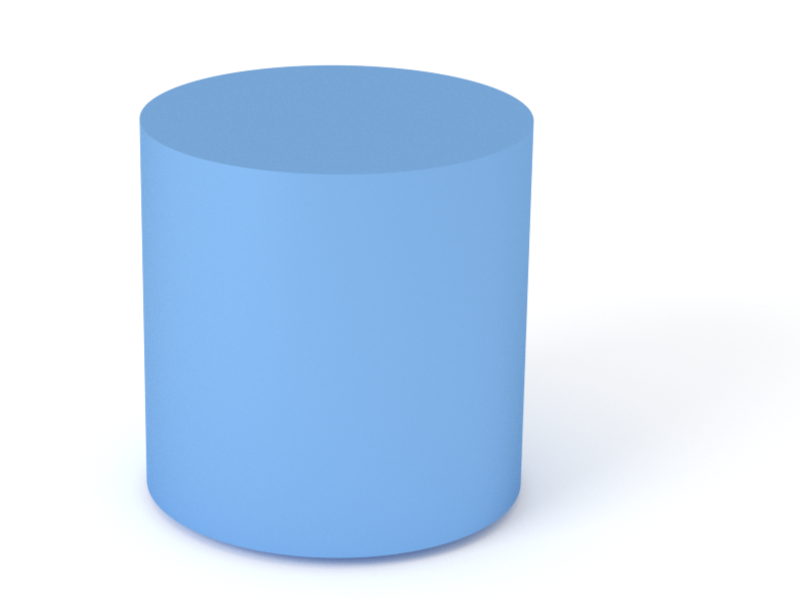
\includegraphics[width=1in]{Figures/Cylinder3d}\\
\hline
\end{tabulary}
\end{table}


\begin{table}[H] 
 \begin{tabulary} {0.95\textwidth}{Lc Lc L} 
\hline 
Shape & &   Shape & &   Shape \\
\hline
Ellipsoidal cylinder, \SecRef{EllipsoidalCylinder}  & &  Cone,
\SecRef{Cone} & & Full Sphere, \SecRef{FullSphere}  \\
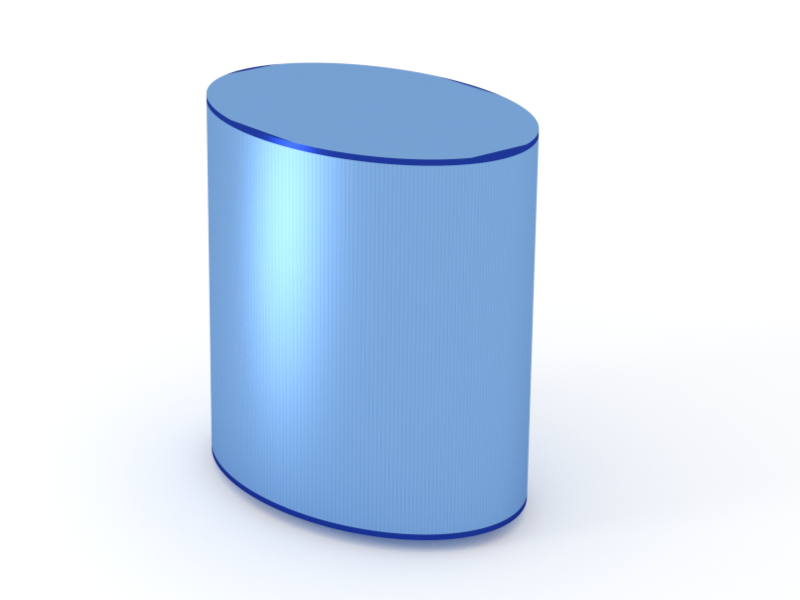
\includegraphics[width=1in]{Figures/EllipsoidalCylinder3d} &
& 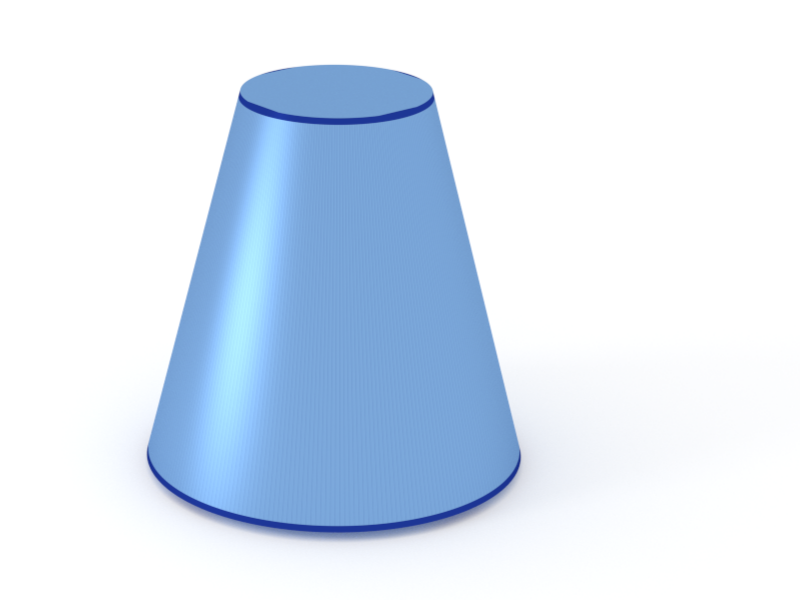
\includegraphics[width=1in]{Figures/Cone3d}
& & 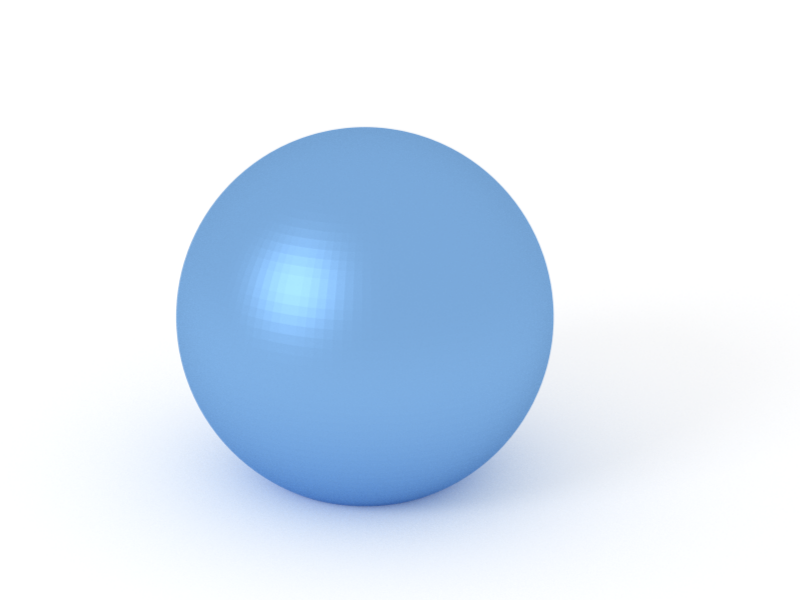
\includegraphics[width=1in]{Figures/FullSphere3d} \\
\hline
Truncated Sphere, \SecRef{Sphere}  & & Full Spheroid,
\SecRef{FullSpheroid} & & Truncated Spheroid, \SecRef{Spheroid} \\
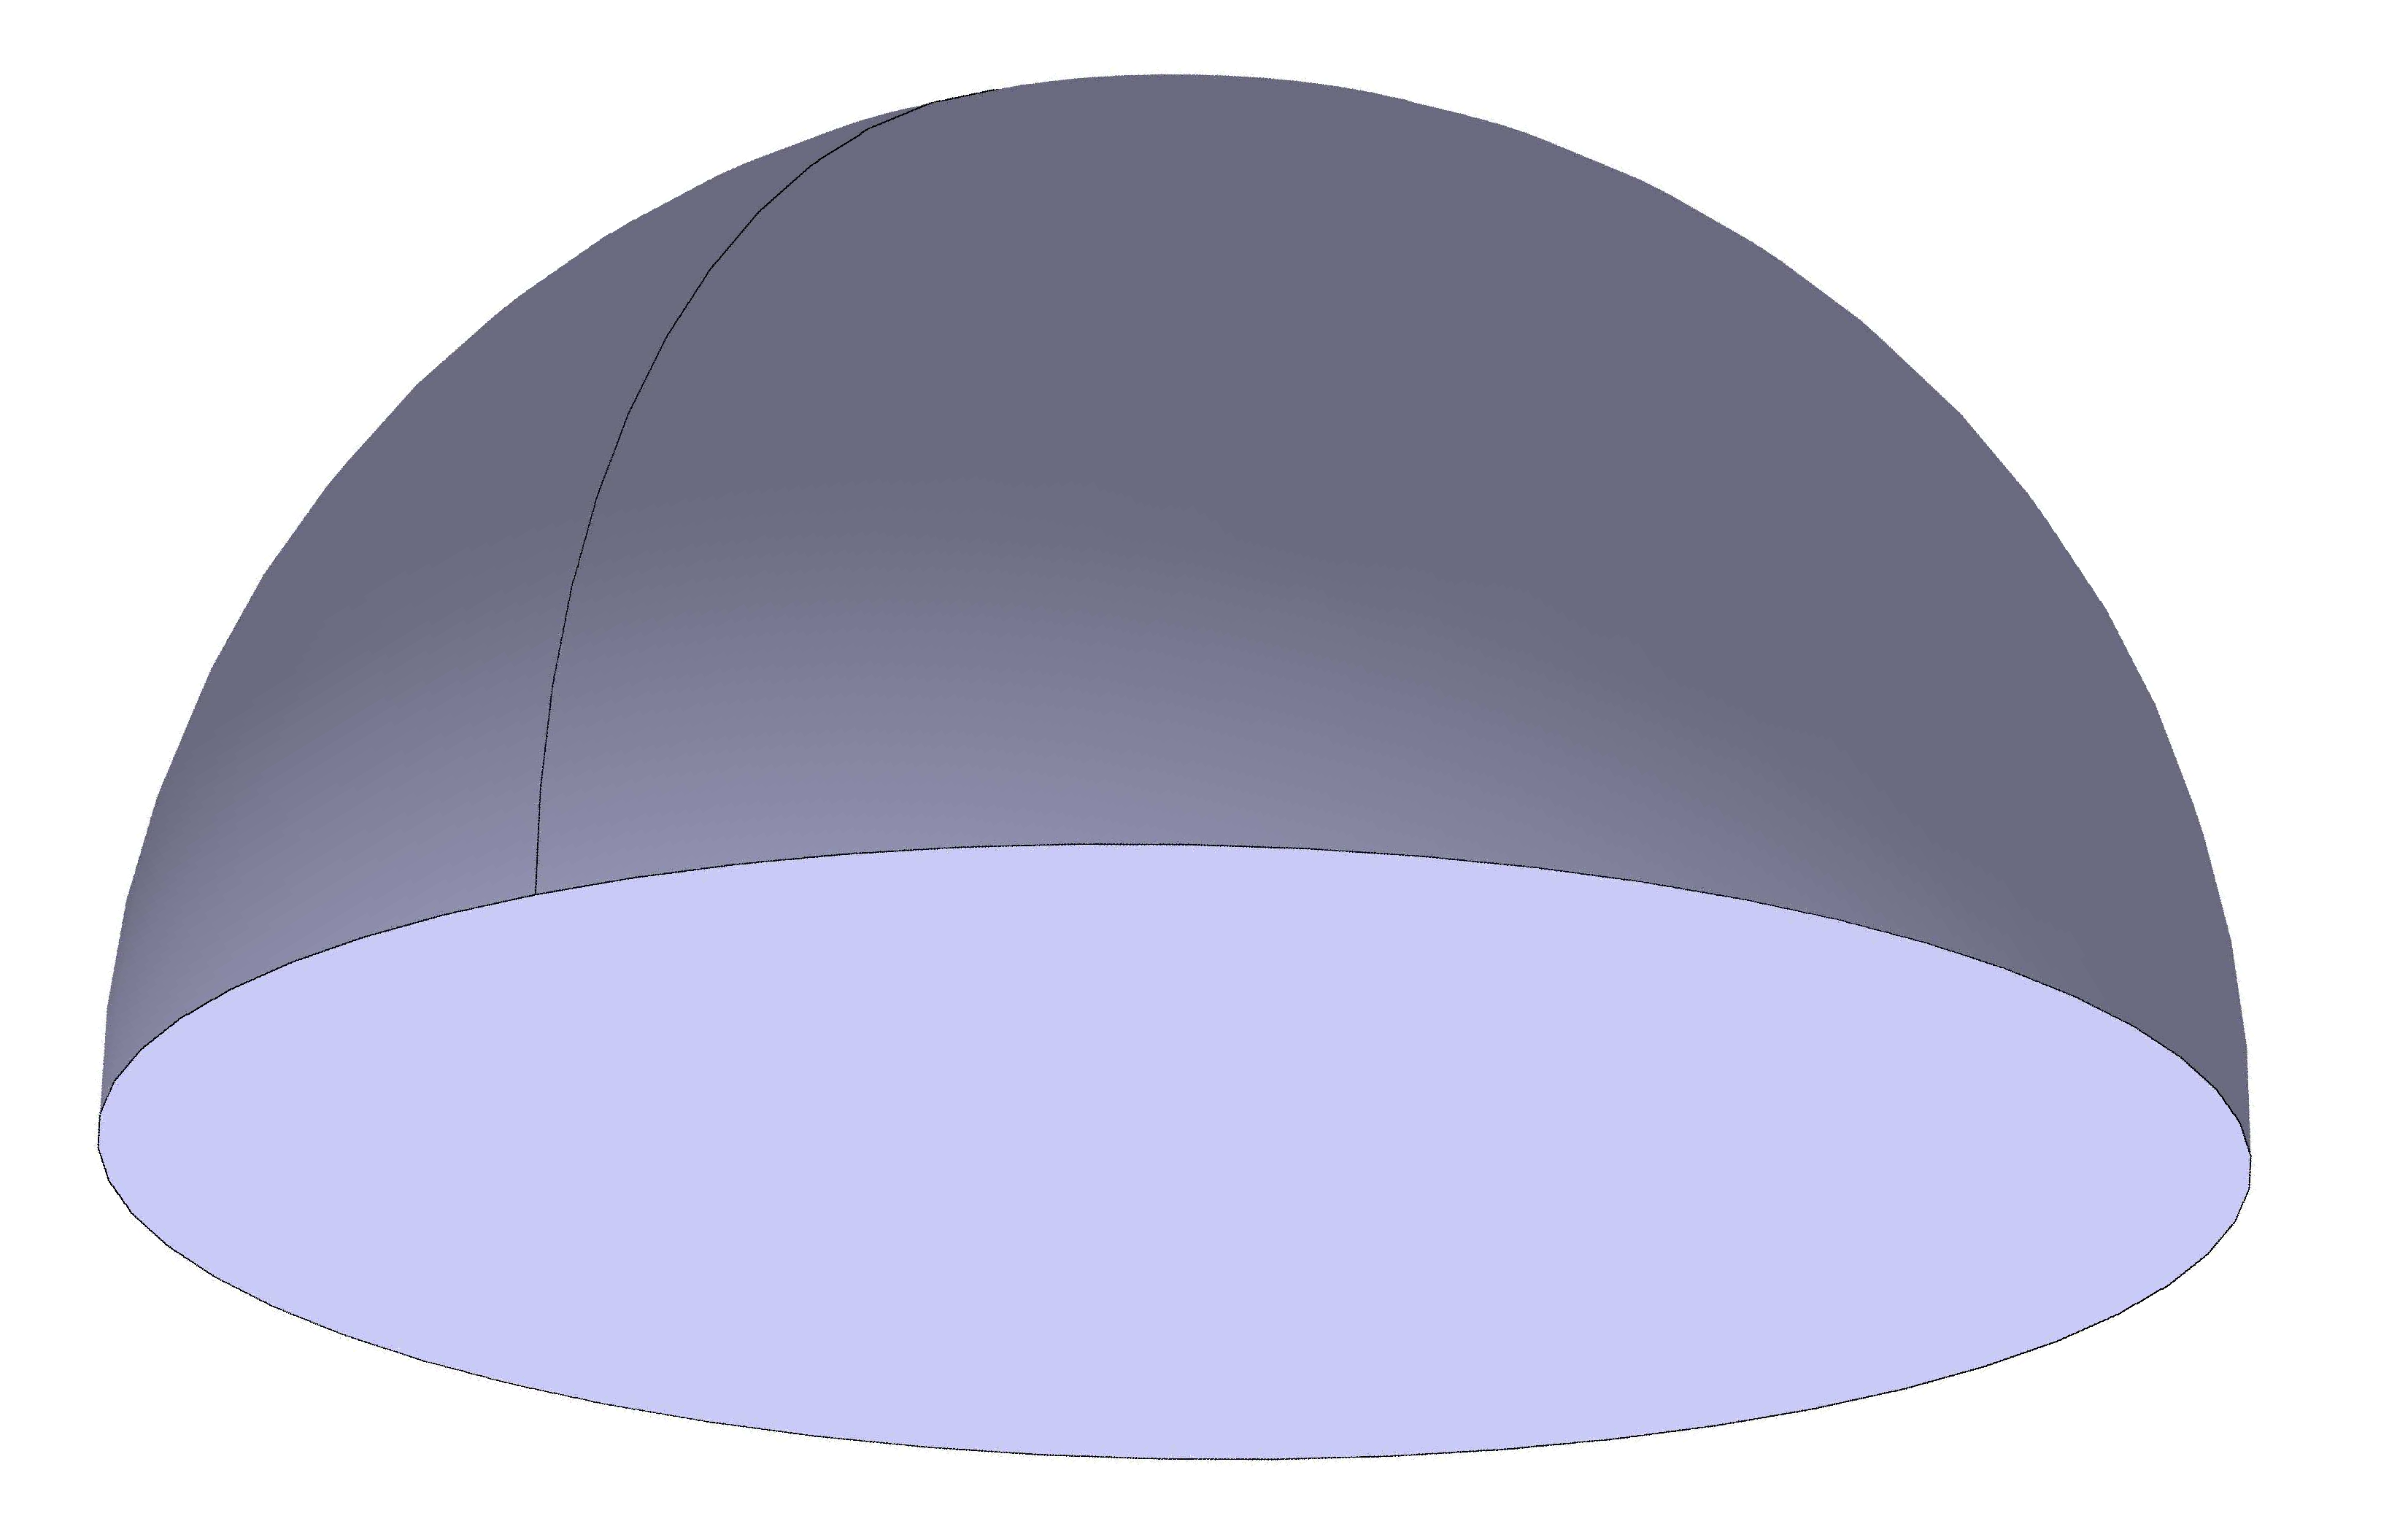
\includegraphics[width=1in]{Figures/Sphere3d} & &
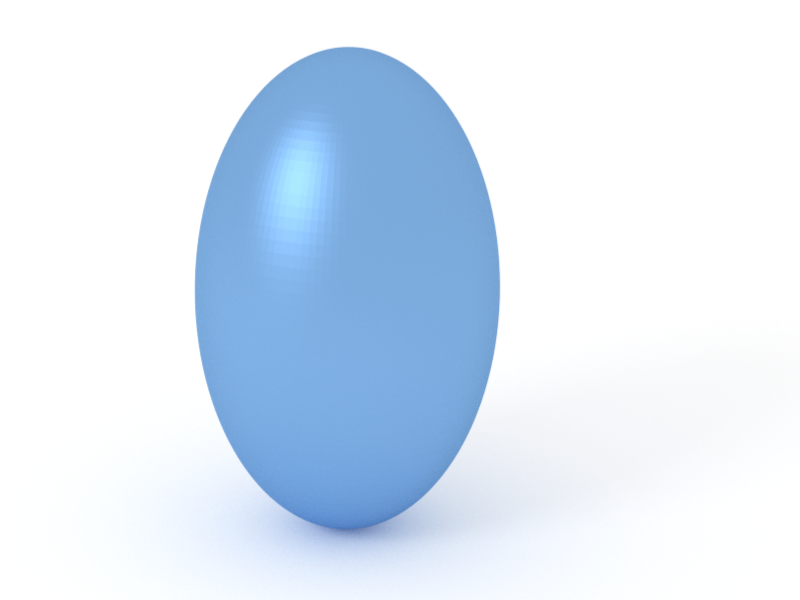
\includegraphics[width=1in]{Figures/FullSpheroid3d} & & 
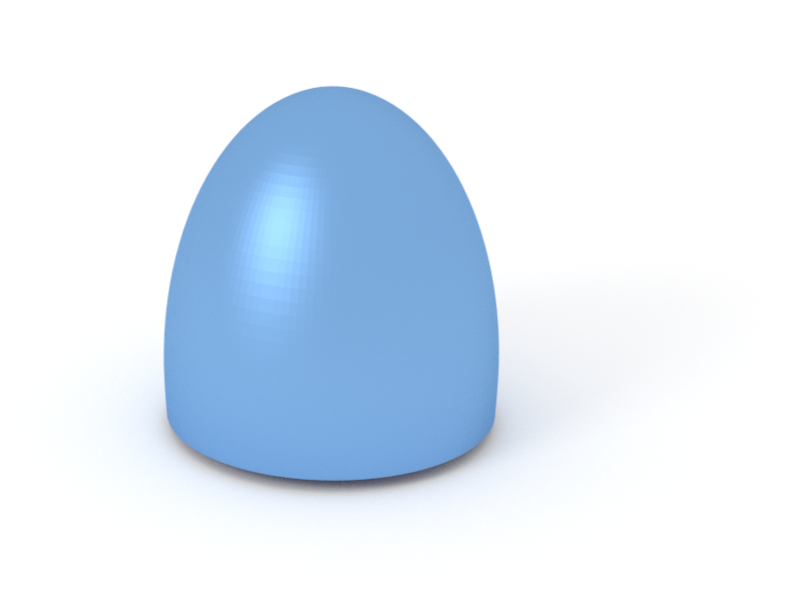
\includegraphics[width=1in]{Figures/Spheroid3d} \\
\hline 
 Hemi Ellipsoid, \SecRef{HemiEllipsoid}   & & Ripple1, \SecRef{Ripple1}   &  & Ripple2, \SecRef{Ripple2}   \\
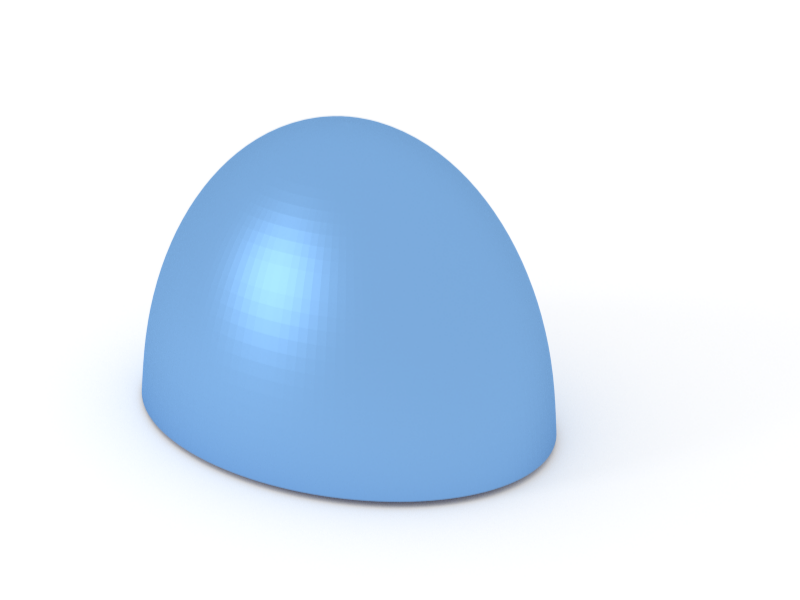
\includegraphics[width=1in]{Figures/HemiEllipsoid3d} & &
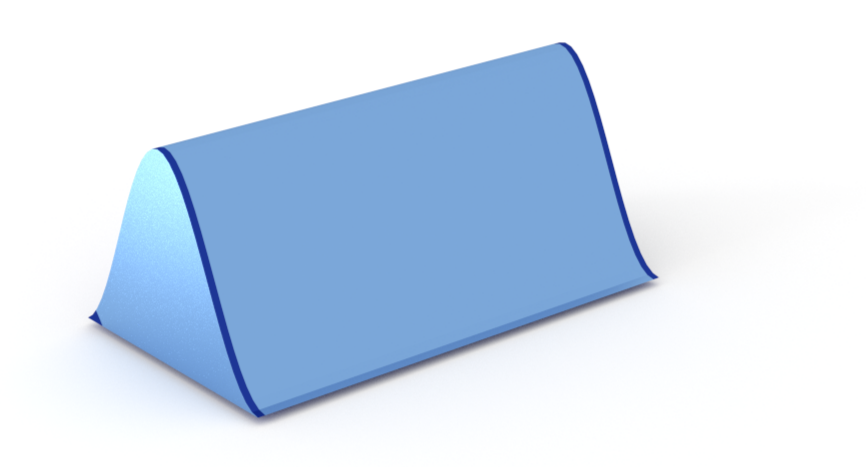
\includegraphics[width=1in]{Figures/Ripple13d} &
& 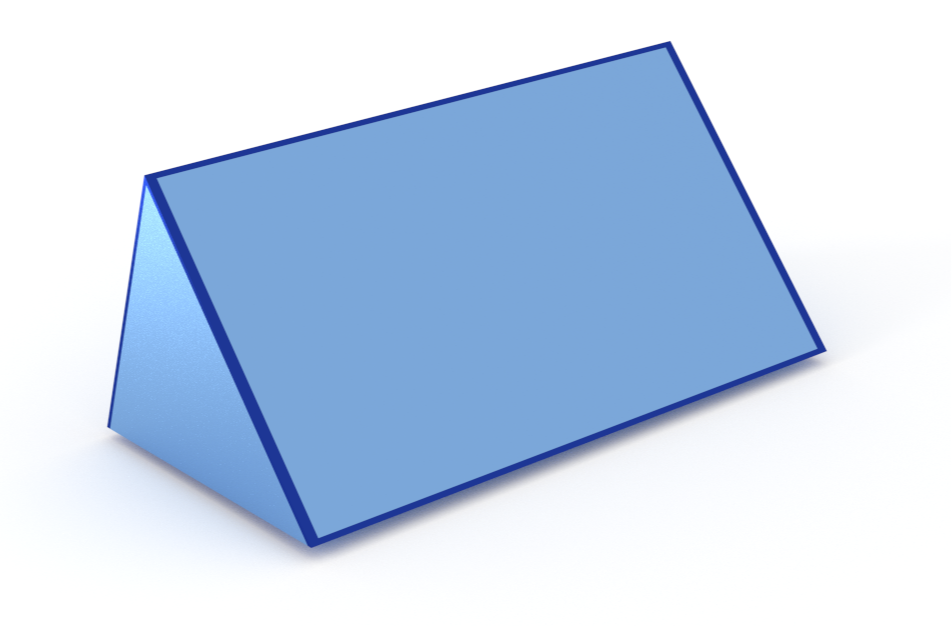
\includegraphics[width=1in]{Figures/Ripple23d}  \\
\hline 
\end{tabulary}
\end{table}

In \BornAgain\ the form factor is defined as
\begin{equation}
F(\mathbf{q})=\int_V \exp (i\mathbf{q}.\mathbf{r}) d^3 \mathbf{r},
\label{ffformulaBA}
\end{equation}
where $V$ is the volume of the particle's shape,
$\mathbf{q}=\mathbf{k}_i - \mathbf{k}_f$ is the scattering vector with
$\mathbf{k}_f$ and $\mathbf{k}_i$ the scattered and incident wave
vector, respectively.\\

The particle's shape is parametrized in a cartesian frame, with its
$z$-axis pointing upwards and its origin at the center of the bottom
of the particle: $\mathbf{r}=(x,y,z)$. In the followings, a schematic view will depict this layout for each
form factor.\\


All form factors have been implemented with complex scattering vectors
in order to take any material absorption into account.\\


The particles can be rotated in a different direction by using one of
the following transformations: \Code{CreateRotateX($\theta$),
  CreateRotateY($\theta$), CreateRotateZ($\theta$)}, where capital X, Y, Z mark rotations
around the associated axis and $\theta$ is the
angle of rotation from this axis. For example, in order to rotate a pyramid by $45^{\circ}$ around
$z$-axis, the user could use the following \Code{Python}\ script:\\

\begin{lstlisting}[language=python, style=eclipseboxed,numbers=none,nolol]
    pyramid_ff = FormFactorPyramid(10*nanometer, 5*nanometer, deg2rad(54.73 ) )
    pyramid = Particle(m_particle, pyramid_ff)
    angle_around_z = 45.*degree
    transform = Transform3D.createRotateZ(angle_around_z)
    particle_layout = ParticleLayout()
    particle_layout.addParticle(pyramid, transform) 
\end{lstlisting}

\newpage
%%%%%%%%%%%%%%%%%%%%%%%%%%%%%%%%%%%%
%\section{Parallelepiped} \SecLabel{Parallelepiped}  

%\subsection{Real-space geometry}
%This shape is a square cuboid (see fig.~\ref{fig:parallelepiped}).

%\begin{figure}[ht]
%\hfill
%\subfigure[Side view]{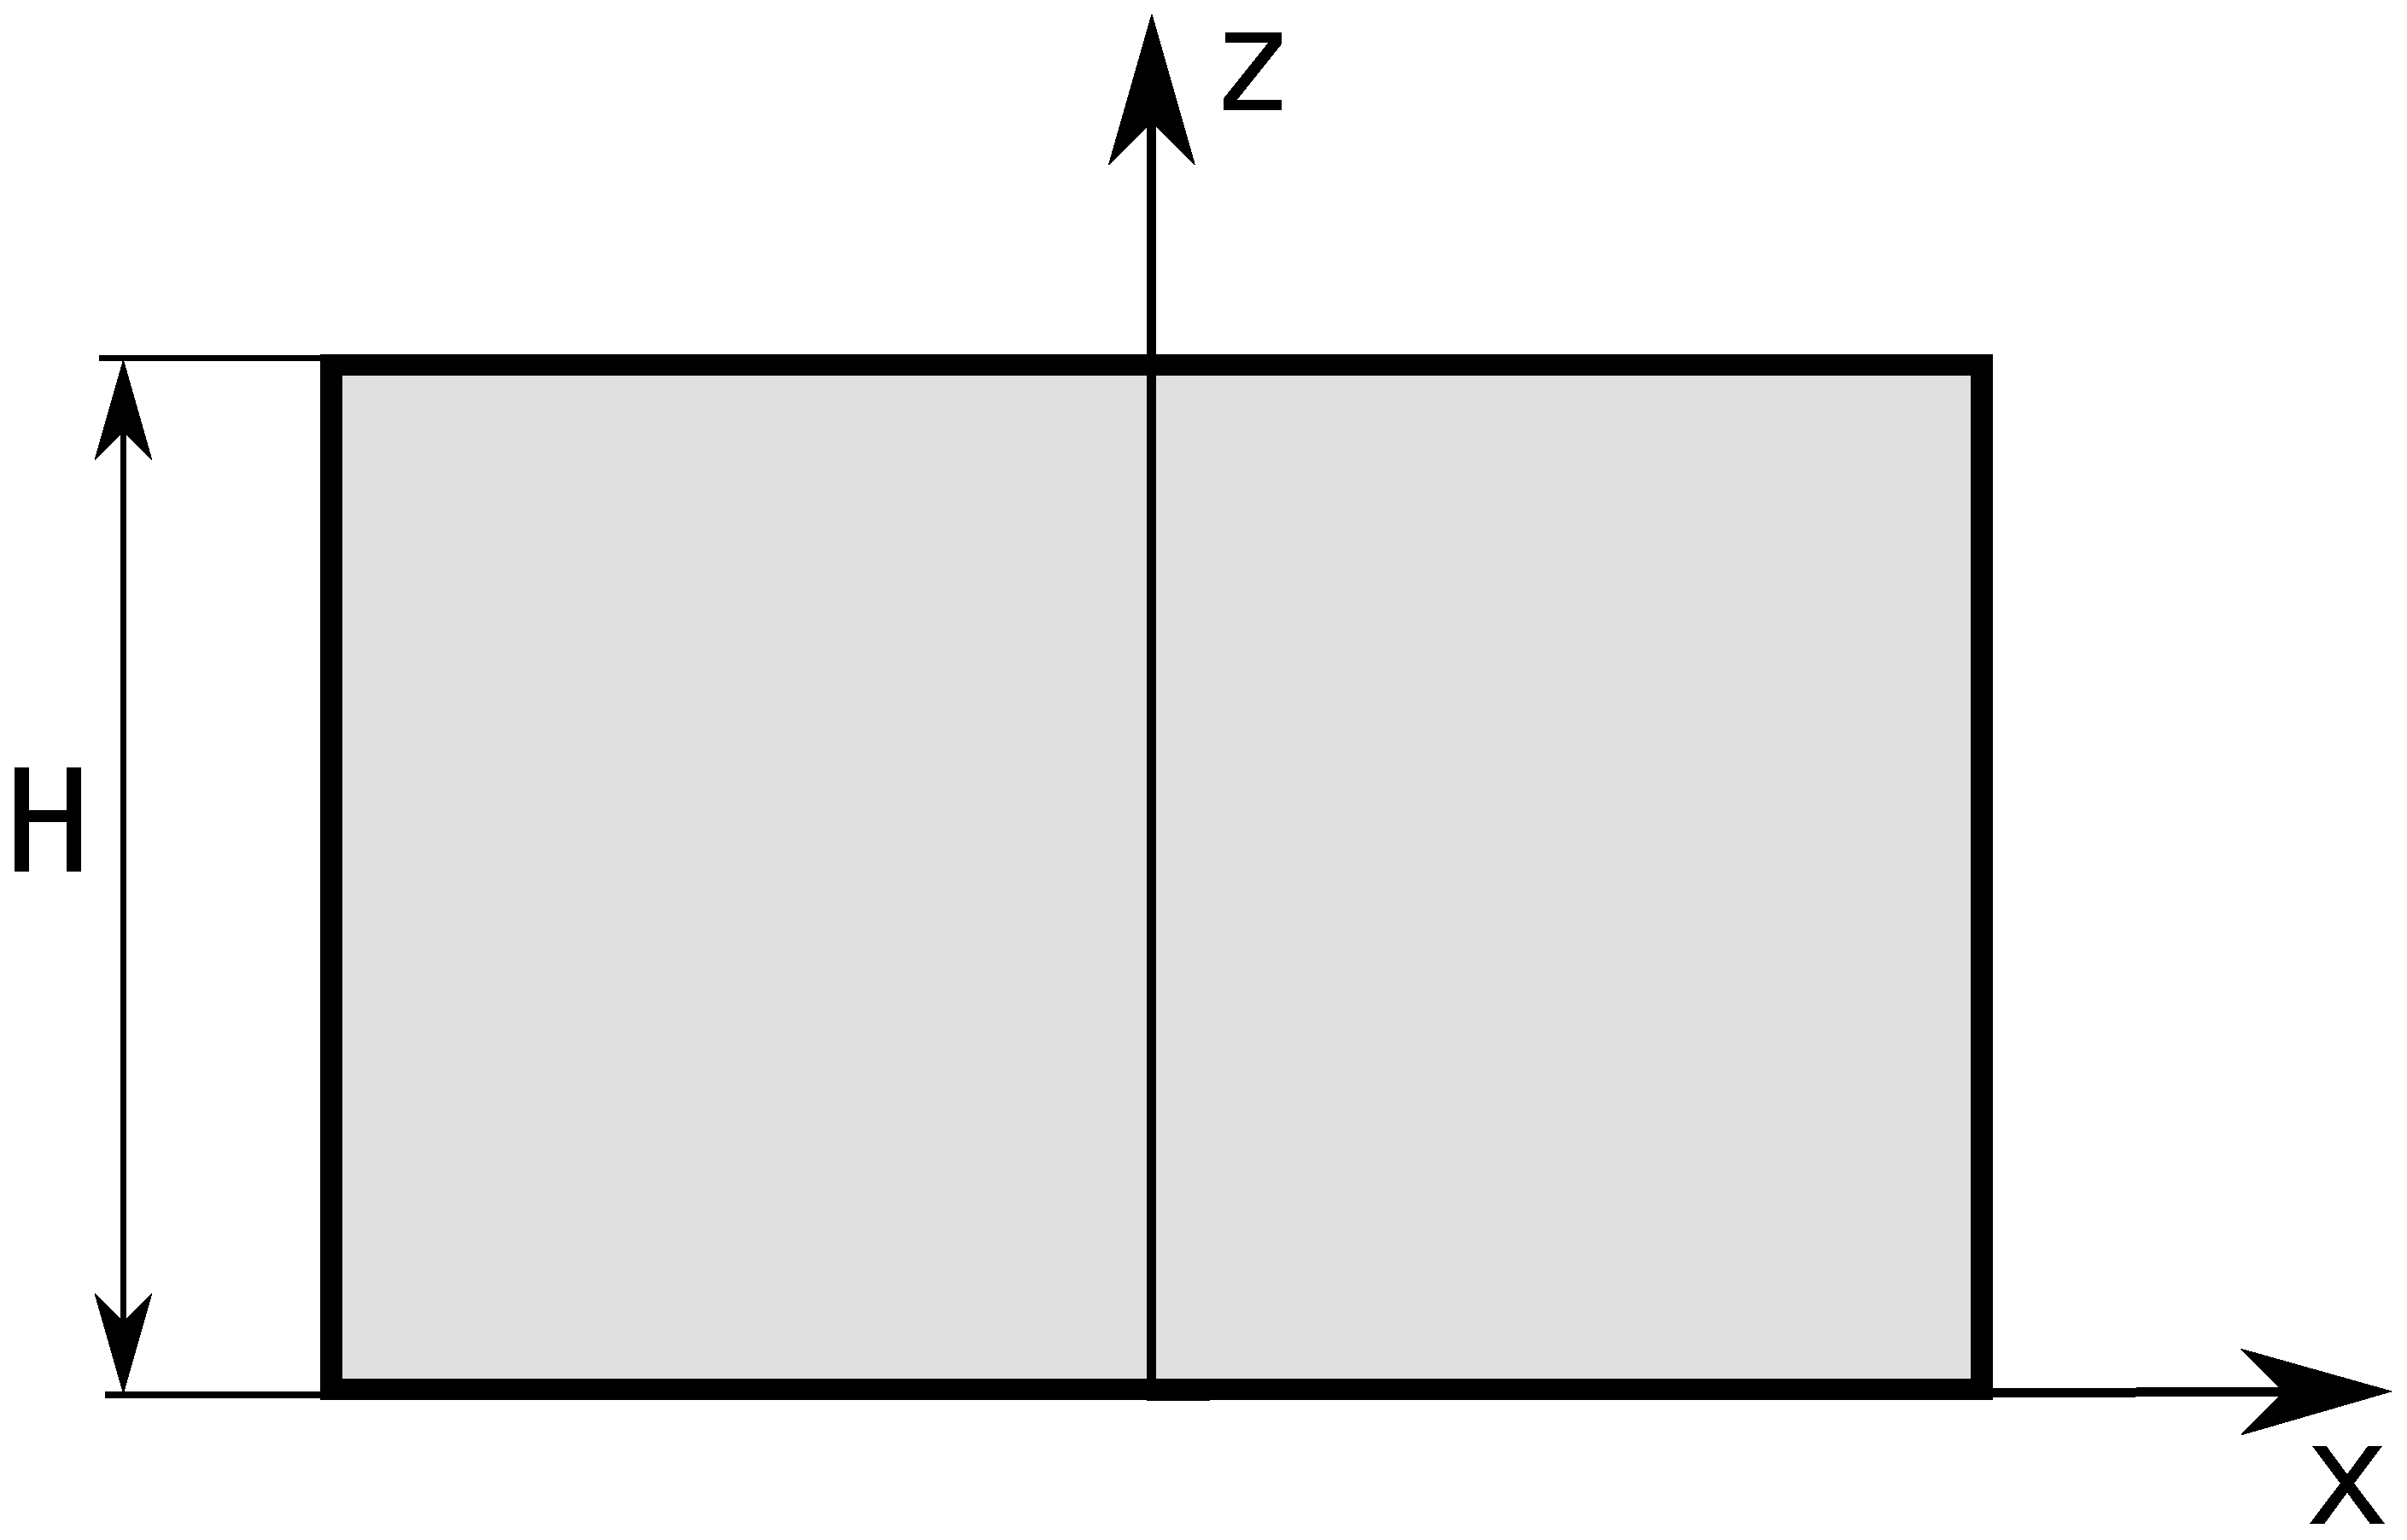
\includegraphics[width=5cm]{Figures/Parallelepiped2dxz}}
%\hfill
%\subfigure[Top view]{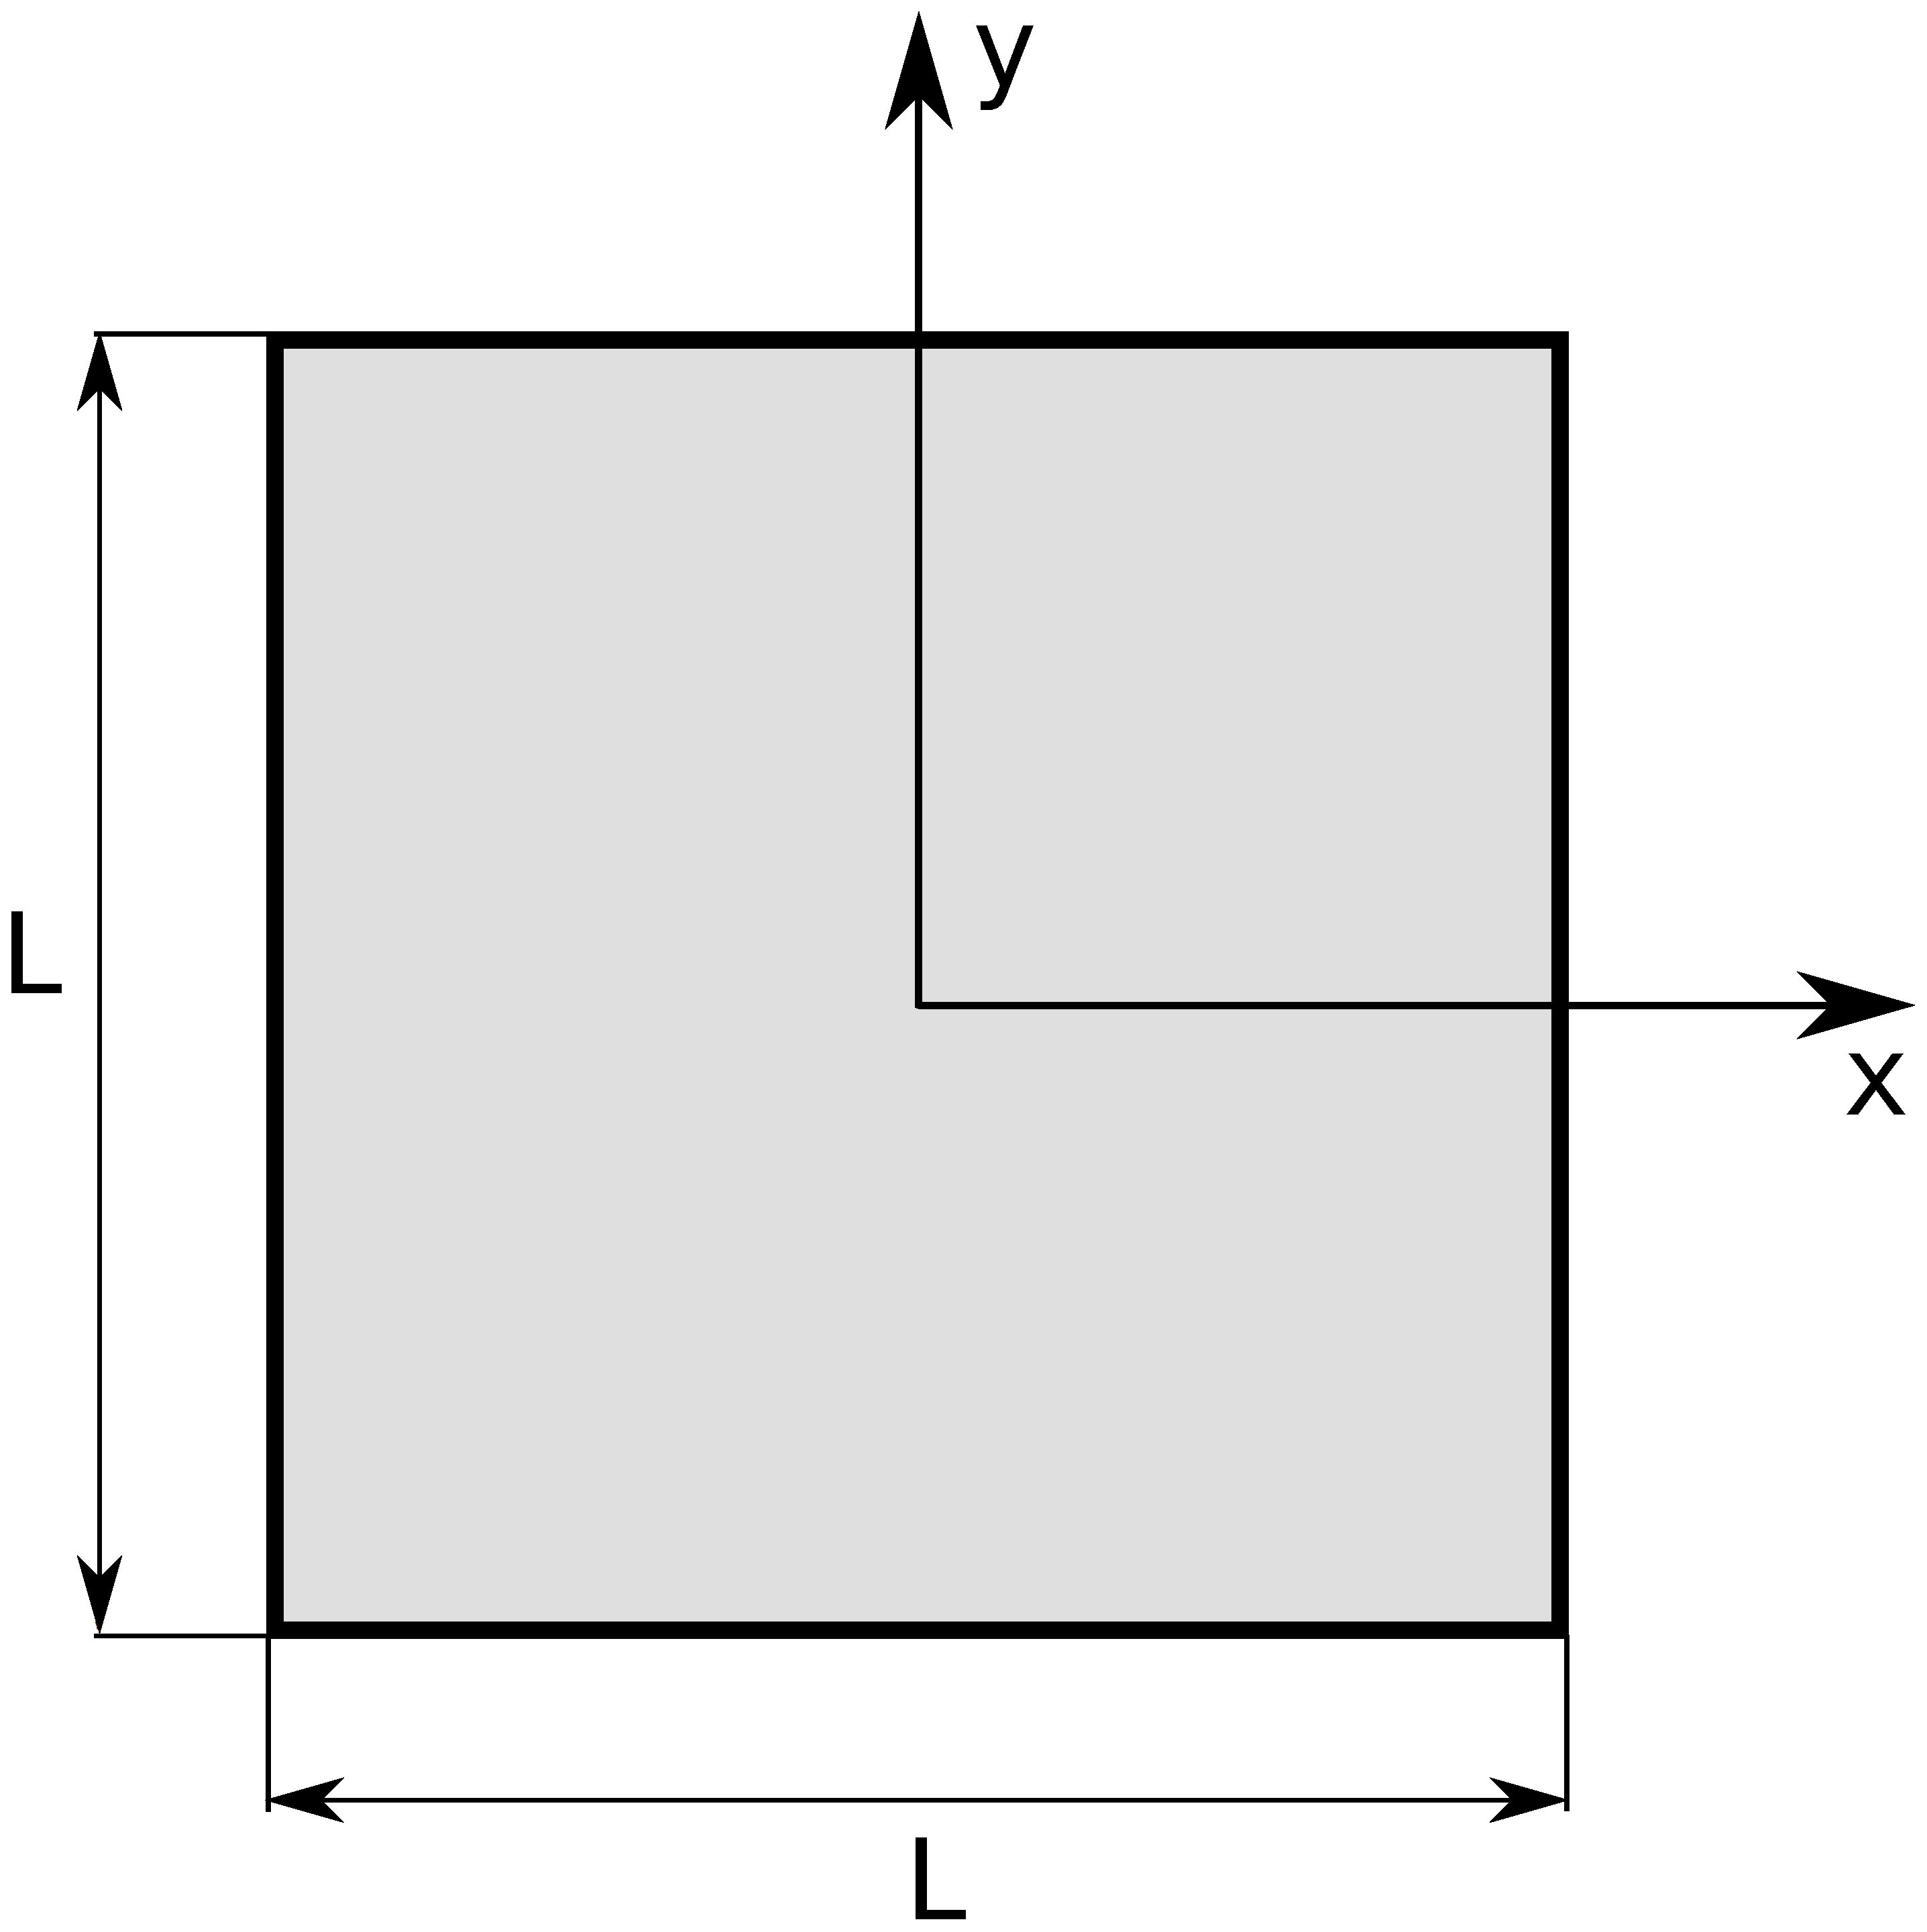
\includegraphics[width=5cm]{Figures/Parallelepiped2dxy}}
%\hfill
%\caption{Sketch of a Parallelepiped.}
%\label{fig:parallelepiped}
%\end{figure}

%\FloatBarrier

%\paragraph{Parameters:}
%\begin{itemize}
%\item length of one side of the square base $L$,
%\item height $H$.
%\end{itemize}

%\paragraph{Properties:}
%\begin{itemize}
%\item volume $V= L^2 H$,
%\item particle surface seen from above $S =L^2$.
%\end{itemize}

%\subsection{Expression of the form factor}
%\begin{equation*}
%F_{\rm{Parallelepiped}}(\mathbf{q},L, H) = L^2 H\exp\left(i q_z \frac{H}{2}\right) \sinc\left(q_x\frac{L}{2}\right)
%\sinc\left(q_y\frac{L}{2}\right)\sinc\left(q_z \frac{H}{2}\right),
%\end{equation*}
%where $\sinc(x)=\sin(x)/x$ is the cardinal sine.

%\paragraph{Syntax:} \Code{FormFactorParallelepiped(length, height)}

%\newpage

%\subsection{Examples}

%Figure~\ref{fig:FFparallelEx} shows the normalized intensity
%$|F|^2/V^2$, computed with $L=7$~nm and \mbox{$H=15$~nm.}

%\begin{figure}[h]
%\begin{center}
%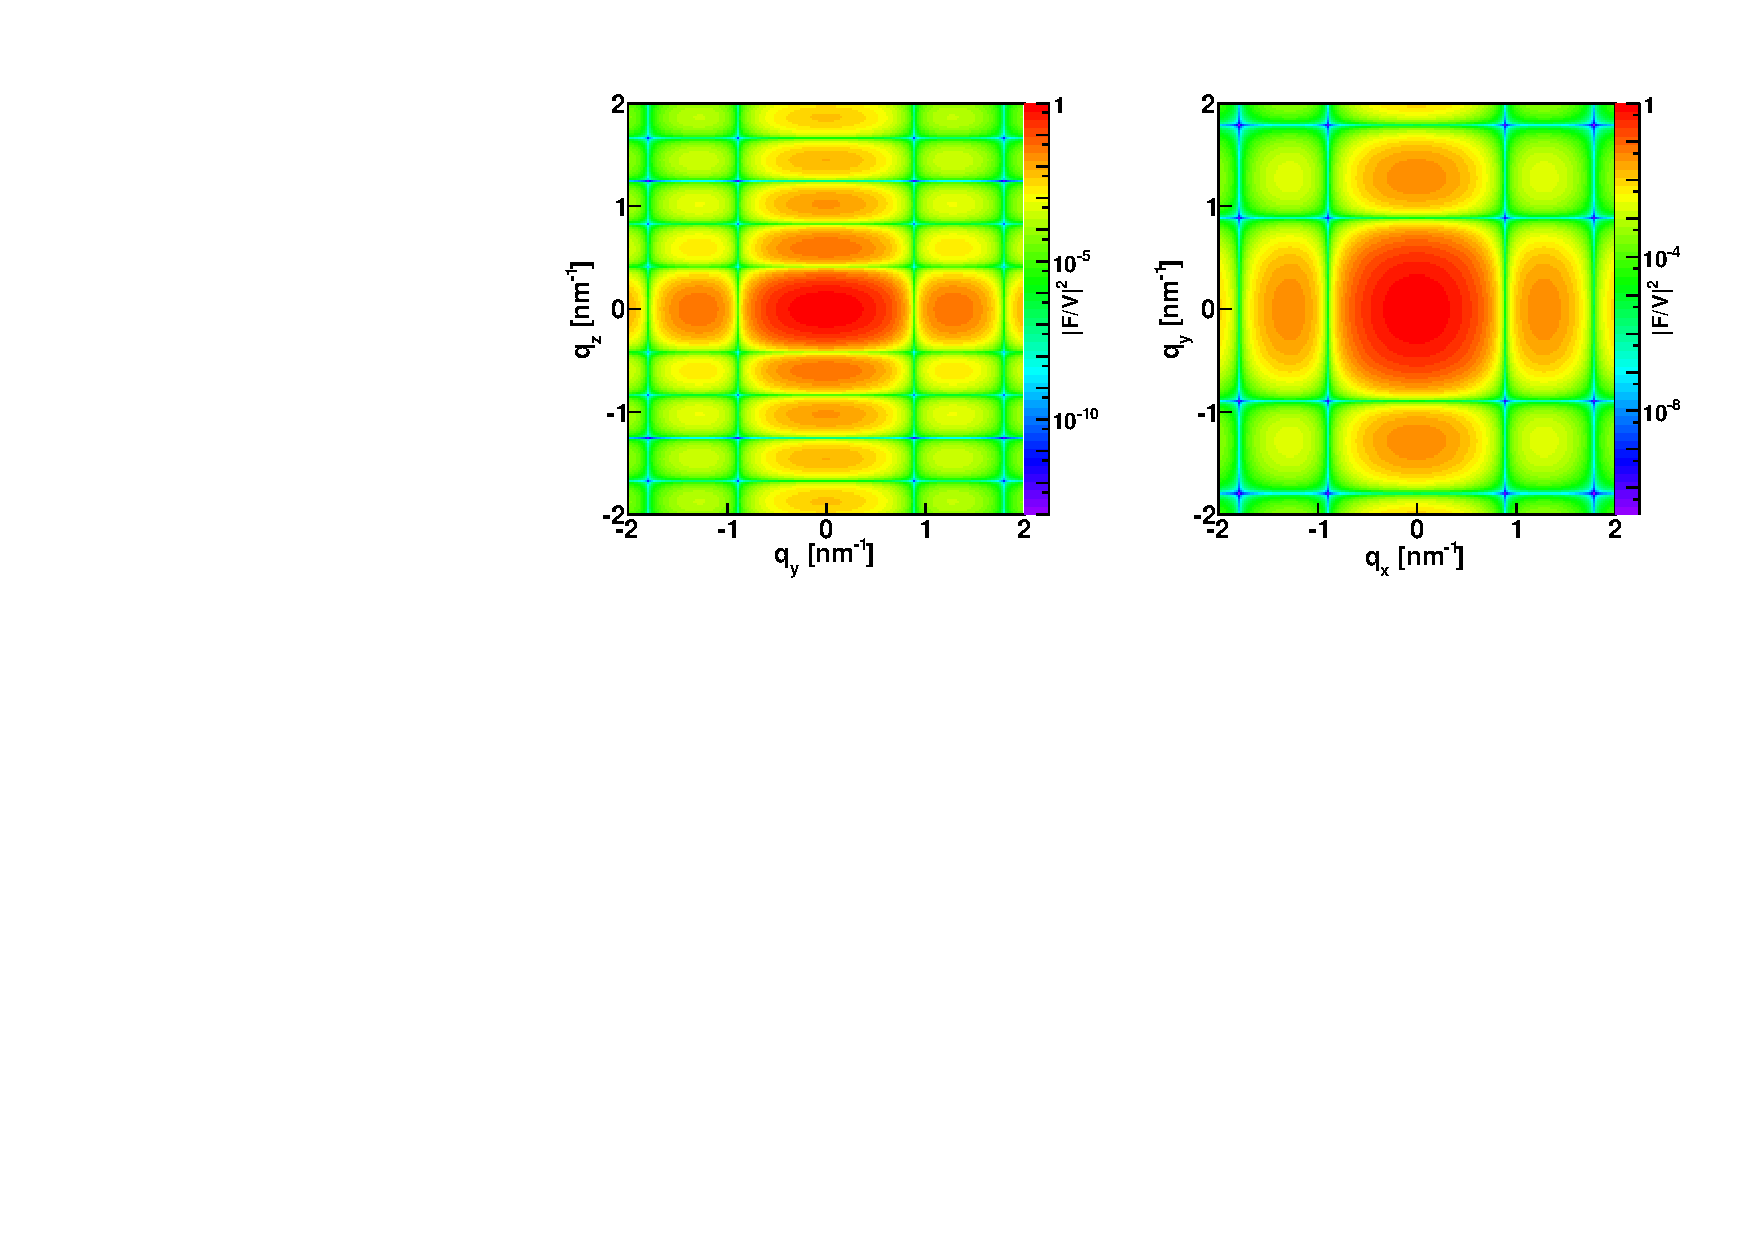
\includegraphics[width=\textwidth]{Figures/figffparallel}
%\end{center}
%\caption{Normalized intensity for the form factor of a Parallelepiped
%  $|F|^2/V^2$, plotted against ($q_z$, $q_y$) and  ($q_x$, $q_y$) and computed with $L=7$~nm and $H=15$~nm.}
%\label{fig:FFparallelEx}
%\end{figure}

%\FloatBarrier

%\newpage{\cleardoublepage}
%%%%%%%%%%%%%%%%%%%%%%%%%%%%%%%%%%%%
\section{Box} \SecLabel{Box} 

\subsection{Real-space geometry}
This shape is a rectangular cuboid as
shown in fig.~\ref{fig:box}. 


\begin{figure}[ht]
\hfill
\subfigure[Side view]{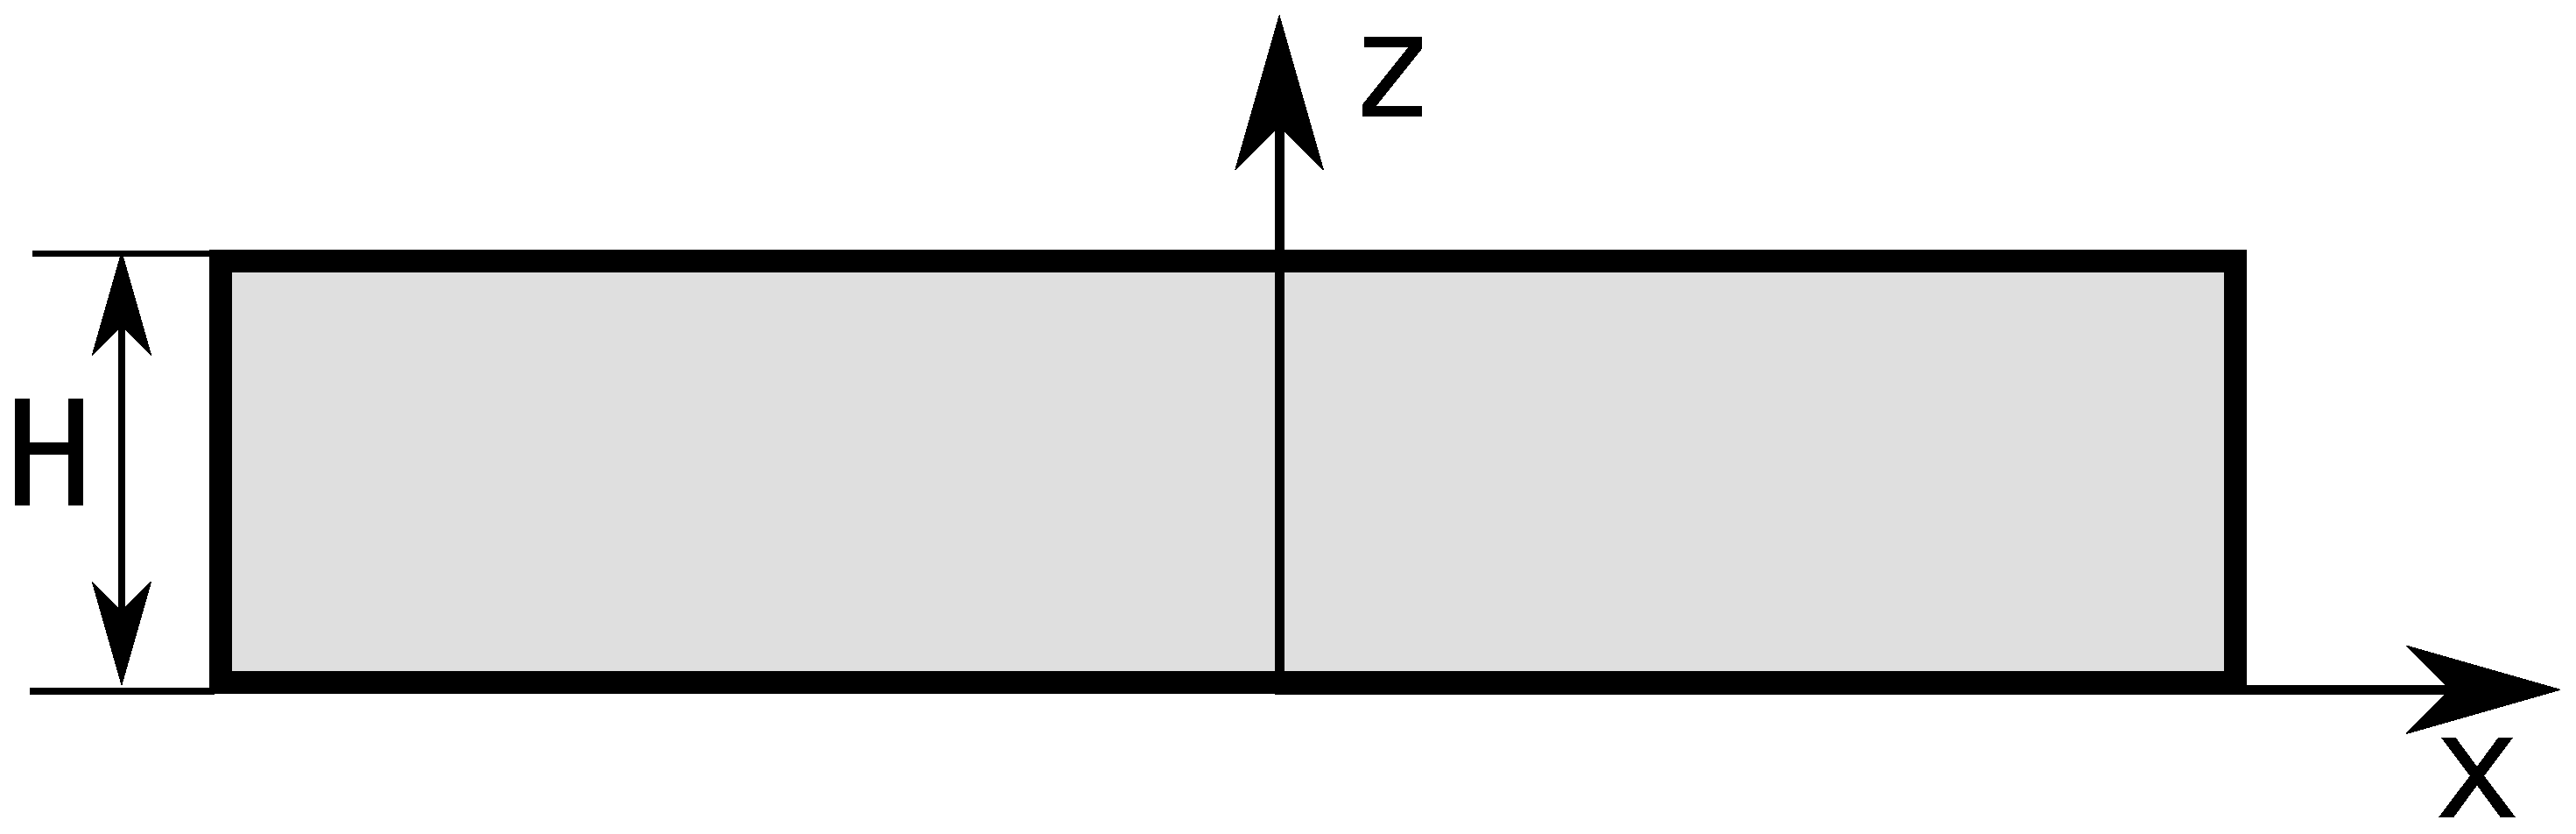
\includegraphics[width=5cm]{Figures/Box2dxz}}
\hfill
\subfigure[Top view]{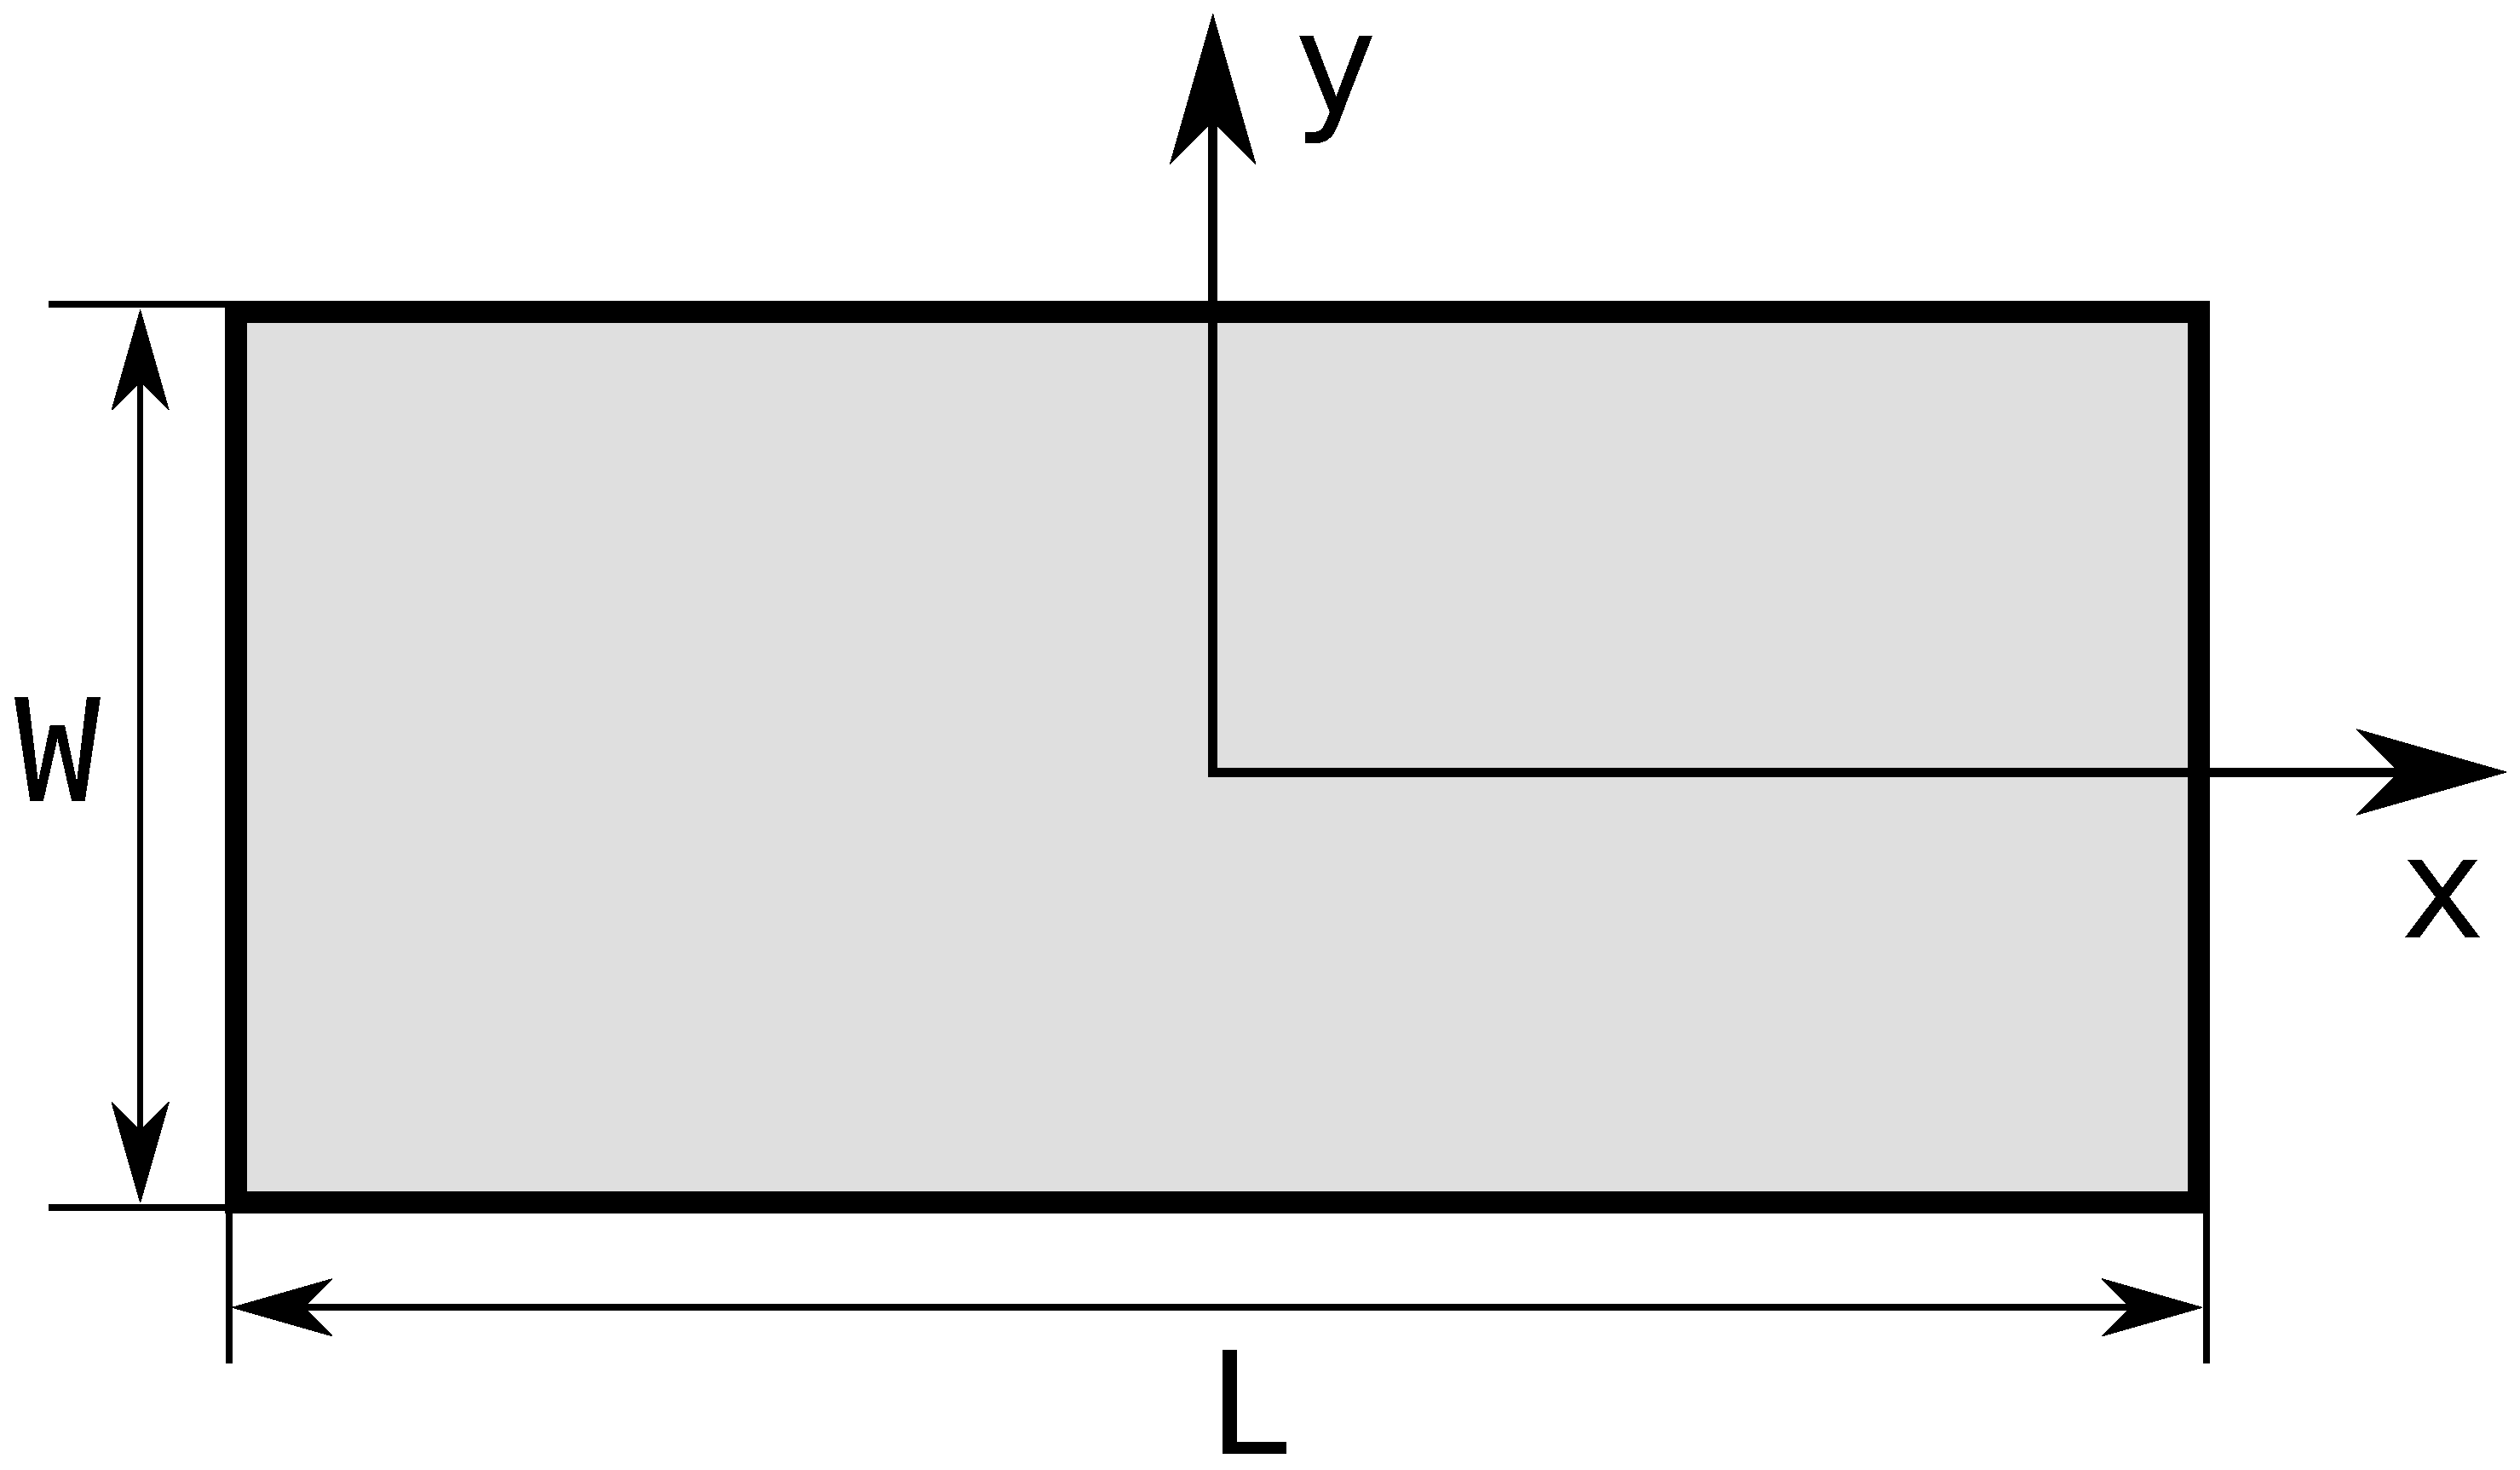
\includegraphics[width=5cm]{Figures/Box2dxy}}
\hfill
\caption{Sketch of a Box.}
\label{fig:box}
\end{figure}

\FloatBarrier


\paragraph{Parameters:}
\begin{itemize}
\item length of the base $L$,
\item width of the base $W$,
\item height  $H$.
\end{itemize}

\paragraph{Properties:}
\begin{itemize}
\item volume $V= LWH$,
\item particle surface seen from above $S = LW$.
%\item radius of gyration
\end{itemize}

\subsection{Expression of the form factor}

\begin{equation*}
F_{\rm{Box}}(\mathbf{q},L,W,H)= L W H\exp\left(i q_z \frac{H}{2}\right) \sinc\left(q_x \frac{L}{2}\right)
\sinc\left(q_y \frac{W}{2}\right) \sinc\left(q_z \frac{H}{2}\right),
\end{equation*}
    
where $\sinc(x)=\sin(x)/x$ is the cardinal sine.

\paragraph{Syntax:} \Code{FormFactorBox(length, width, height)}

\newpage

\subsection{Examples}
Figure~\ref{fig:FFBoxEx} shows the normalized intensity
$|F|^2/V^2$, computed with $L=20$~nm, $W=16$~nm, $H=13$~nm, and
$\alpha=60^{\circ}$:

\begin{figure}[h]
\begin{center}
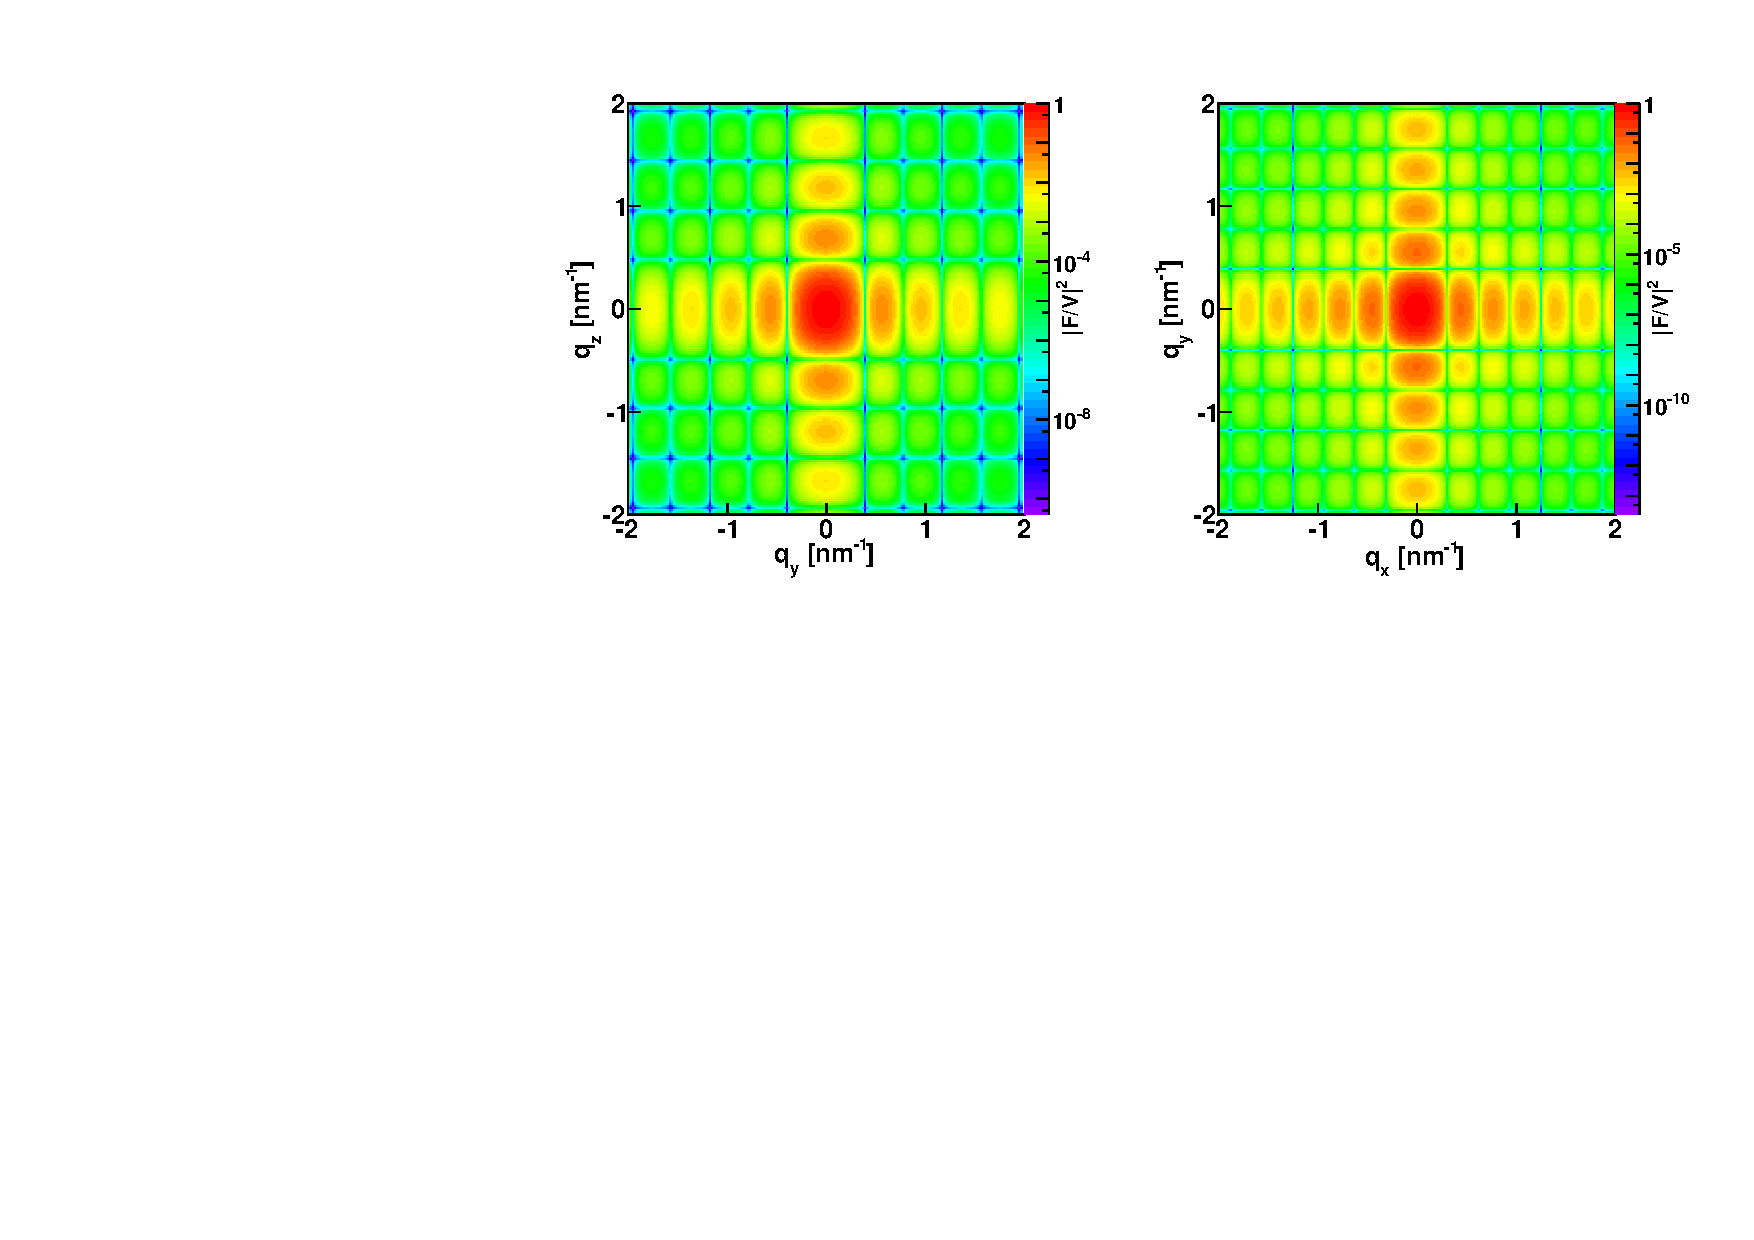
\includegraphics[width=\textwidth]{Figures/figffbox}
\end{center}
\caption{Normalized intensity for the form factor of a Box
  $|F|^2/V^2$, plotted against ($q_z$, $q_y$) and  ($q_x$, $q_y$) and computed with $L=20$~nm, $W=16$~nm, and $H=13$~nm.}
\label{fig:FFBoxEx}
\end{figure}

\FloatBarrier

%\subsection{References}
%\BornAgain\ uses a different convention for the parameters in comparison with \Code{IsGISAXS}, where the half length
%values are used (see fig.~\ref{box}).

\newpage{\cleardoublepage}
%%%%%%%%%%%%%%%%%%%%%%%%%%%%%%%%%%%%
\section{Prism3} \SecLabel{Prism3}
 
\subsection{Real-space geometry}
This shape is a triangular prism, whose base is an equilateral
triangle as shown in fig.~\ref{fig:prism3}.

\begin{figure}[ht]
\hfill
\subfigure[Side view]{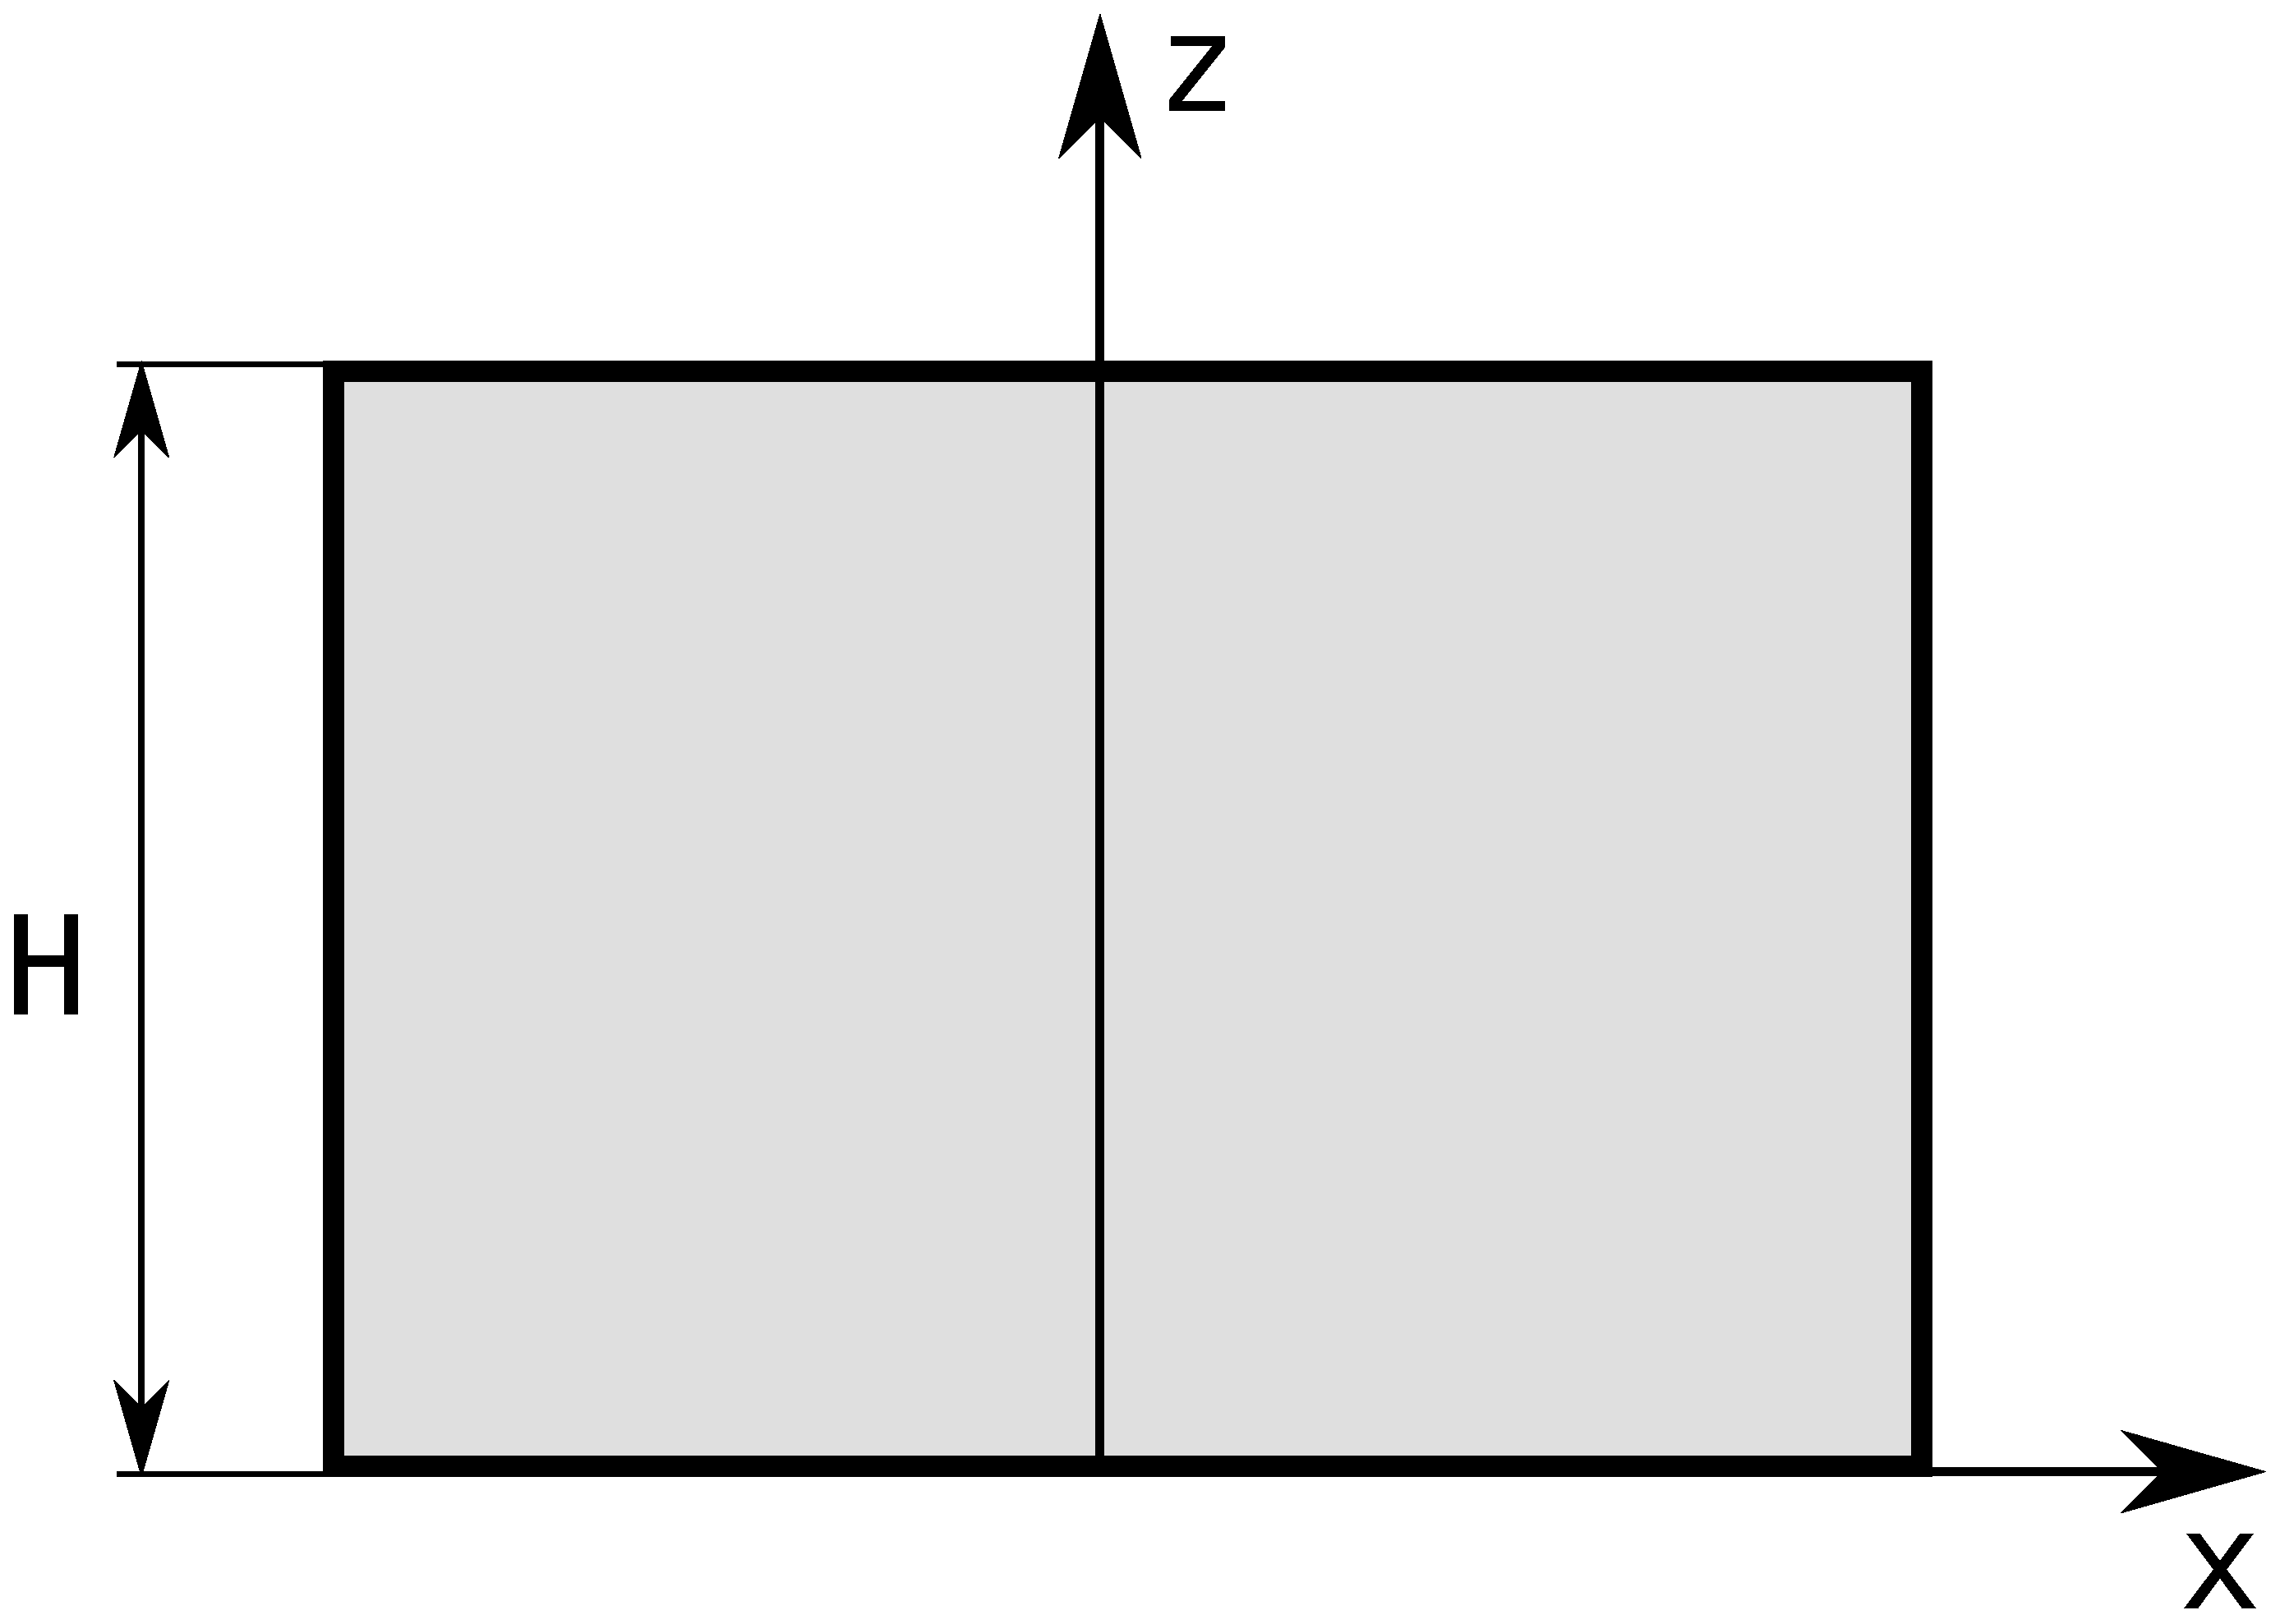
\includegraphics[width=5cm]{Figures/Prism32dxz}}
\hfill
\subfigure[Top view]{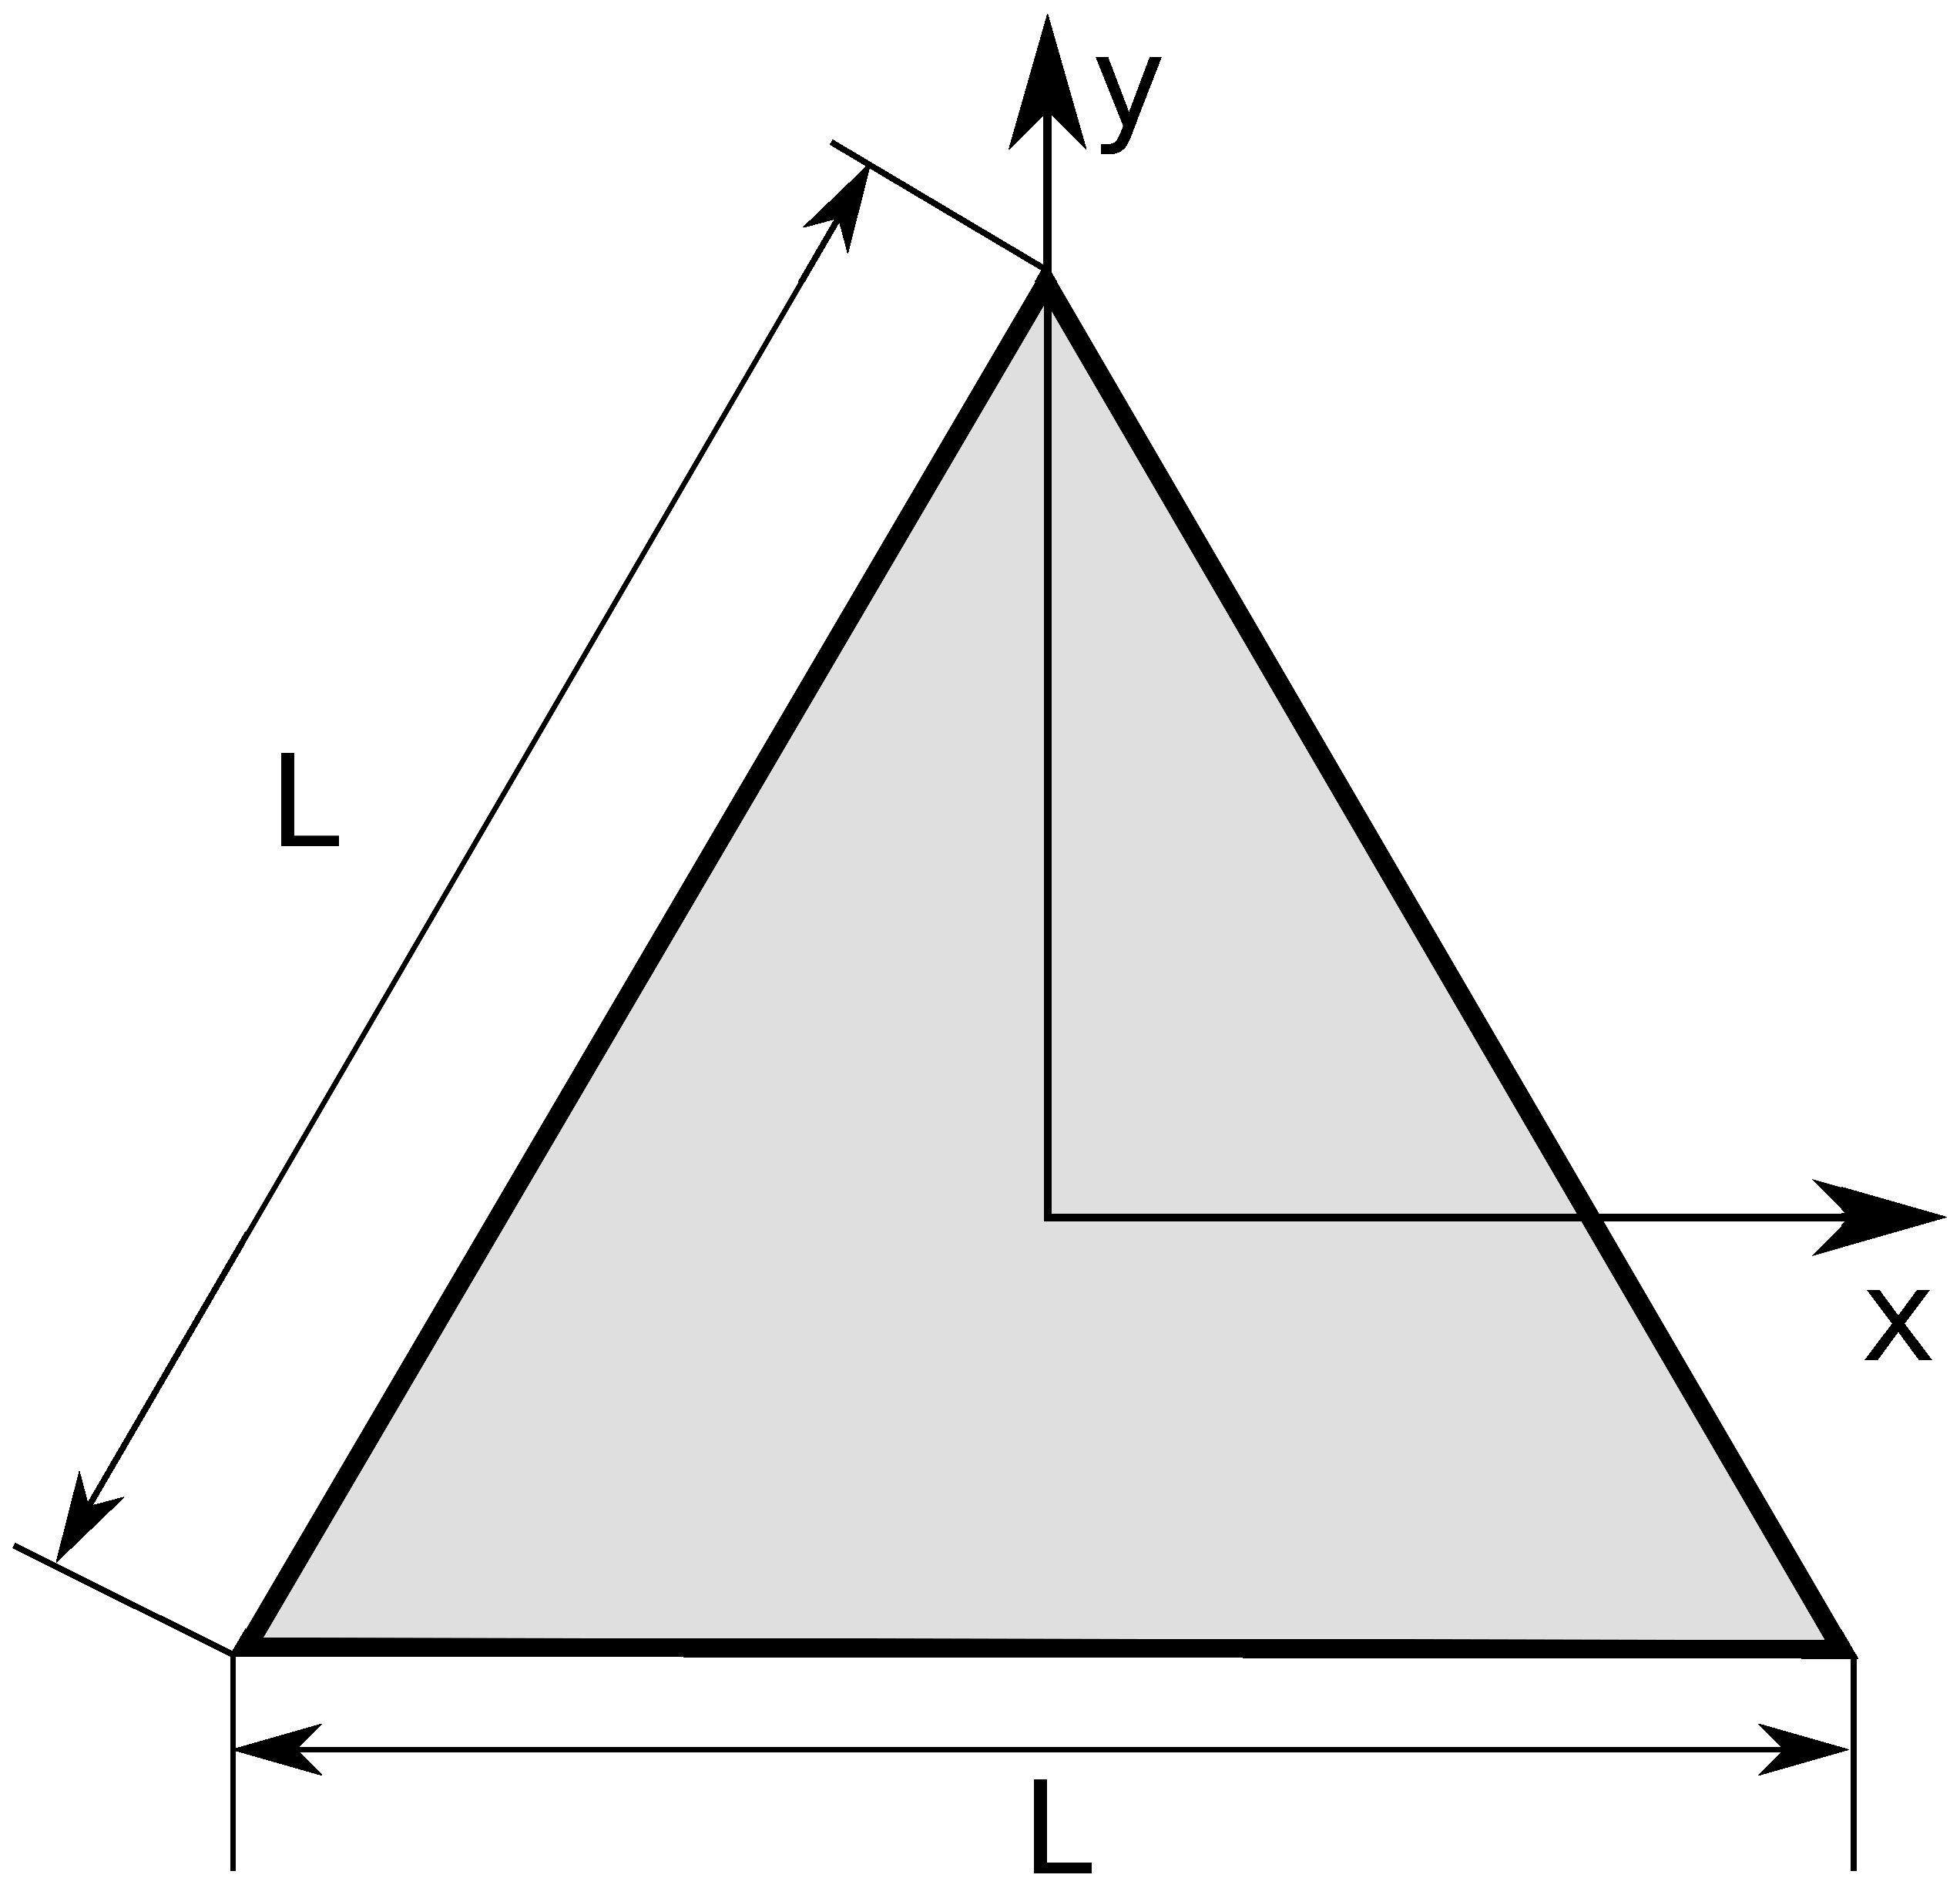
\includegraphics[width=5cm]{Figures/Prism32dxy}}
\hfill
\caption{Sketch of a Prism3.}
\label{fig:prism3}
\end{figure}

\FloatBarrier

\paragraph{Parameters:}
\begin{itemize}
\item length $L$ of one side of the base, 
\item height $H$.
\end{itemize}

\paragraph{Properties:}
\begin{itemize}
\item volume $V= \dfrac{\sqrt{3}}{4} H L^2$,
\item particle surface seen from above $S =\dfrac{\sqrt{3}}{4}L^2$.
%\item radius of gyration.
\end{itemize}

\subsection{Expression of the form factor}
\begin{align*}
F_{\rm{Prism3}}(\mathbf{q},L, H) &= \frac{2 \sqrt{3}}{q_x^2-3q_y^2}  \exp\left(-i q_y\frac{L}{2\sqrt{3}}\right)\left[\exp\left(i \sqrt{3} q_y \frac{L}{2} \right)-\cos\left(q_x \frac{L}{2}\right)-i \sqrt{3} q_y \frac{L}{2} \sinc\left(q_x \frac{L}{2}\right) \right] \\
  &
\times  H \sinc\left(q_z \frac{H}{2} \right) \exp\left(i q_z \frac{H}{2}\right),
\end{align*}
where $\sinc(x)=\sin(x)/x$ is the cardinal sine.


\paragraph{Syntax:}  \Code{FormFactorPrism3(length, height)}

\subsection{Examples}
Figure~\ref{fig:FFprism3Ex} shows the normalized intensity
$|F|^2/V^2$, computed with $L=10$~nm and \mbox{$H=13$~nm.}
\begin{figure}[h]
\begin{center}
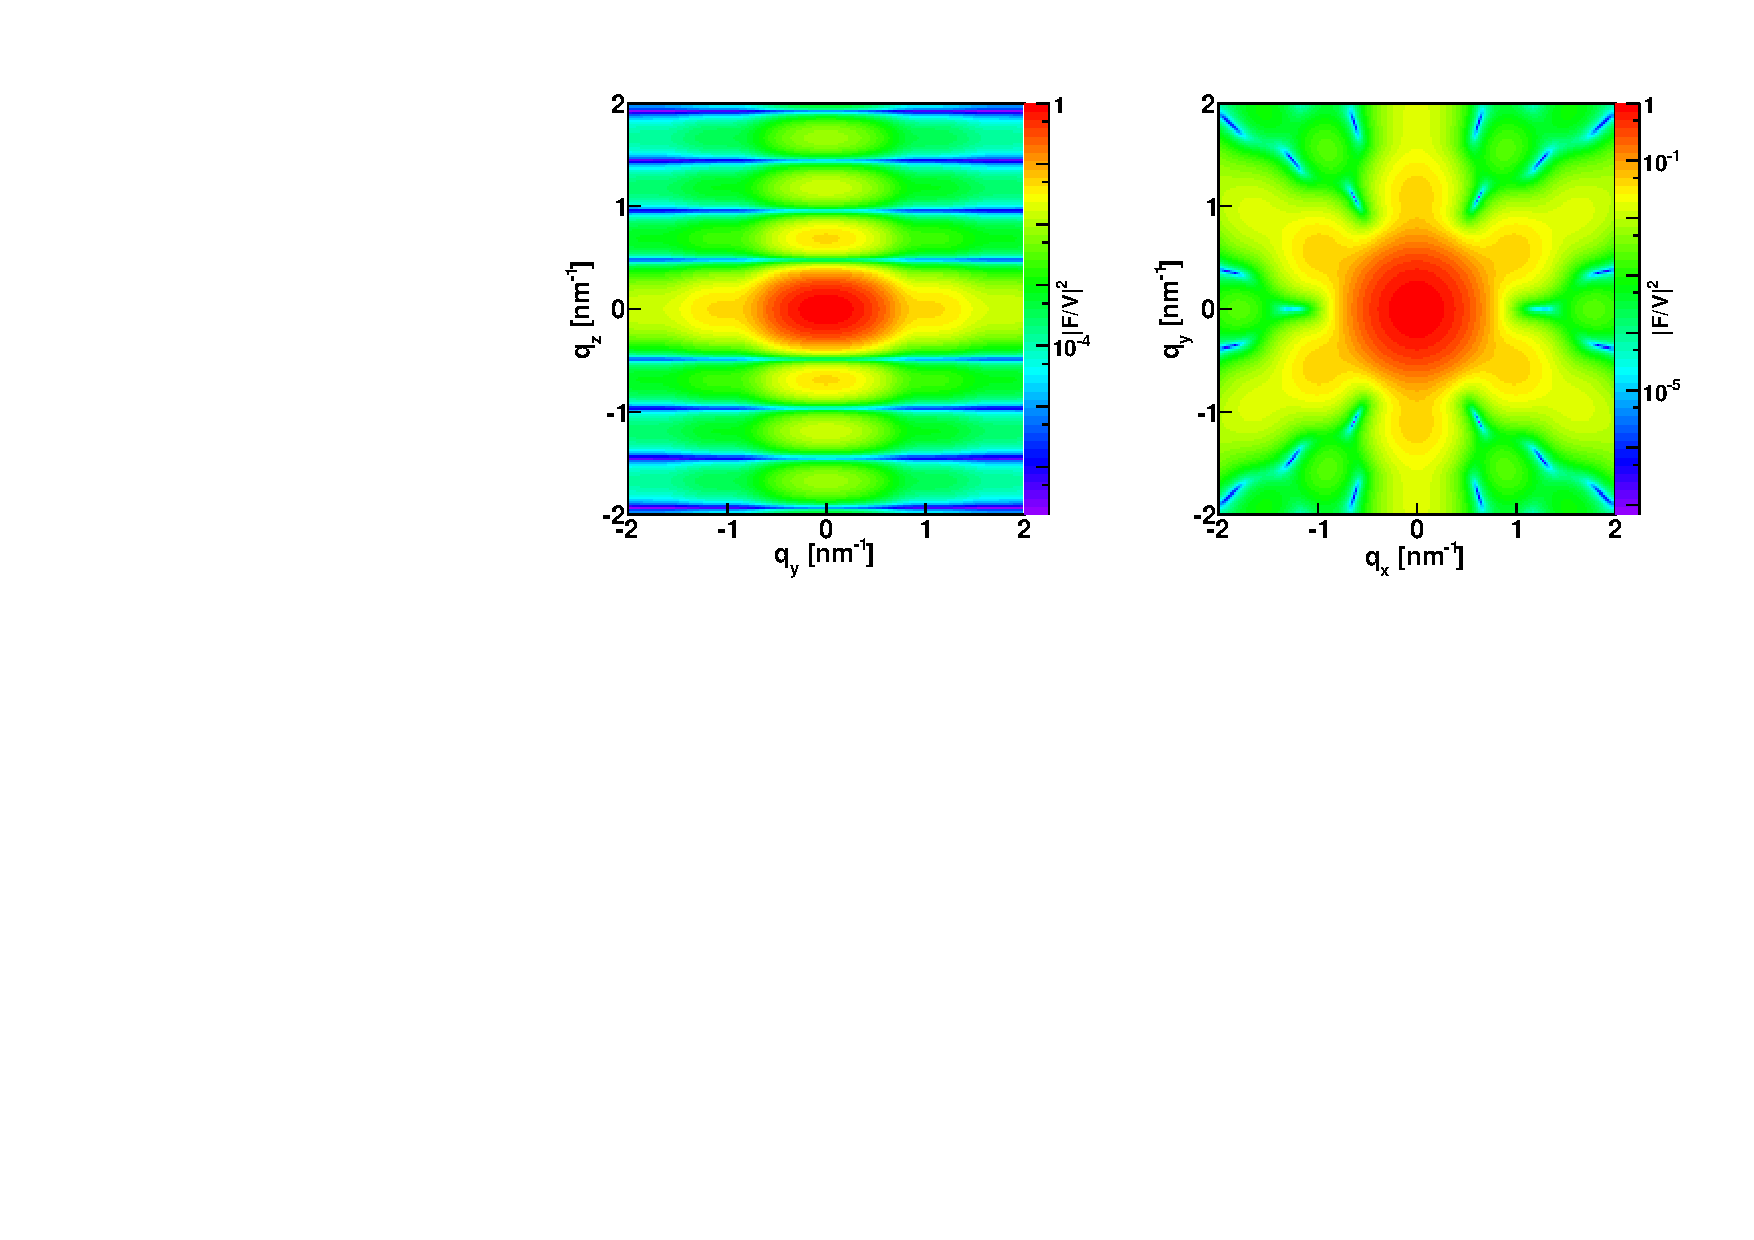
\includegraphics[width=\textwidth]{Figures/figffprism3}
\end{center}
\caption{Normalized intensity for the form factor of a Prism3
  $|F|^2/V^2$, plotted against ($q_z$, $q_y$) and  ($q_x$, $q_y$) and
  computed with $L=10$~nm and $H=13$~nm.}
\label{fig:FFprism3Ex}
\end{figure}

%\subsection{References}
%In the $x,y$ plane , we use the full side length of the triangular
%base instead of  half as implemented in \Code{IsGISAXS}: $L= 2
%R_{\rm{\Code{IsGISAXS}}}$.

\newpage{\cleardoublepage}
%%%%%%%%%%%%%%%%%%%%%%%%%%%%%%%%%%%%
\section{Tetrahedron}  \SecLabel{Tetrahedron} 
 
\subsection{Real-space geometry}
This shape is a truncated tetrahedron as shown in fig.~\ref{fig:tetrahedron}.

\begin{figure}[ht]
\hfill
\subfigure[Side view]{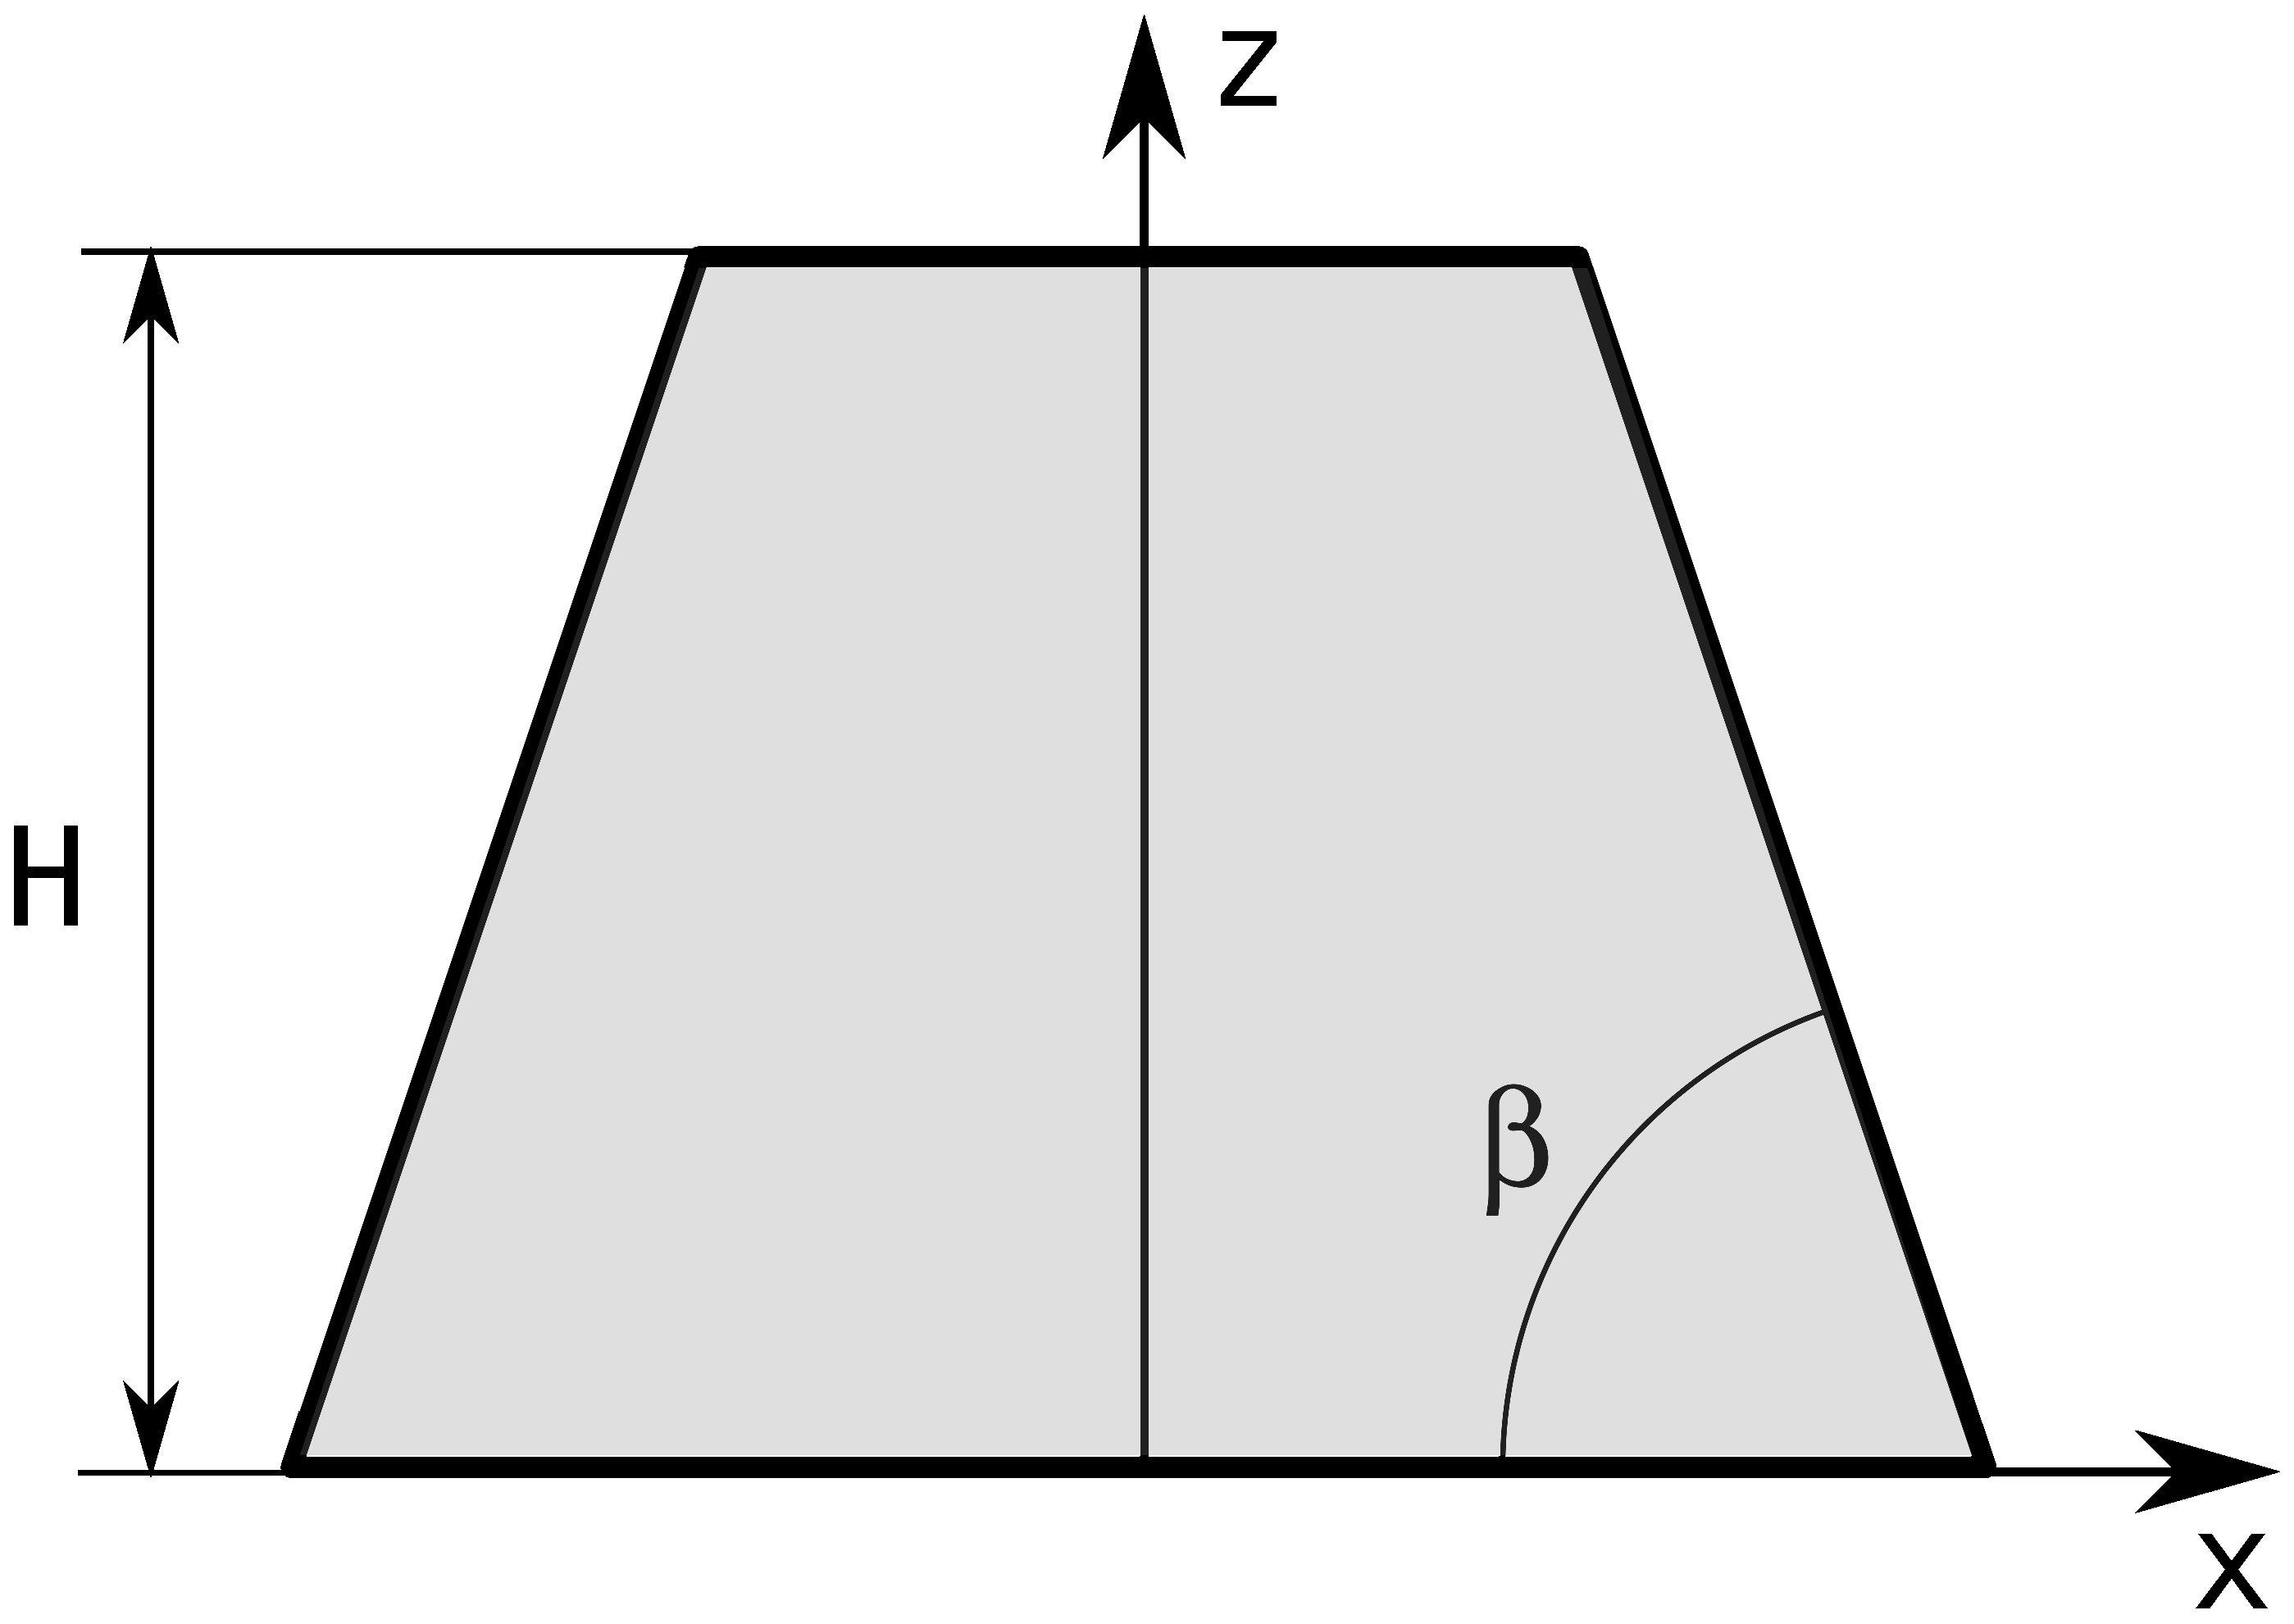
\includegraphics[width=5cm]{Figures/Tetrahedron2dxz}}
\hfill
\subfigure[Top view]{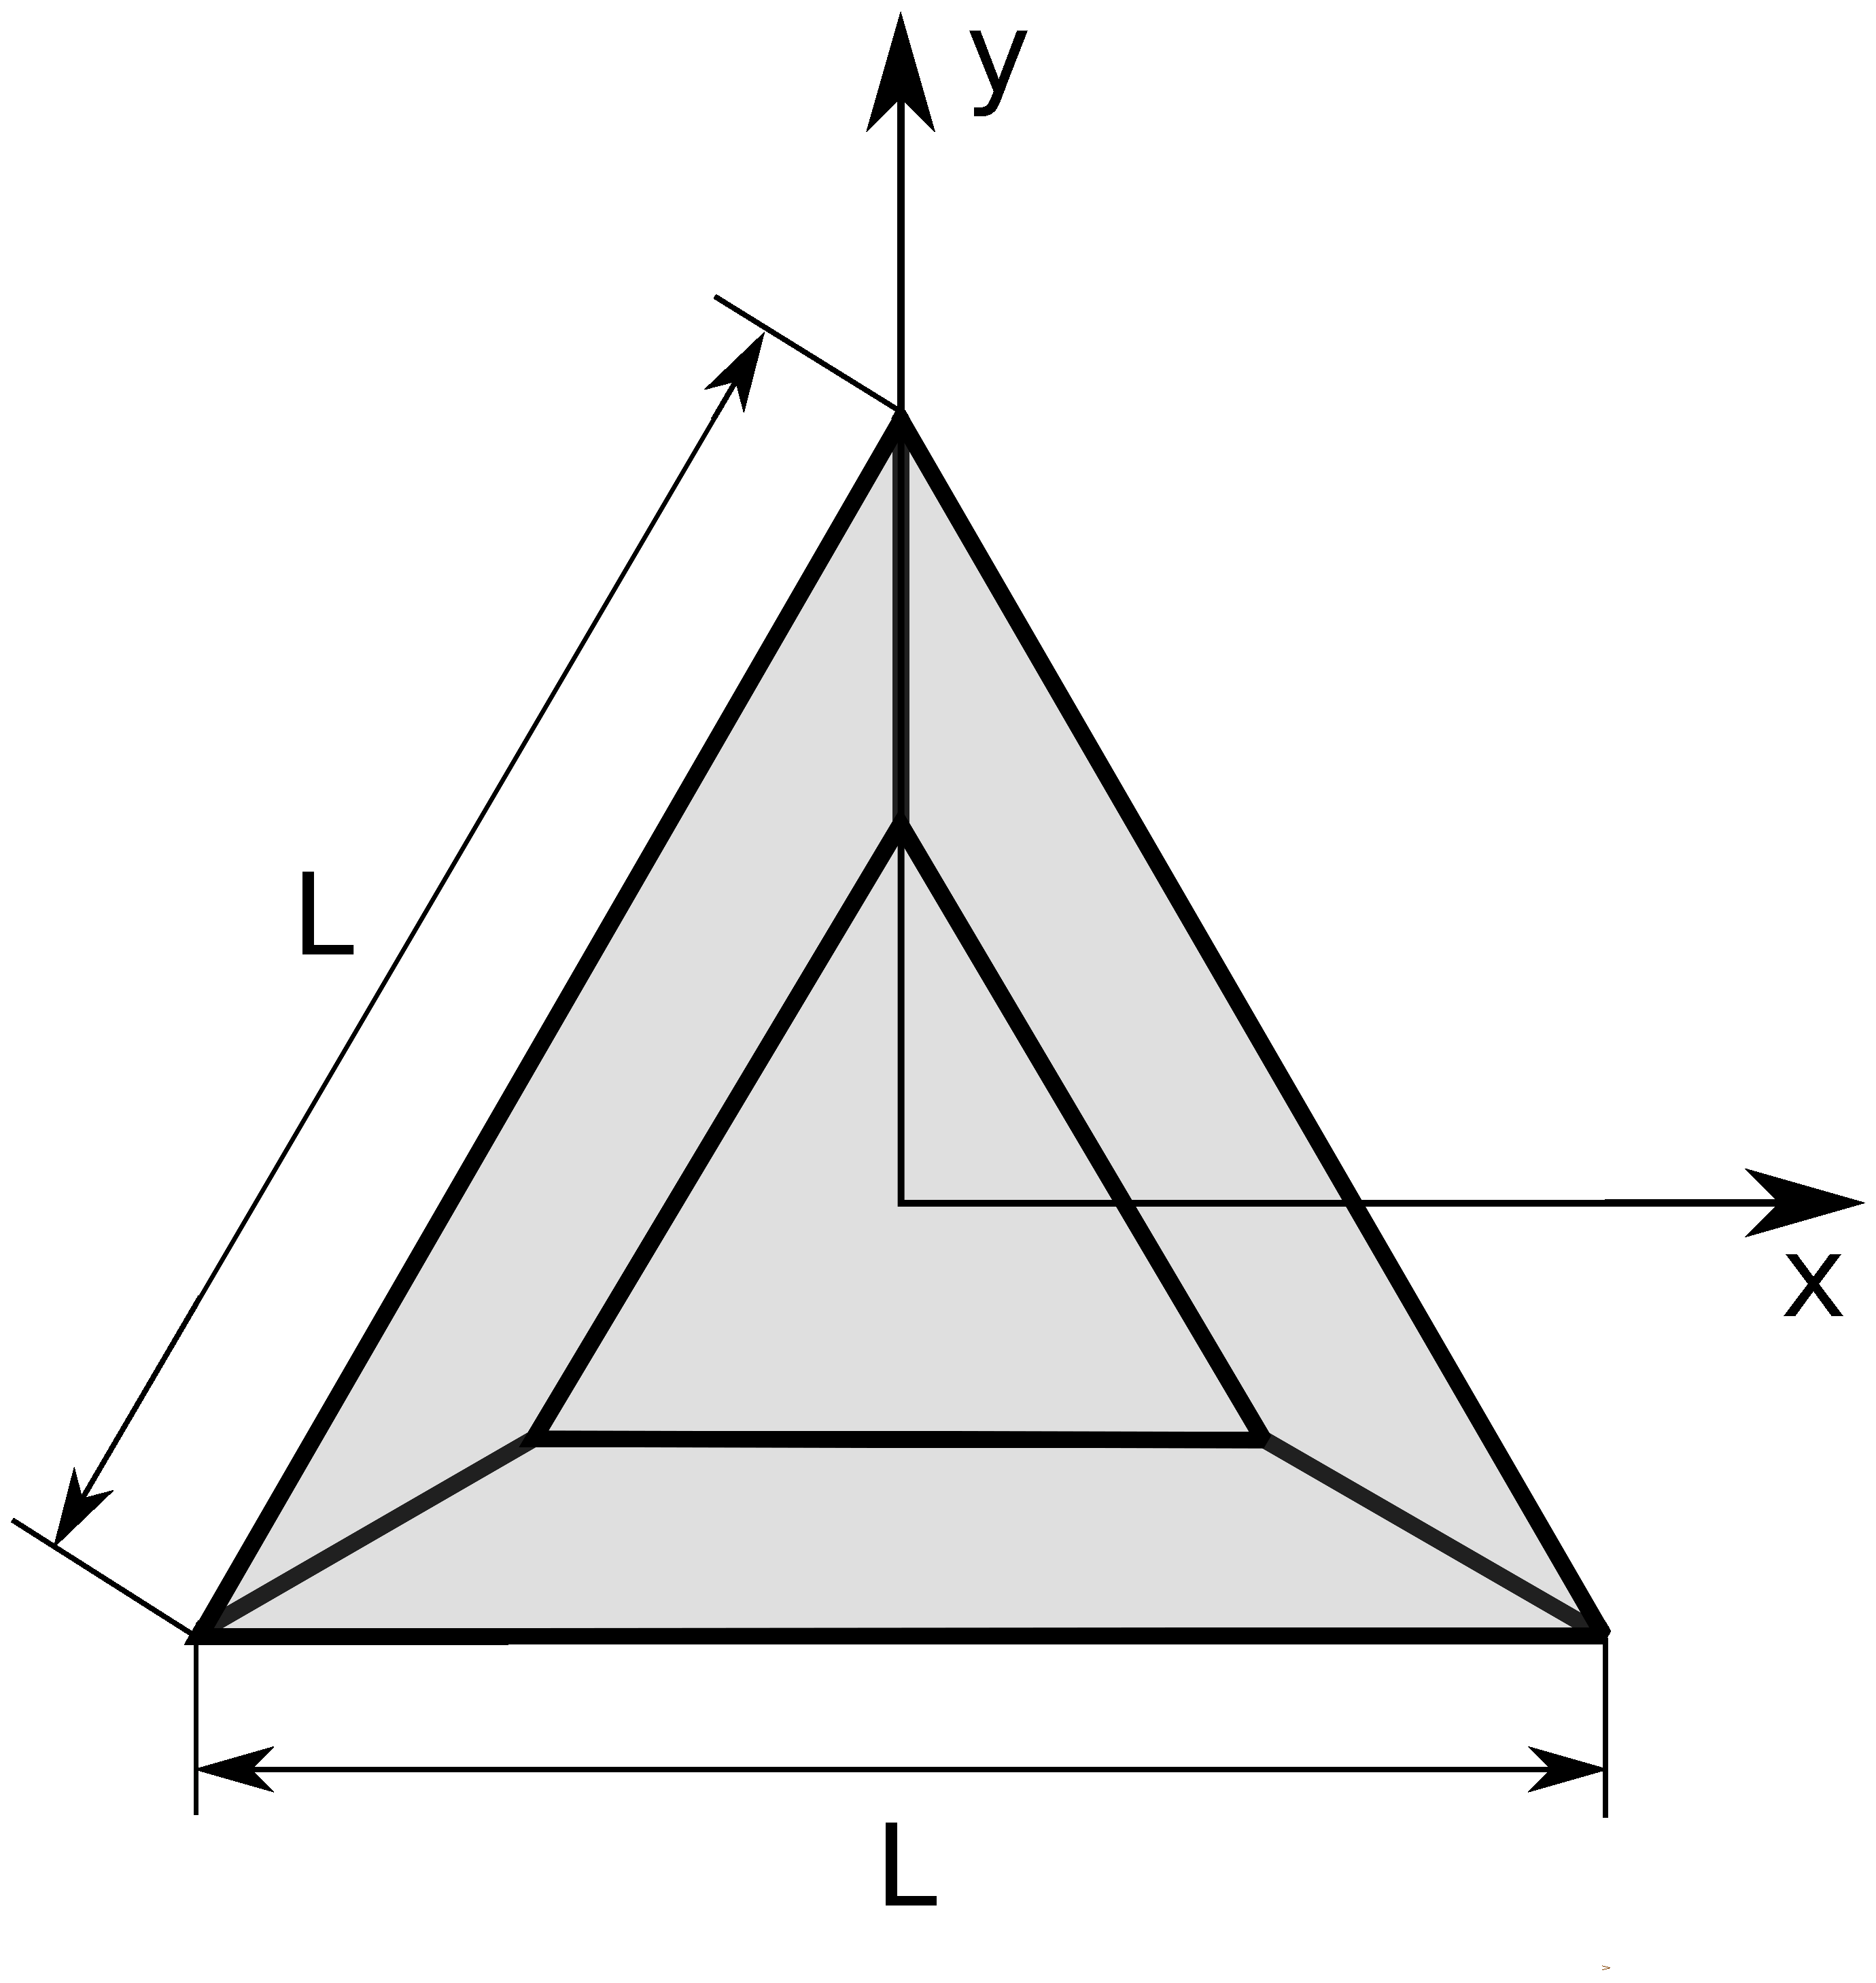
\includegraphics[width=5cm]{Figures/Tetrahedron2dxy}}
\hfill
\caption{Sketch of a Tetrahedron. The implementation of this shape uses angle
  $\alpha$, which is linked to $\beta$ via $\tan \alpha = 2 \tan 
  \beta$. $\alpha$ is measured along one of the base lines and $\beta$
  at one of the base vertices.}
\label{fig:tetrahedron}
\end{figure}

\FloatBarrier

\paragraph{Parameters:}
\begin{itemize}
\item length of one side of the equilateral triangular base $L$,
\item height $H$,
\item angle $\alpha$ is the angle between the base and the
  side faces, taken in the middle of the base lines.
\end{itemize}

\paragraph{Restrictions on the parameters:} $\dfrac{H}{L}< \dfrac{\tan{\alpha}}{2\sqrt{3}}$.

\paragraph{Properties:}
\begin{itemize}
\item volume $V= \dfrac{\tan(\alpha)}{24} L^3\Big[1- (1 -
  \sqrt{3}\dfrac{2H}{L \tan(\alpha)} )^3\Big]$,
\item particle surface seen from above $S =\dfrac{\sqrt{3}}{4}L^2$.
%\item radius of gyration
\end{itemize}

\subsection{Expression of the form factor}

\begin{align*}
&F_{\rm{Tetrahedron}} (\mathbf{q}, L, H, \alpha)=\frac{\sqrt{3}H}{q_x (q_x^2-3q_y^2)}
\exp\left(iq_z \frac{L}{2\tan (\alpha)\sqrt{3}}\right) \times \\
&\Big\{2q_x \exp(iq_3 D)\sinc(q_3 H) - (q_x +\sqrt{3}q_y)
\exp(iq_1 D)\sinc(q_1 D) -(q_x-\sqrt{3}q_y)\exp(-iq_2
D)\sinc(q_2 H) \Big\}, 
\end{align*}
with $\sinc(x)=\sin(x)/x$,
\begin{equation*}
q_1  =\frac{1}{2}\left[\frac{q_x\sqrt{3} -q_y}{\tan \alpha}-q_z \right],
\quad q_2 = \frac{1}{2}\left[\frac{q_x\sqrt{3} +q_y}{\tan \alpha}+q_z
\right], \quad 
q_3 = \frac{q_y}{\tan \alpha} -\frac{q_z}{2}, \quad D = \frac{L \tan \alpha}{\sqrt{3}} -H.
\end{equation*}

\paragraph{Syntax:} \Code{FormFactorTetrahedron(length, height, alpha)}

\subsection{Examples}
Figure~\ref{fig:FFtetrahEx} shows the normalized intensity
$|F|^2/V^2$, computed with $L=15$~nm, $H=6$~nm and $\alpha =60
^{\circ}$.

\begin{figure}[h]
\begin{center}
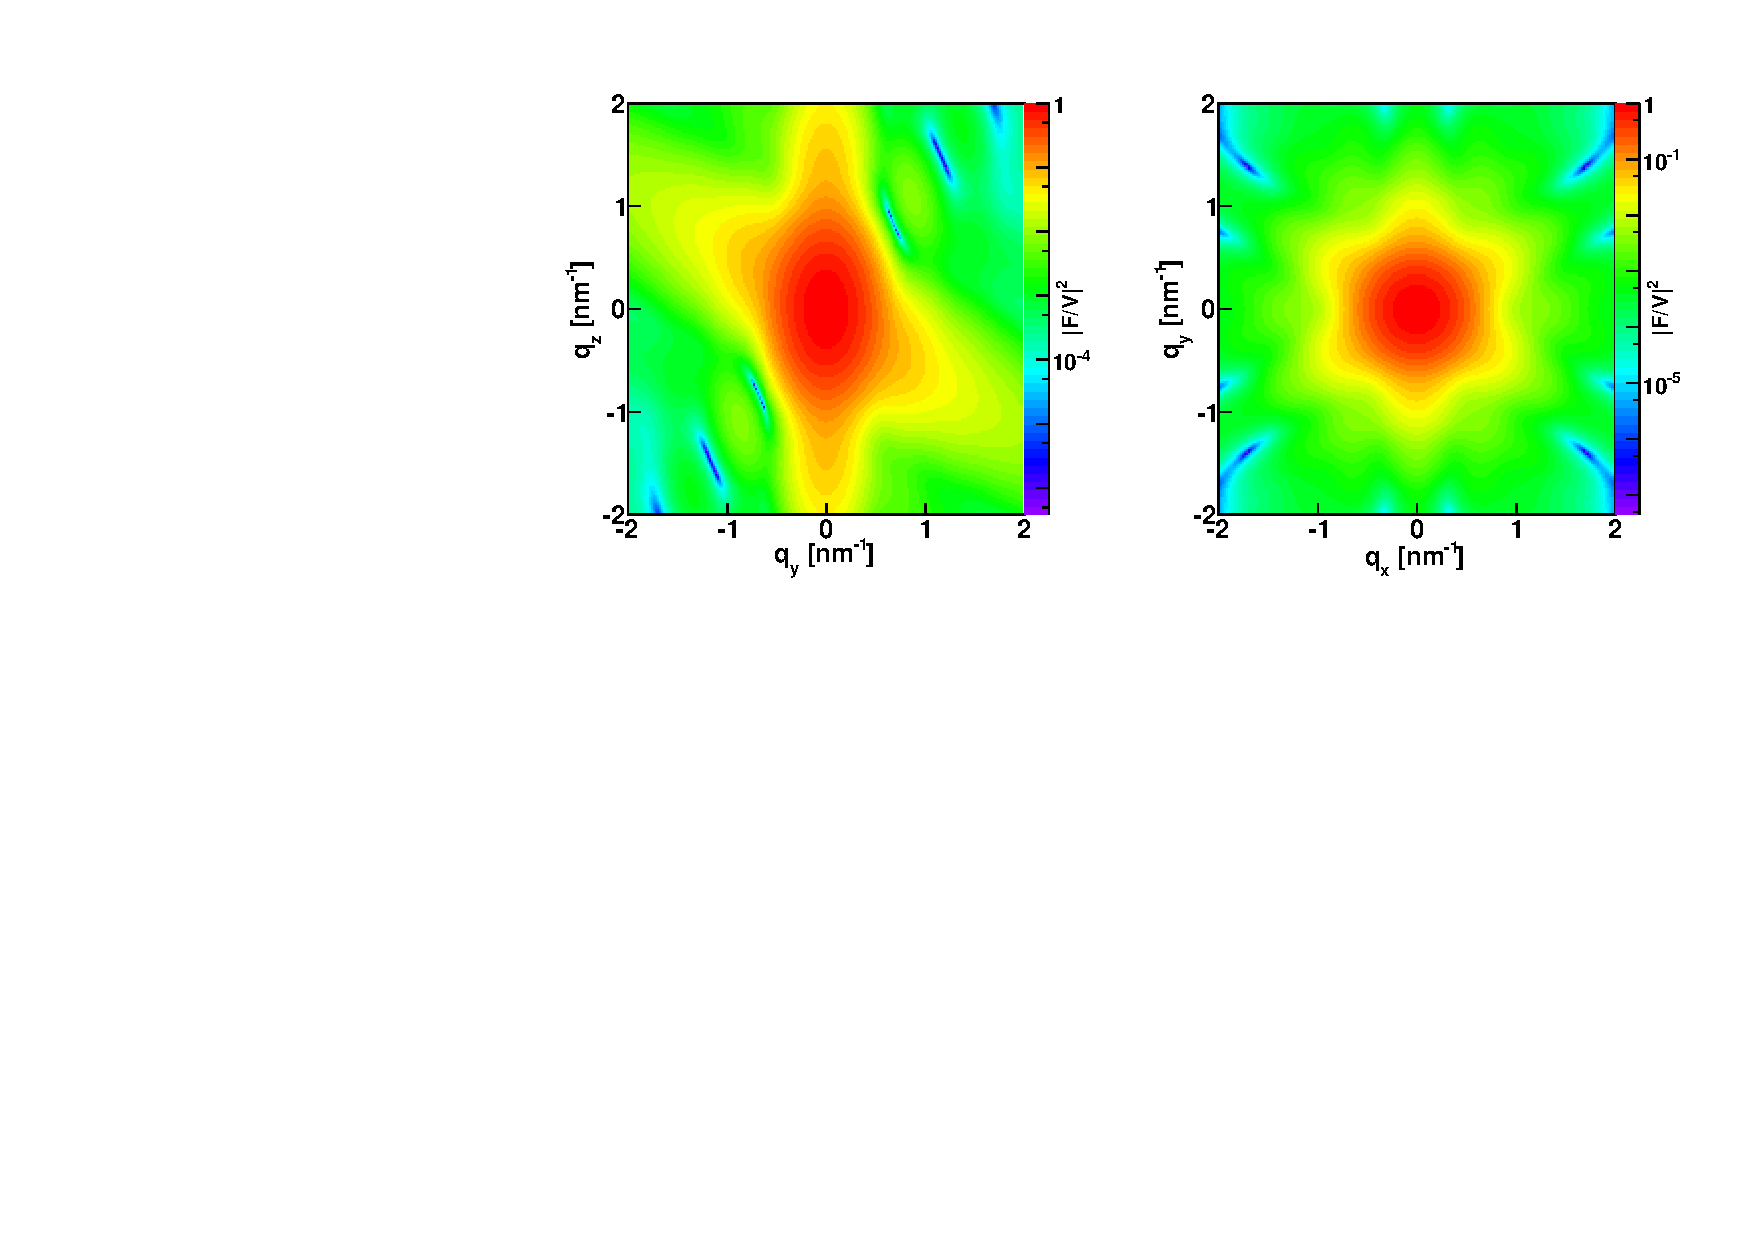
\includegraphics[width=\textwidth]{Figures/figfftetrahedron}
\end{center}
\caption{Normalized intensity for the form factor of a Tetrahedron
  $|F|^2/V^2$, plotted against ($q_z$, $q_y$) and  ($q_x$, $q_y$) and
  computed with $L=15$~nm, $H=6$~nm and $\alpha=60^{\circ}$.}
\label{fig:FFtetrahEx}
\end{figure}

\FloatBarrier

%\subsection{References}
%In \Code{IsGISAXS}, factor 1/sqrt(3) instead of sqrt(3) in the
%expression of the form factor. When running the software, there is
%also a problem with this form factor.
%In the $x,y$ plane , we use the full side length of the triangular
%base instead of  half as implemented in \Code{IsGISAXS}: $L= 2
%R_{\rm{\Code{IsGISAXS}}}$.

\newpage{\cleardoublepage}
%%%%%%%%%%%%%%%%%%%%%%%%%%%%%%%%%%%%
\section{Prism6} \SecLabel{Prism6}

\subsection{Real-space geometry}
This shape is an hexagonal prism (see fig.~\ref{fig:prism6}).

\begin{figure}[ht]
\hfill
\subfigure[Side view]{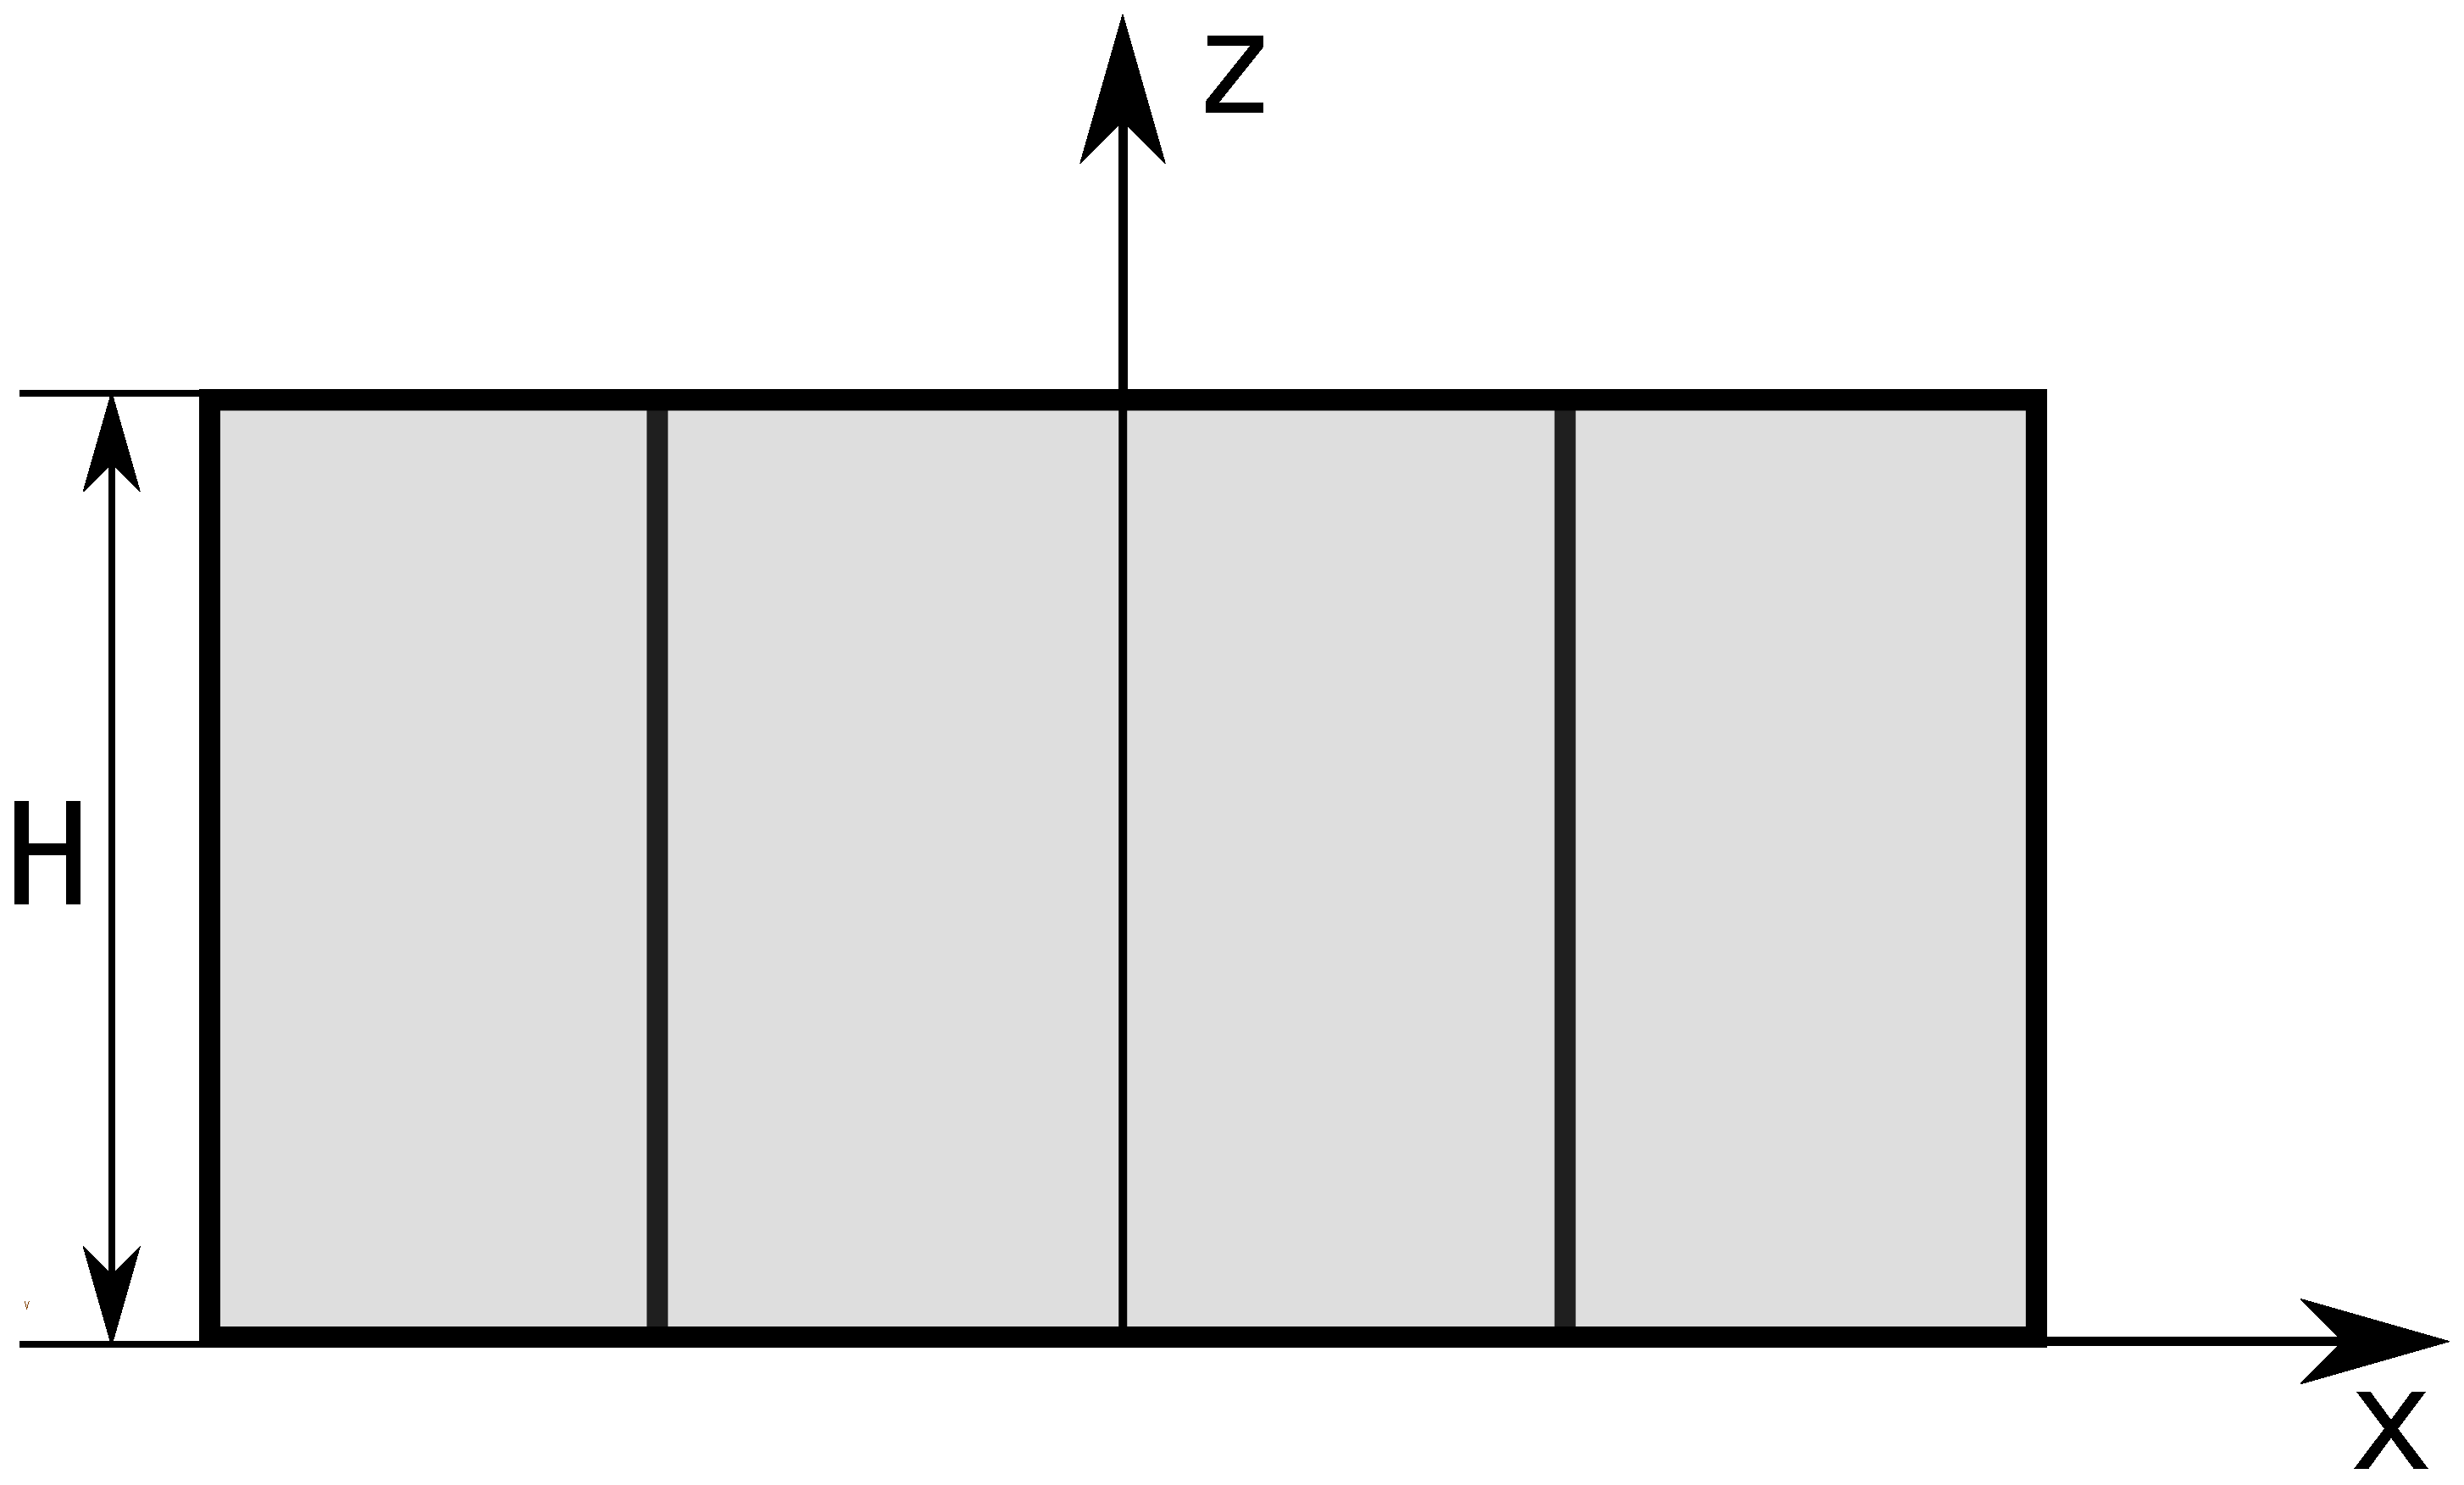
\includegraphics[width=5cm]{Figures/Prism62dxz}}
\hfill
\subfigure[Top view]{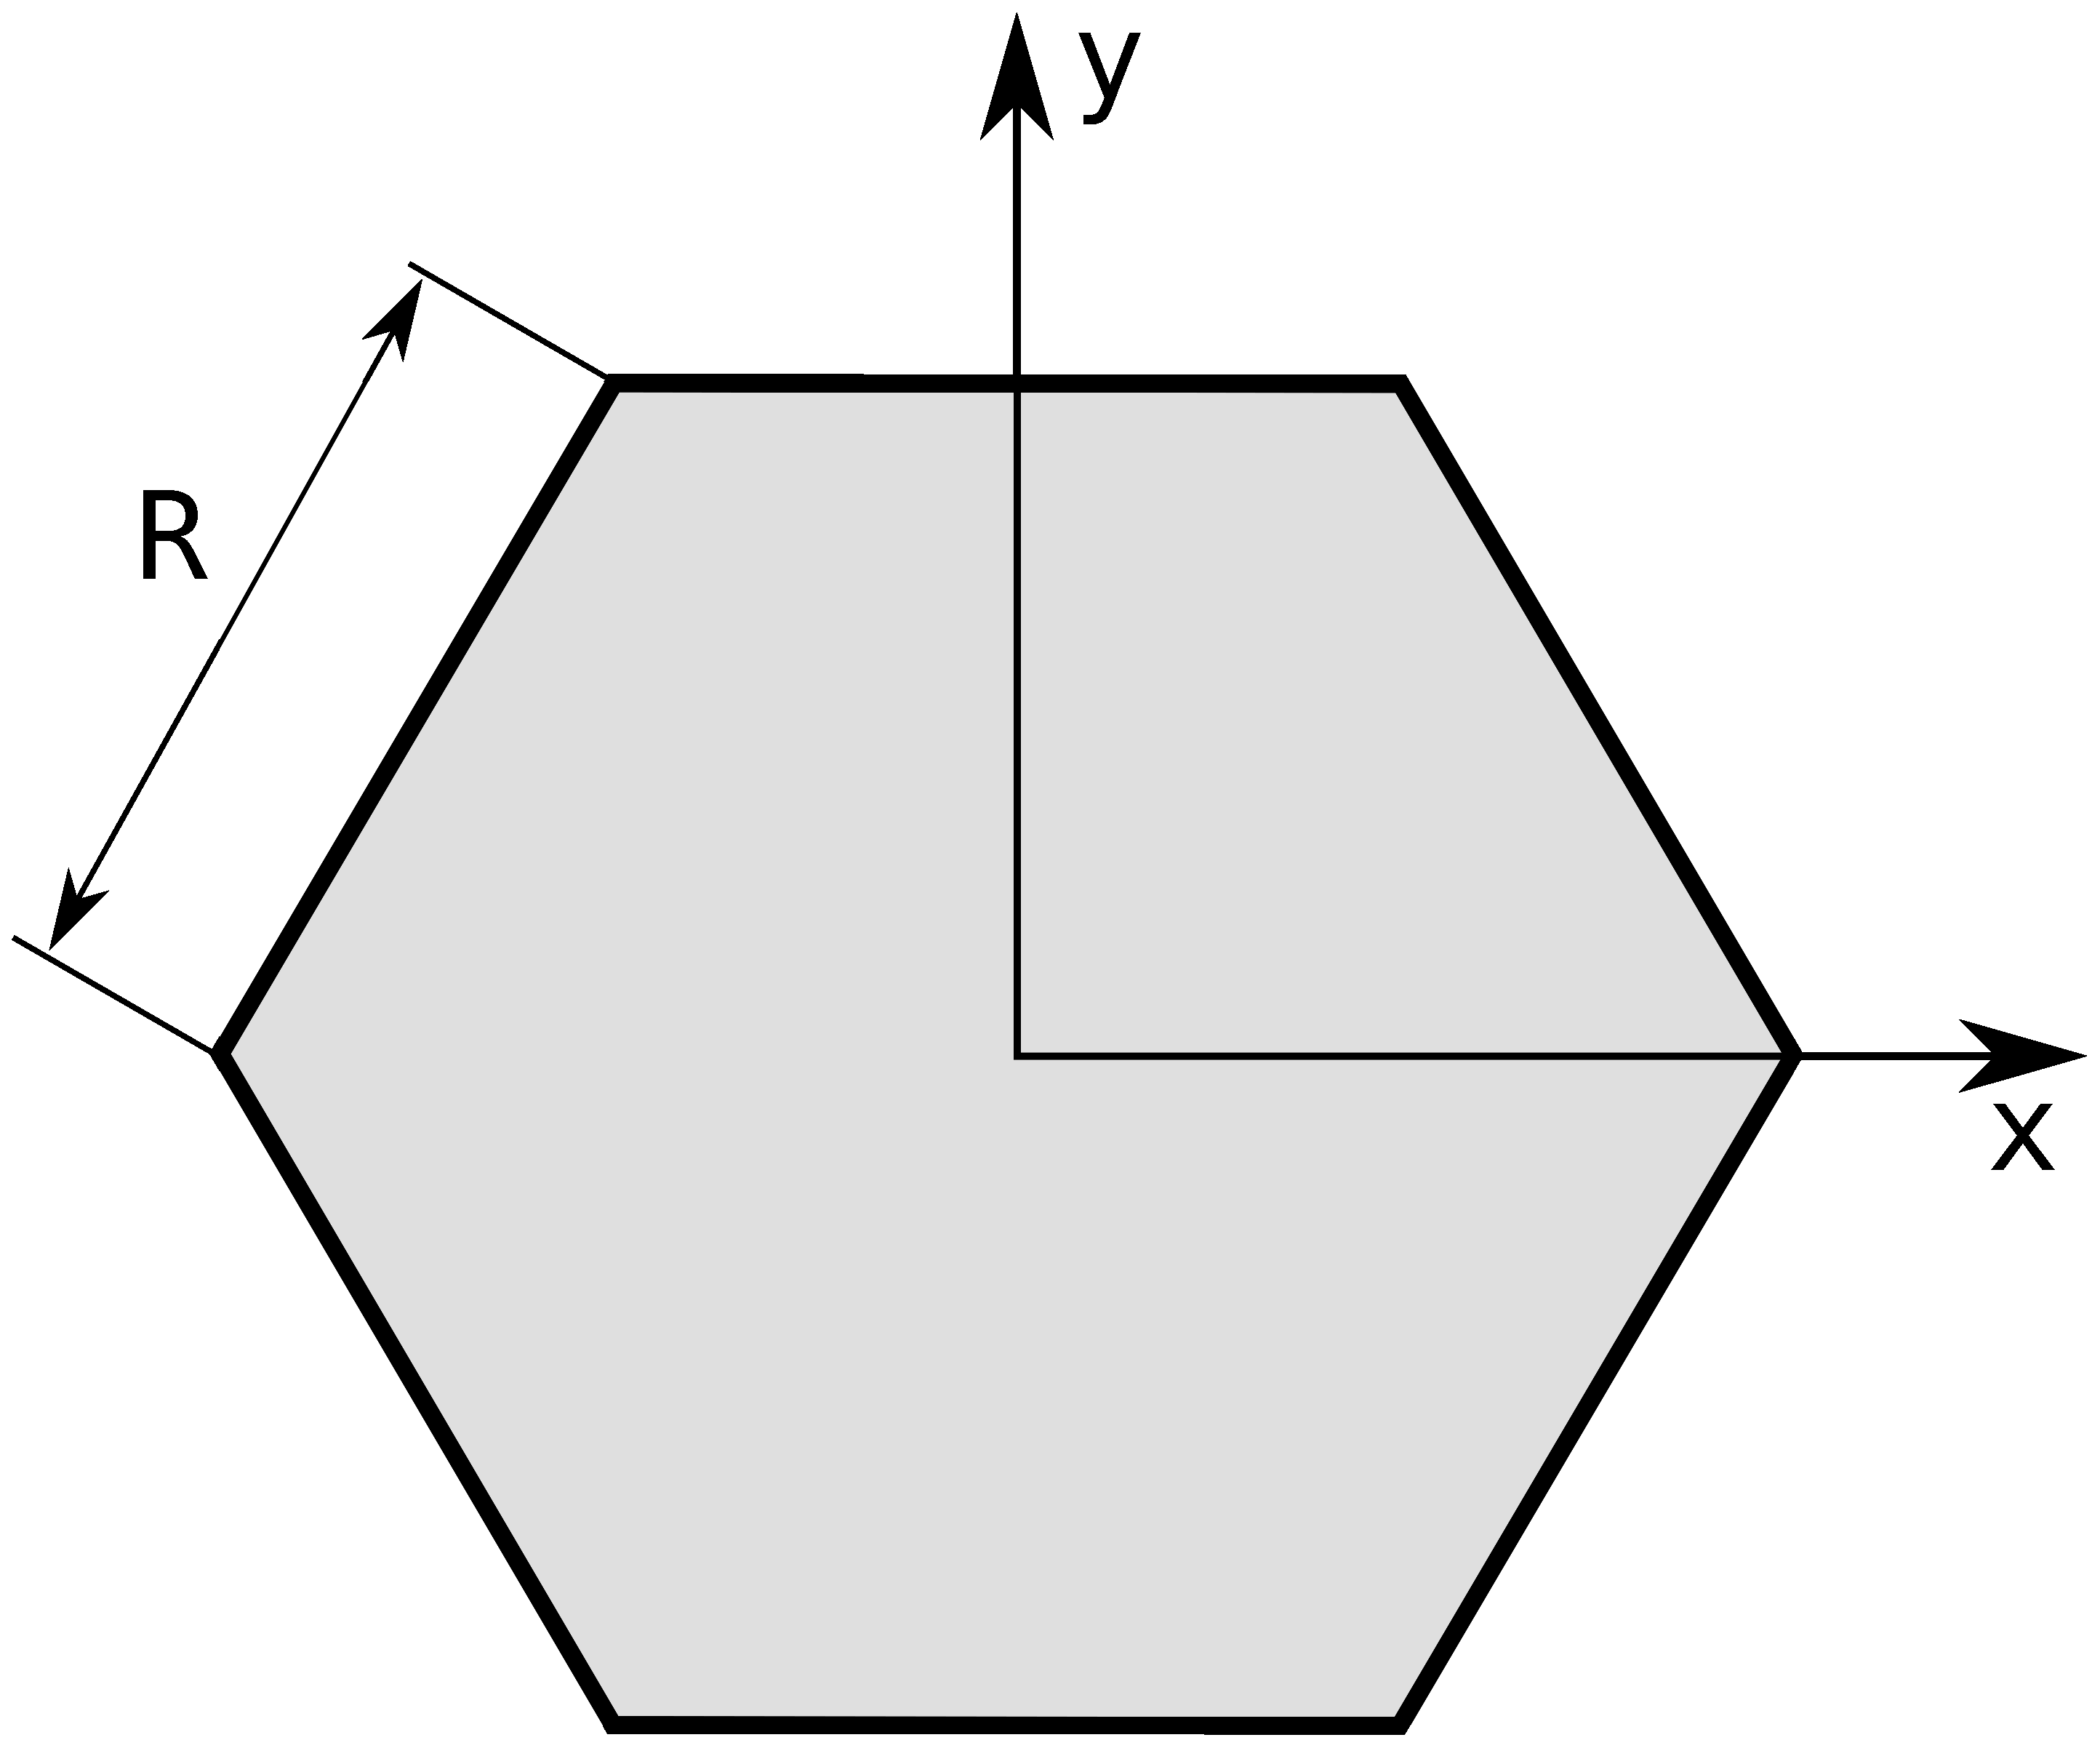
\includegraphics[width=5cm]{Figures/Prism62dxy}}
\hfill
\caption{Sketch of a Prism6.}
\label{fig:prism6}
\end{figure}

\FloatBarrier

\paragraph{Parameters:}
\begin{itemize}
\item radius of the hexagonal base $R$,
\item height $H$.
\end{itemize}

\paragraph{Properties:}
\begin{itemize}
\item volume $V = \dfrac{3\sqrt{3}}{2}H R^2$,
\item particle surface seen from above $S =\dfrac{3\sqrt{3}R^2}{2}$.
%\item radius of gyration.
\end{itemize}

\subsection{Expression of the form factor}
\begin{align*}
F_{\rm{Prism6}}(\mathbf{q}, R, H) &= \frac{4H\sqrt{3}}{3q_y^2 - q_x^2}
\sinc\left(q_z\frac{H}{2}\right) \exp\left(-i q_z\frac{ H}{2}\right)\times\\
&\left\{\frac{3q_y^2R^2}{4} \sinc\left(\frac{q_x
  R}{2}\right)\sinc\left(\frac{\sqrt{3}q_yR }{2}\right)+ \cos(q_x R)-\cos\left(q_y
\frac{\sqrt{3}R}{2}\right) \cos\left(\frac{q_x R}{2}\right)\right\},
\end{align*}
with $\sinc(x)=\sin(x)/x$.

\paragraph{Syntax:} \Code{FormFactorPrism6(radius, height)} 

\subsection{Examples}
Figure~\ref{fig:FFprism6Ex} shows the normalized intensity
$|F|^2/V^2$, computed with $R=5$~nm and \mbox{$H=11$~nm.}

\begin{figure}[h]
\begin{center}
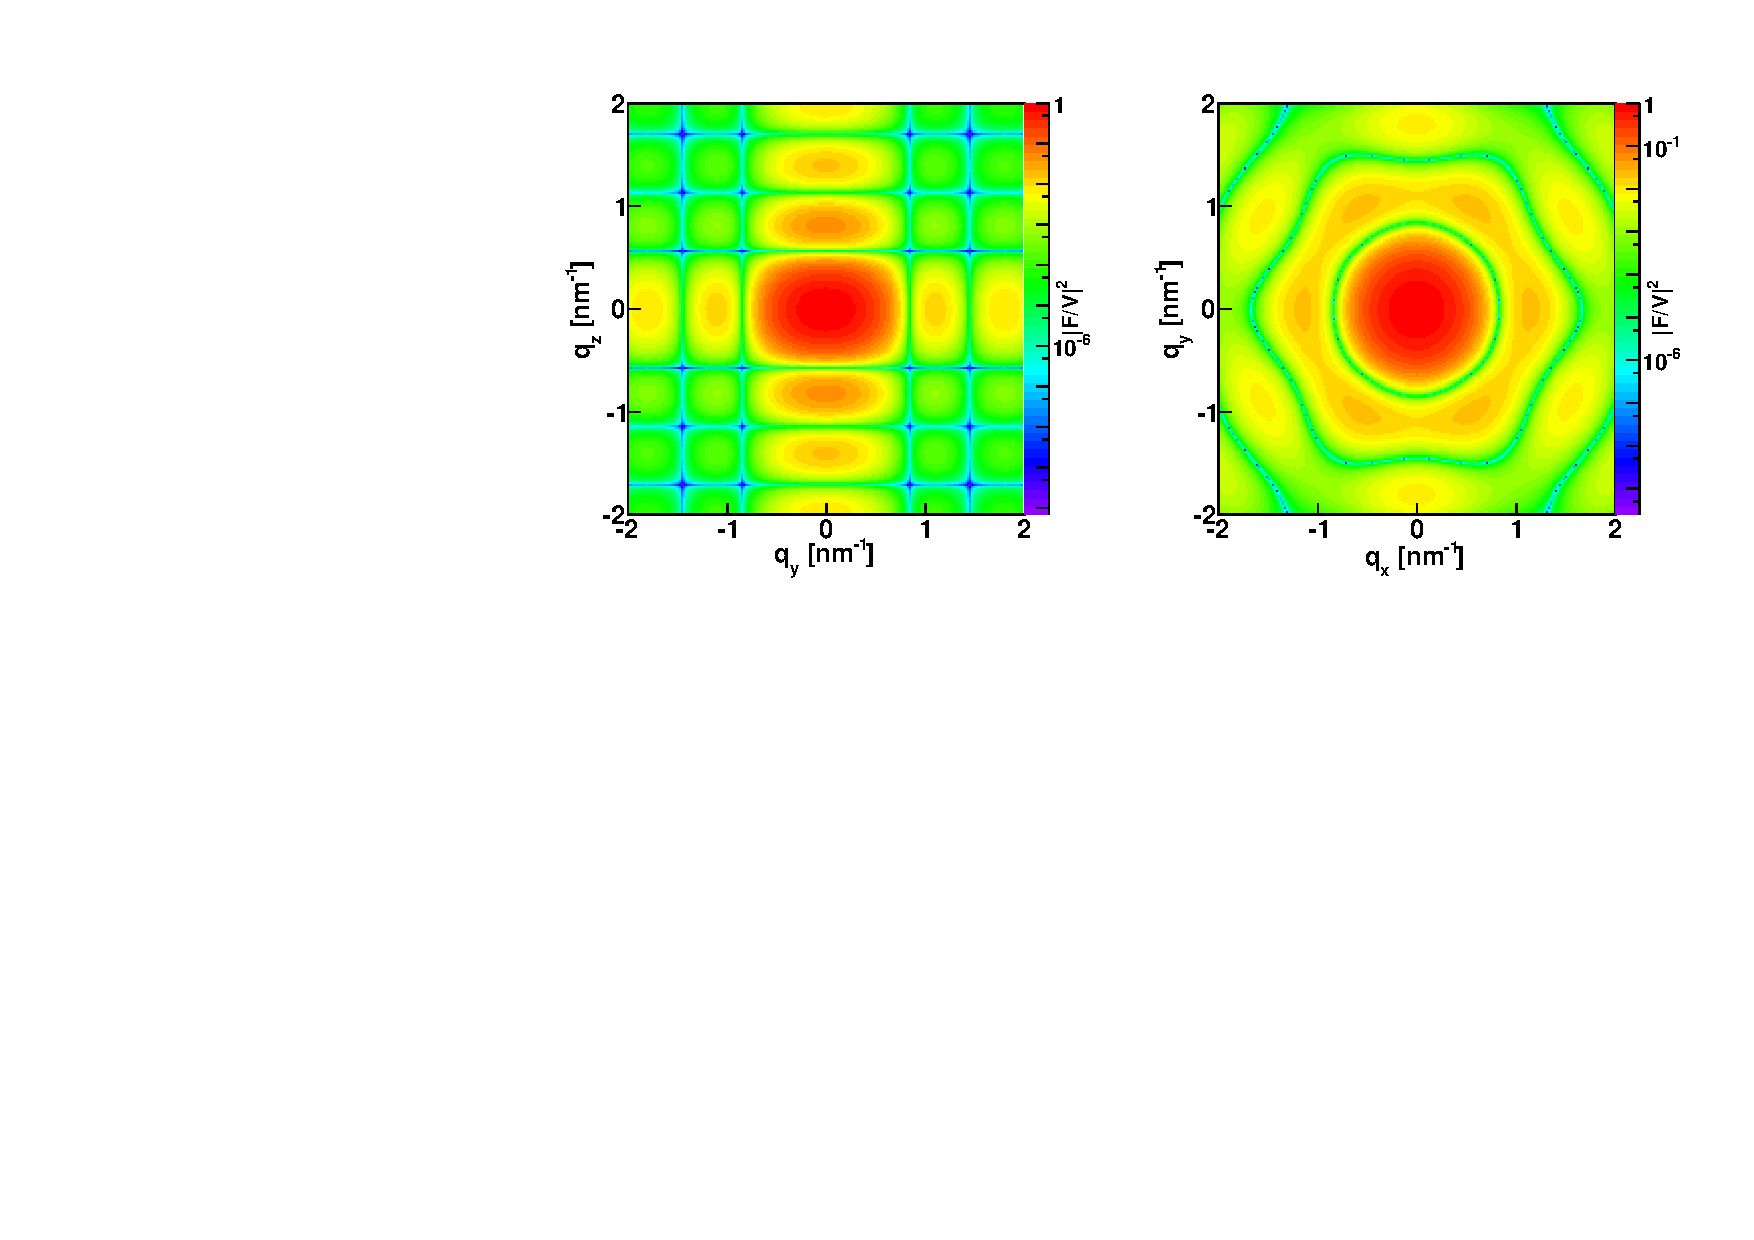
\includegraphics[width=\textwidth]{Figures/figffprism6}
\end{center}
\caption{Normalized intensity for the form factor of a Prism6
  $|F|^2/V^2$, plotted against ($q_z$, $q_y$) and ($q_x$, $q_y$) and computed with $R=5$~nm and $H=11$~nm.}
\label{fig:FFprism6Ex}
\end{figure}

\FloatBarrier

%\subsection{References}
%The hexagonal base is parametrized in the different way compared with
%\Code{IsGISXAXS}. In \BornAgain\, we use $R = 2/\sqrt{3}R_{\text{\Code{IsGiSaXs}}}$.
%A factor $H$ is missing in the expression of the form factor given in
%\Code{IsGISAXS}'s manual. 

\newpage{\cleardoublepage}
%%%%%%%%%%%%%%%%%%%%%%%%%%%%%%%%%%%%
\section{Cone6} \SecLabel{Cone6} 

\subsection{Real-space geometry}
It is a truncated hexagonal pyramid (see fig.~\ref{fig:cone6}). 

\begin{figure}[ht]
\hfill
\subfigure[Side view]{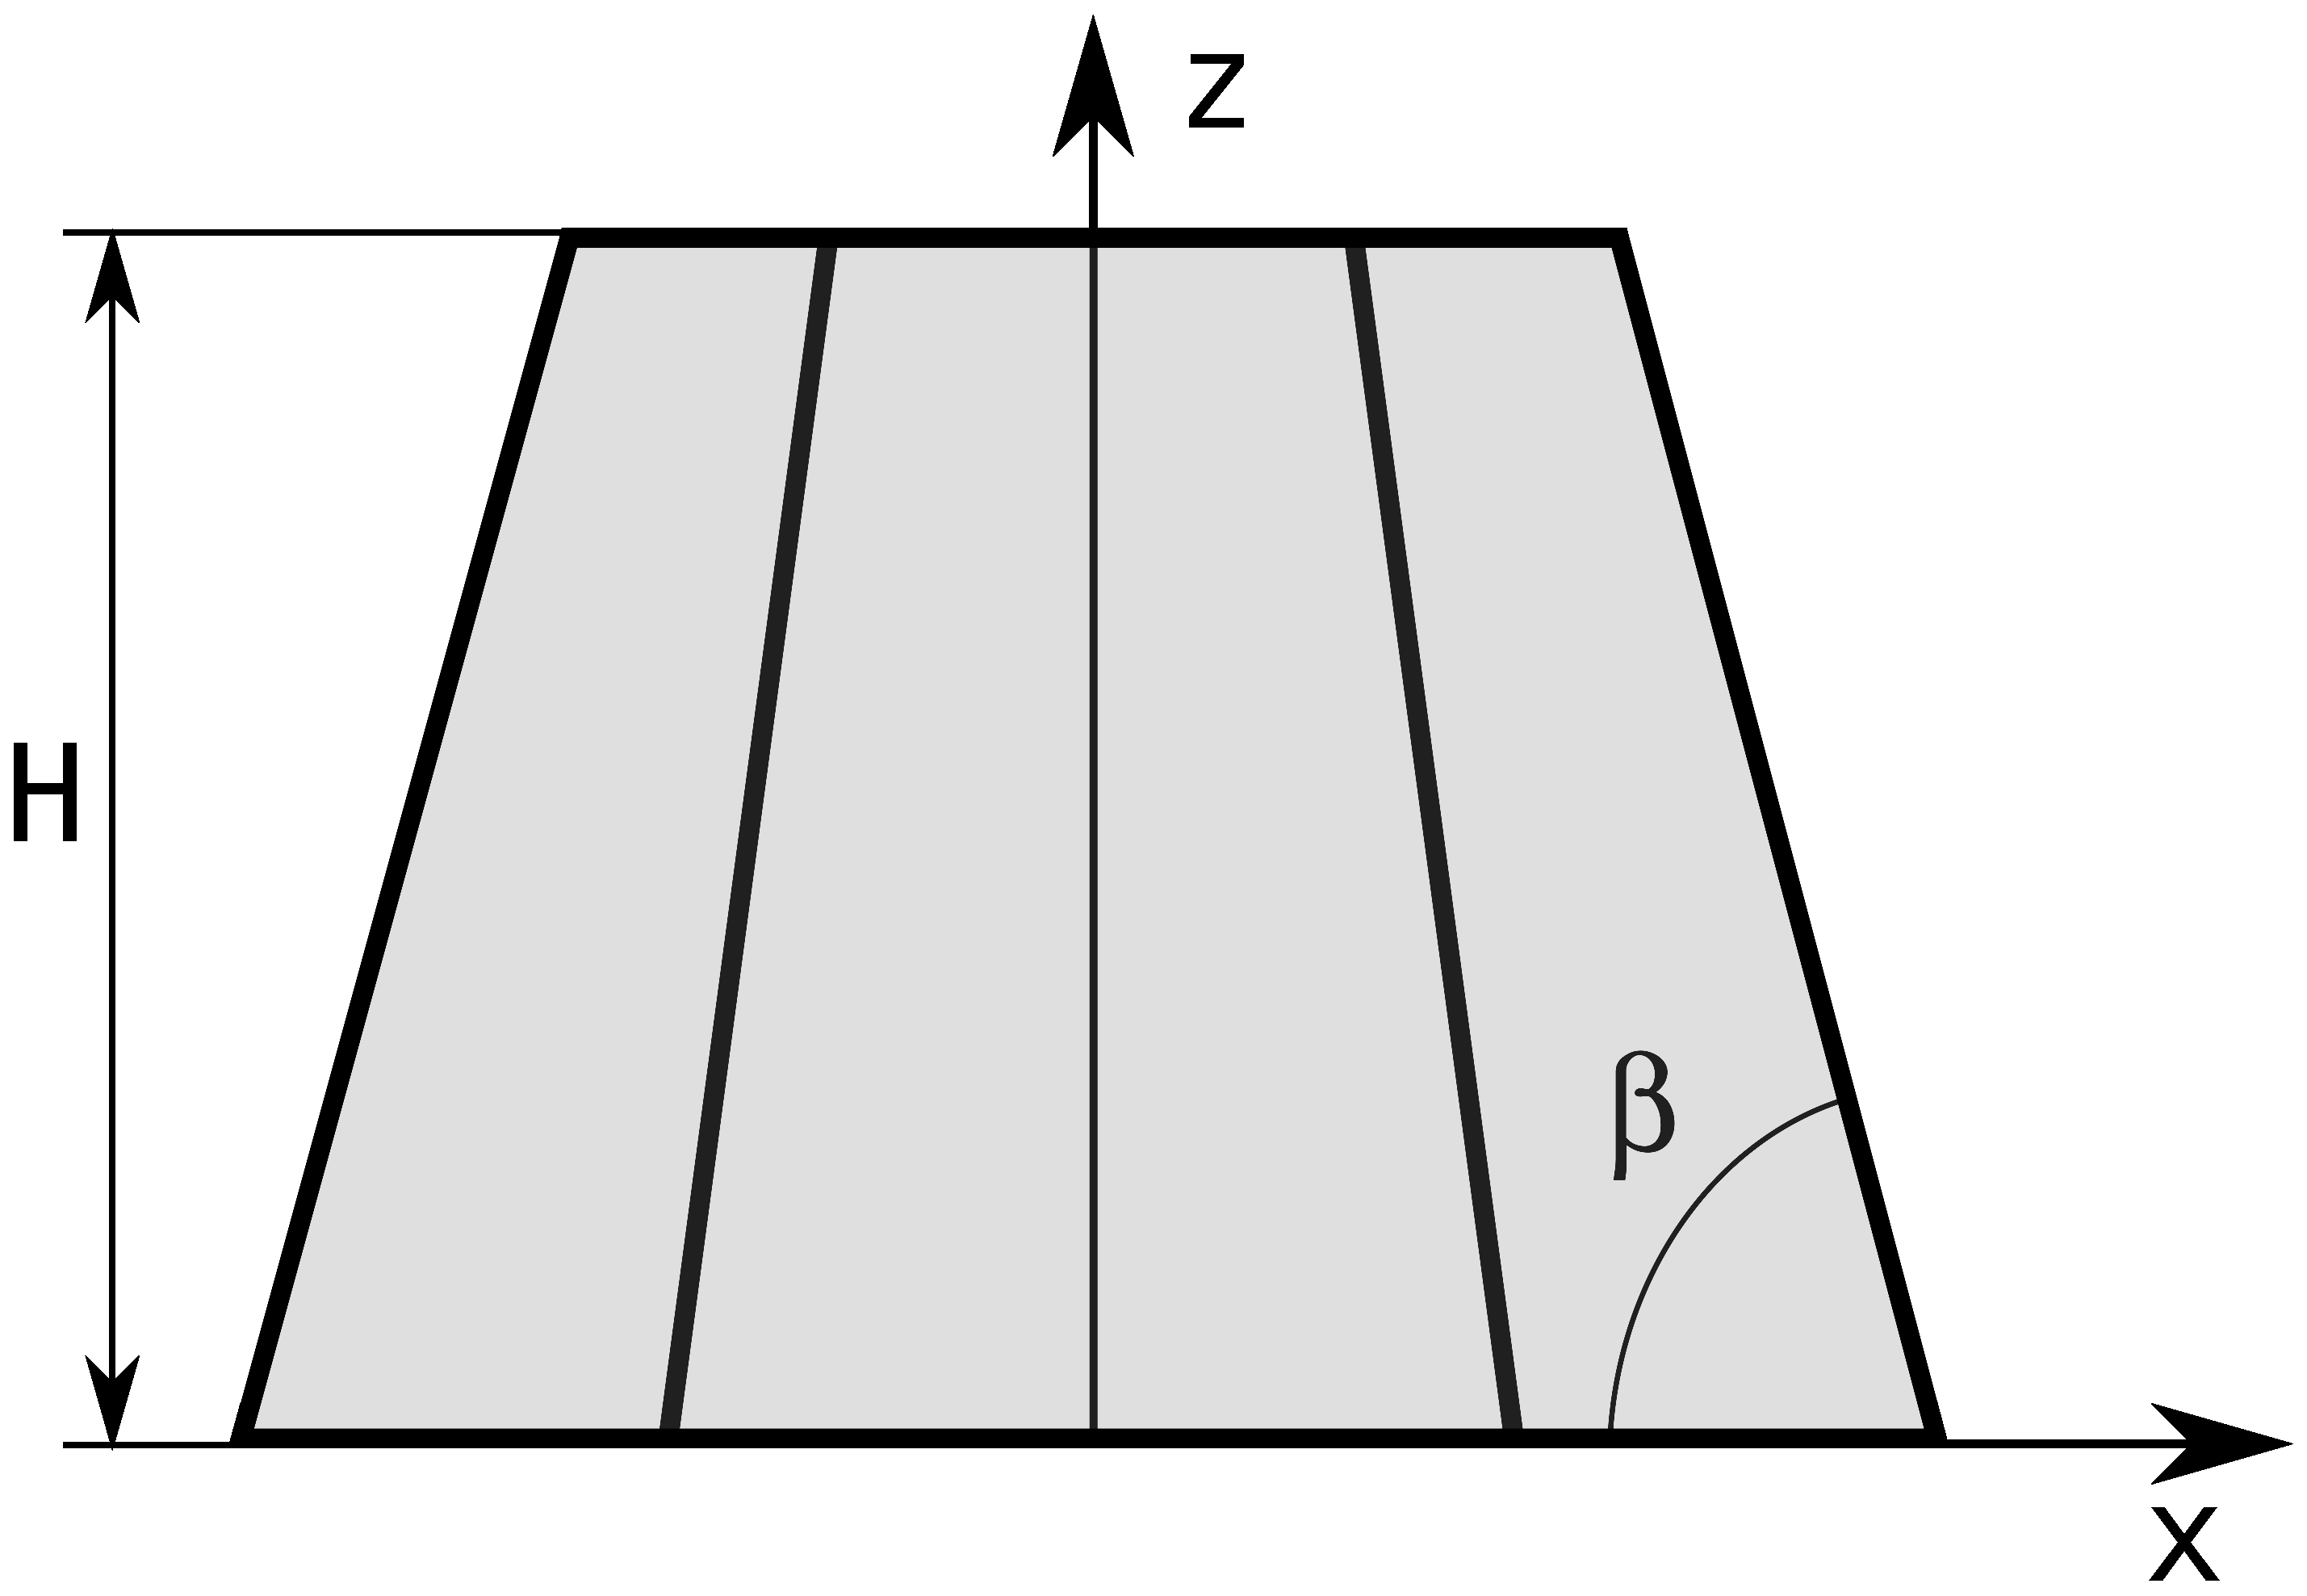
\includegraphics[width=5cm]{Figures/Cone62dxz}}
\hfill
\subfigure[Top view]{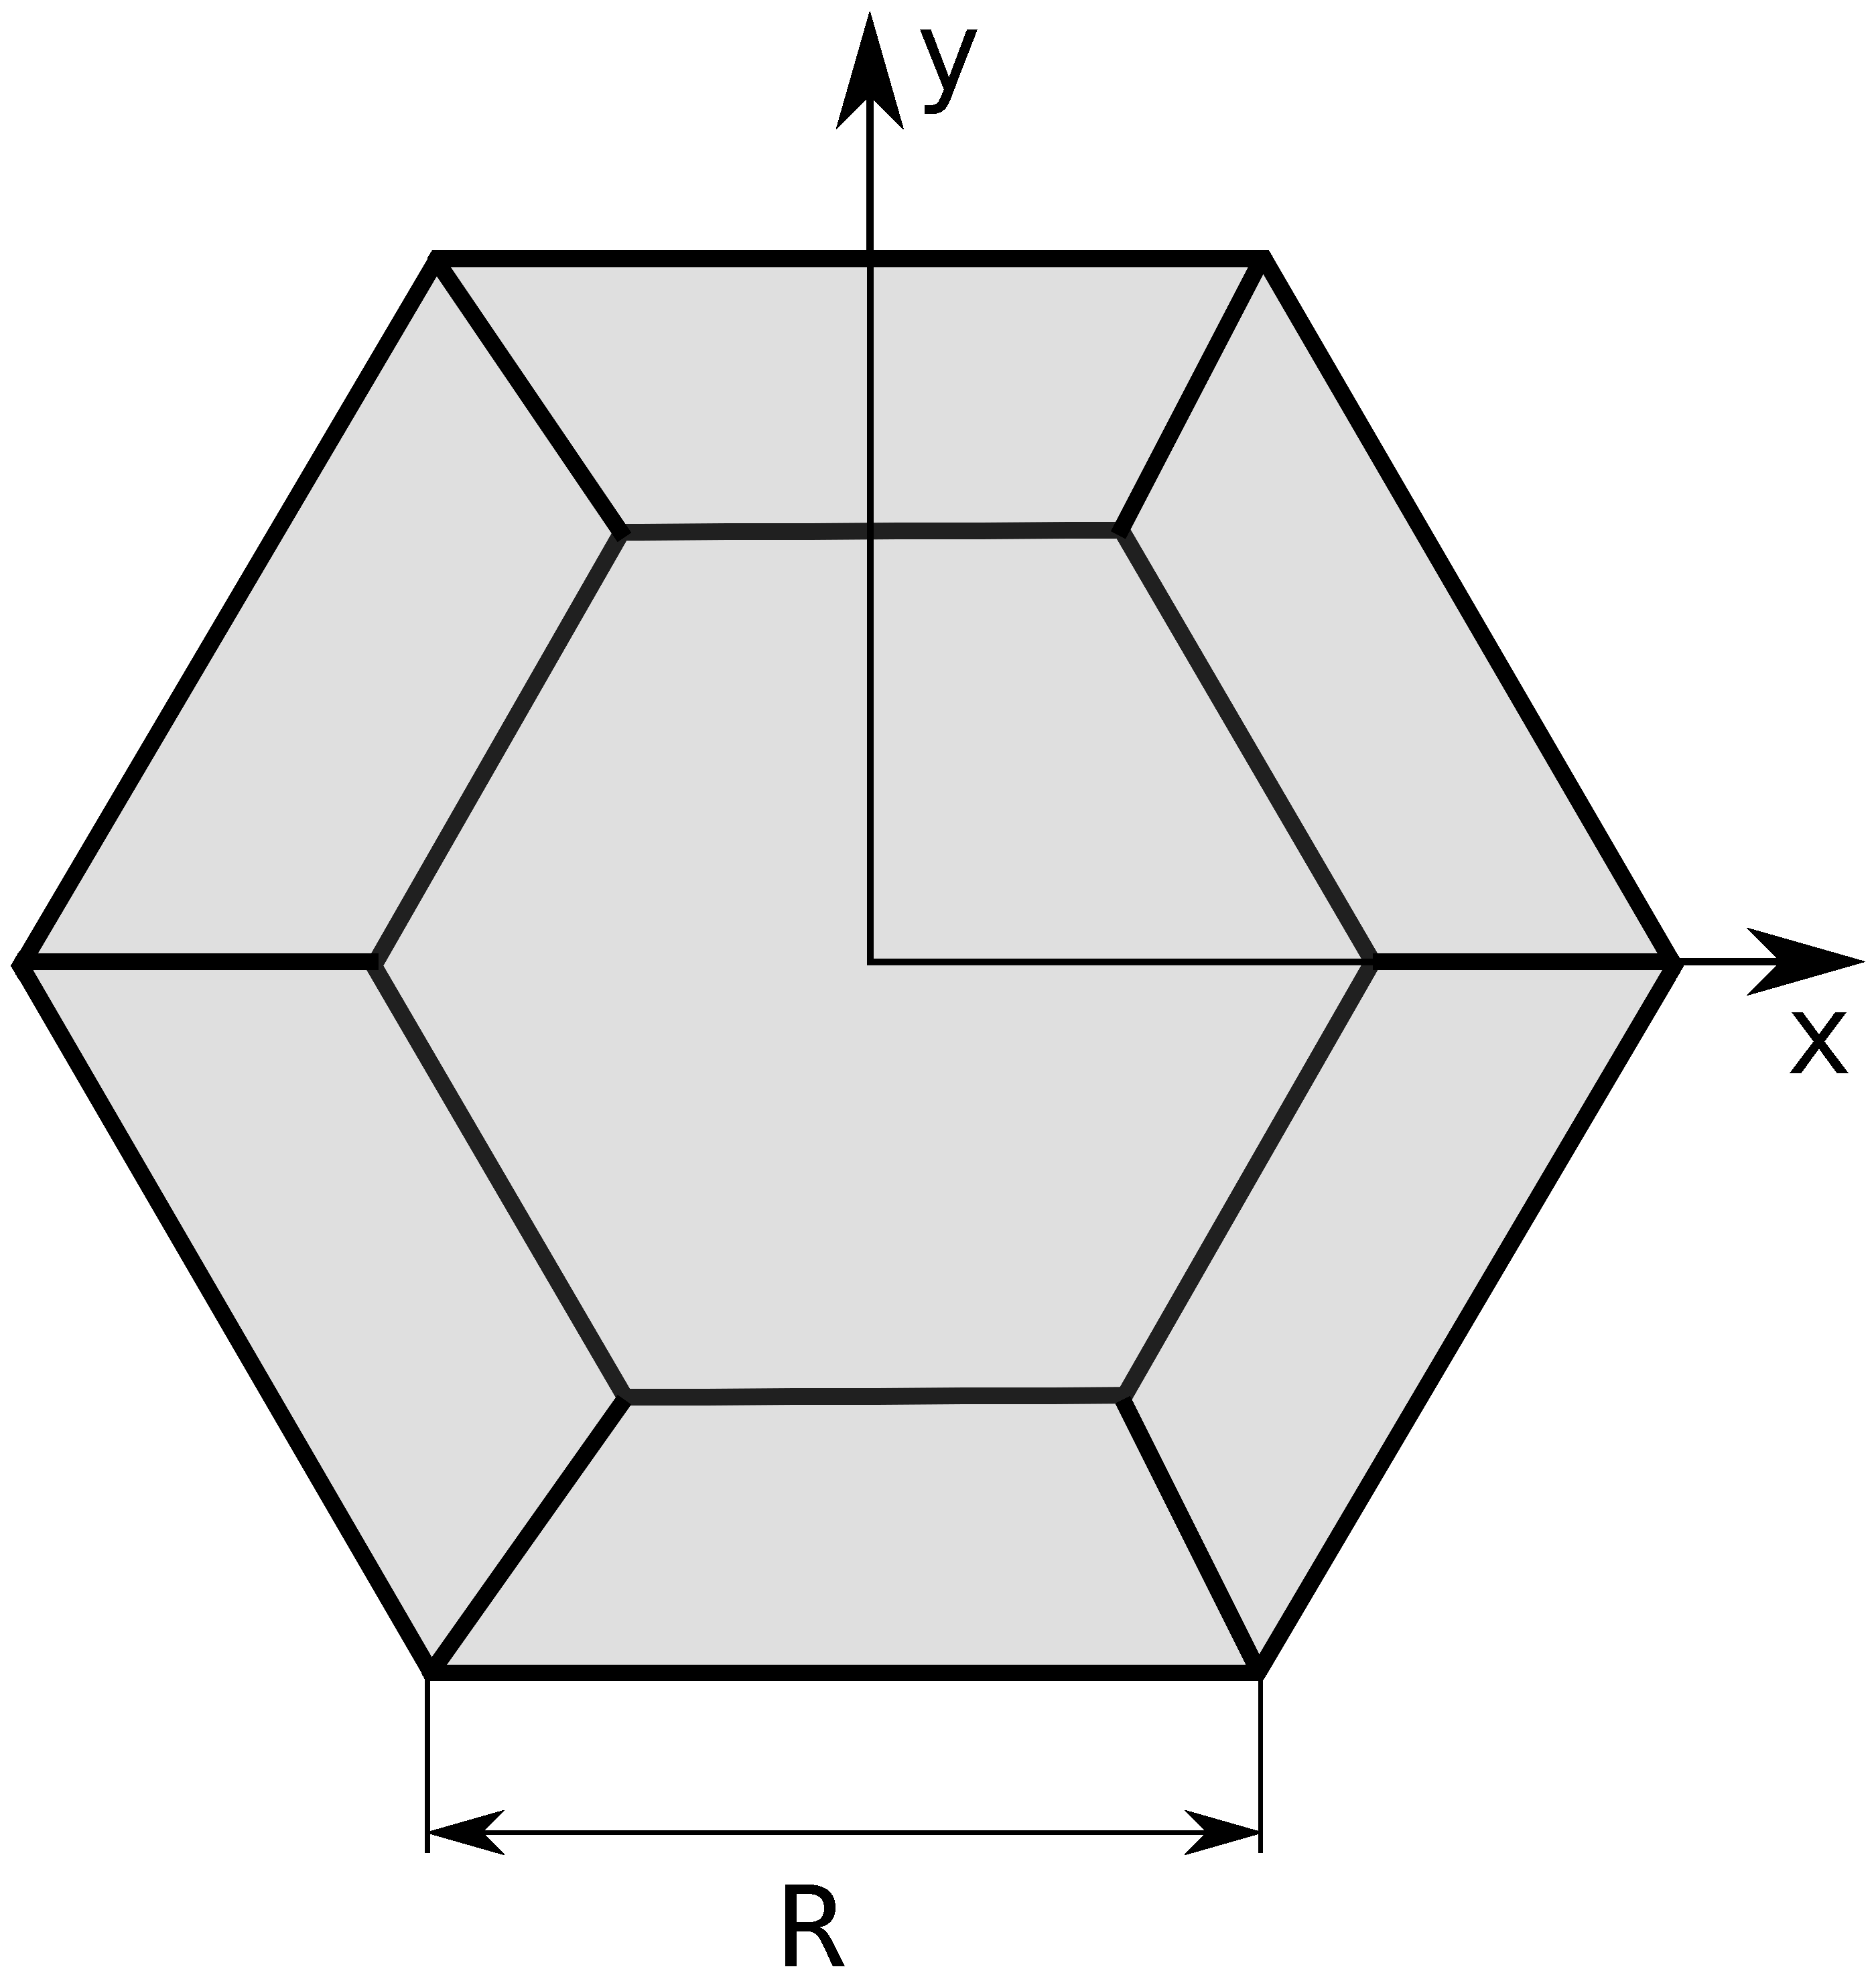
\includegraphics[width=5cm]{Figures/Cone62dxy}}
\hfill
\caption{Sketch of a Cone6.  The implementation of this shape uses angle
  $\alpha$, which is linked to $\beta$ via $\tan \alpha = \dfrac{2}{\sqrt{3}} \tan 
  \beta$. $\alpha$ is measured along one of the base lines and $\beta$
  at one of the base vertices.}
\label{fig:cone6}
\end{figure}

\FloatBarrier


\paragraph{Parameters:}
\begin{itemize}
\item radius of the regular hexagonal base $R$,
\item height $H$,
\item angle $\alpha$ is considered between one of the side faces and
  the middle of a base length. 
\end{itemize}

\paragraph{Restrictions on the parameters:} $\dfrac{2H}{\sqrt{3}R}< \tan{\alpha}$.

\paragraph{Properties:}
\begin{itemize}
\item volume $V = \dfrac{3}{4} \tan(\alpha) R^3 \Big[
            1 - \big(1- \dfrac{2H}{ \tan(\alpha) R\sqrt{3}}\big)^3
            \Big]$,
\item  particle surface seen from above $S =\dfrac{3\sqrt{3}R^2}{2}$.
%\item radius of gyration
\end{itemize}

\subsection{Expression of the form factor}
The
calculation can be derived from ``Prism6'' (\SecRef{Prism6}) by
considering a side length varying with the vertical position:

\begin{align*}
F_{\rm{Cone6}}(\mathbf{q}, R, H, \alpha) &= \frac{4\sqrt{3}}{3q_y ^2 - q_x^2}\int_0 ^H \exp(iq_z z)
\Big[\frac{3}{4}R_z^2q_y^2 \sinc\left(\frac{q_xR_z}{2}\right)\sinc\left(\frac{\sqrt{3}q_y
R_z}{2}\right)\\
&+\cos(q_xR_z)-\cos\left(\frac{\sqrt{3}q_y R_z}{2}\right)\cos\left(\frac{q_xR_z}{2}\right) \Big]dz
\end{align*}
with $R_z=R-\dfrac{2z}{\sqrt{3}\tan(\alpha)}$ and $\sinc(x)=\sin(x)/x$.

\paragraph{Syntax:} \Code{FormFactorCone6(radius,height, alpha)} 

\subsection{Examples}
Figure~\ref{fig:FFCone6Ex} shows the normalized intensity
$|F|^2/V^2$, computed with $R=10$~nm, $H=13$~nm, and
$\alpha=60^{\circ}$.

\begin{figure}[h]
\begin{center}
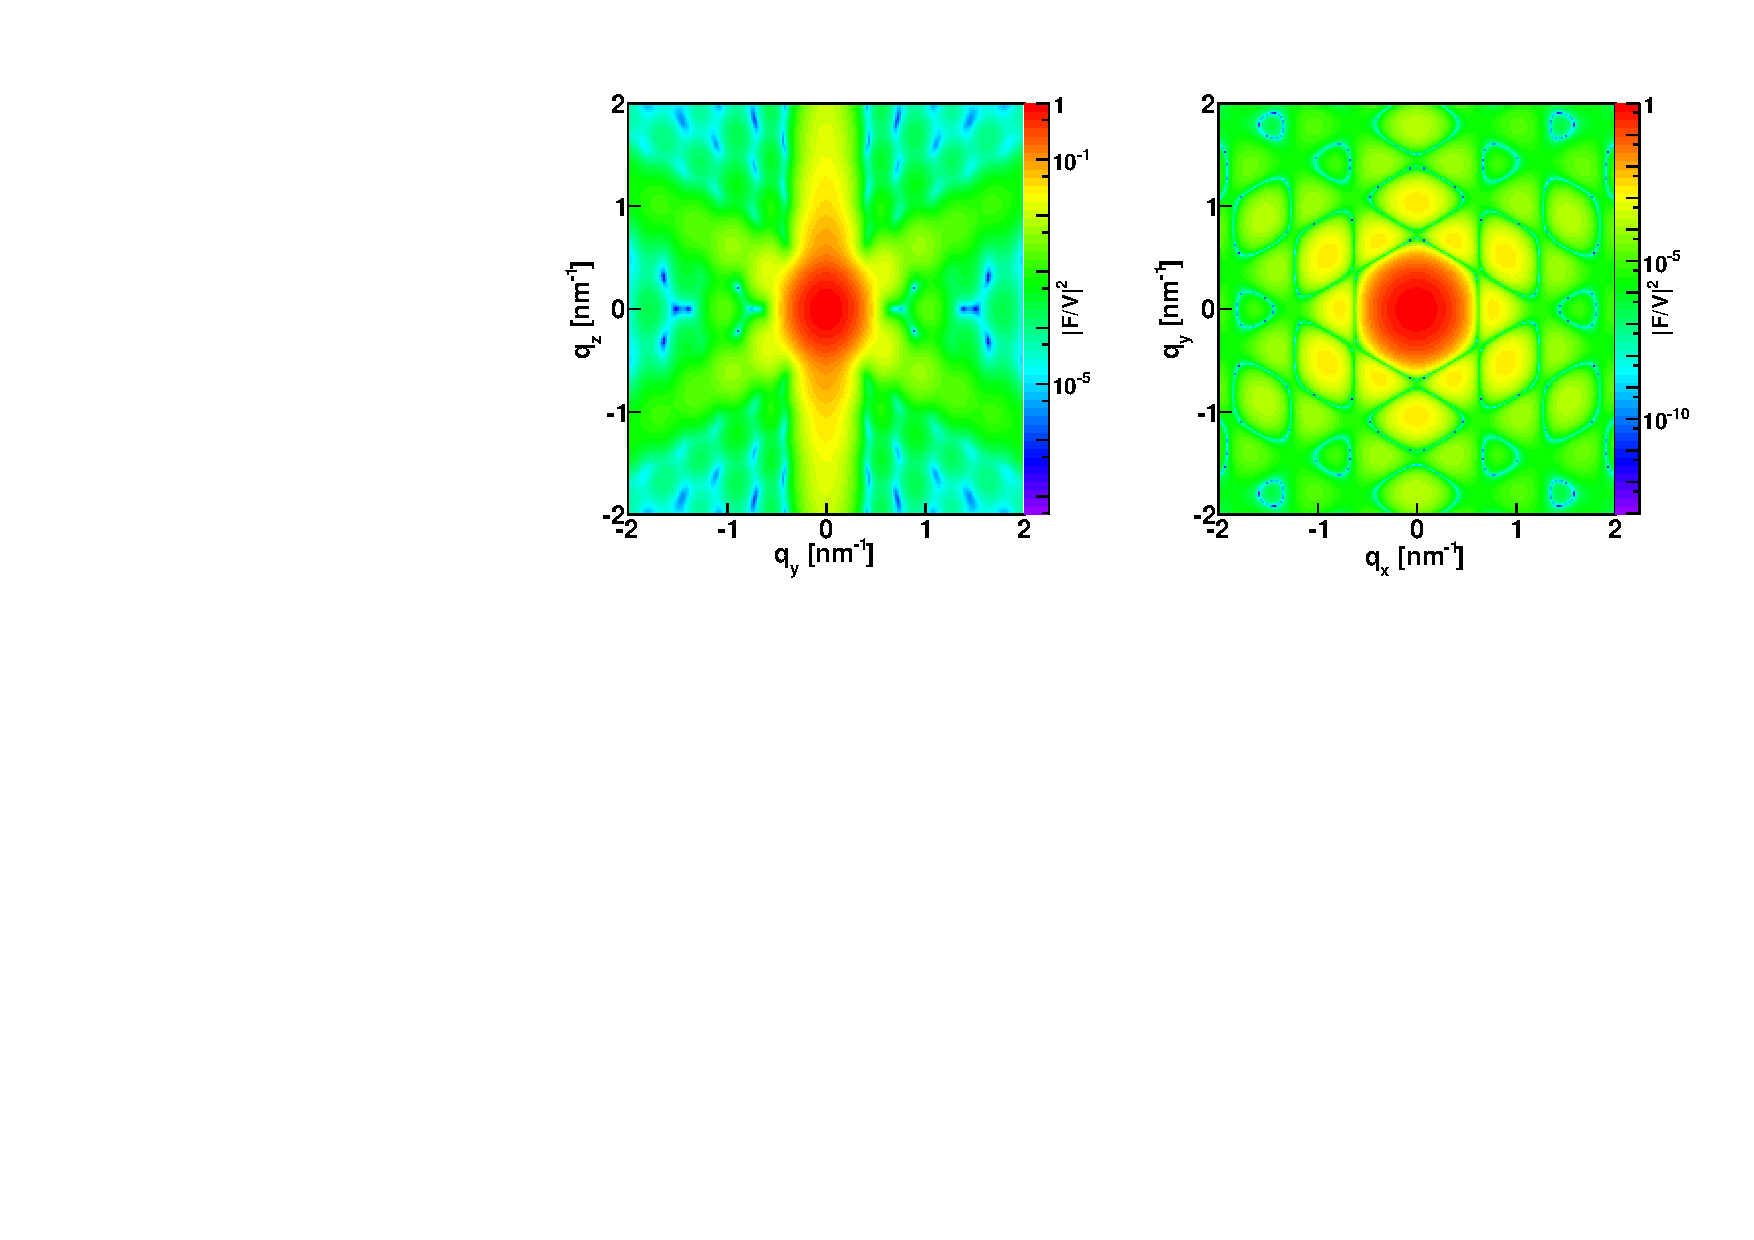
\includegraphics[width=\textwidth]{Figures/figffcone6}
\end{center}
\caption{Normalized intensity for the form factor of a Cone6 $|F|^2/V^2$, plotted against ($q_z$, $q_y$) and ($q_x$, $q_y$) and  computed with $R=10$~nm, $H=13$~nm, and $\alpha=60^{\circ}$.}
\label{fig:FFCone6Ex}
\end{figure}


\FloatBarrier

%\subsection{References}
%The convention of the base length is different
%from the one implemented in \Code{IsGISAXS}: $R =
%2/\sqrt{3}R_{\text{\Code{IsGiSAXS}}}$.

\newpage{\cleardoublepage}
%%%%%%%%%%%%%%%%%%%%%%%%%%%%%%%%%%%%
\section{Pyramid}\SecLabel{Pyramid}

\subsection{Real-space geometry}
This shape is a  truncated pyramid with a square base as shown in fig.~\ref{fig:pyramid}.

\begin{figure}[ht]
\hfill
\subfigure[Side view]{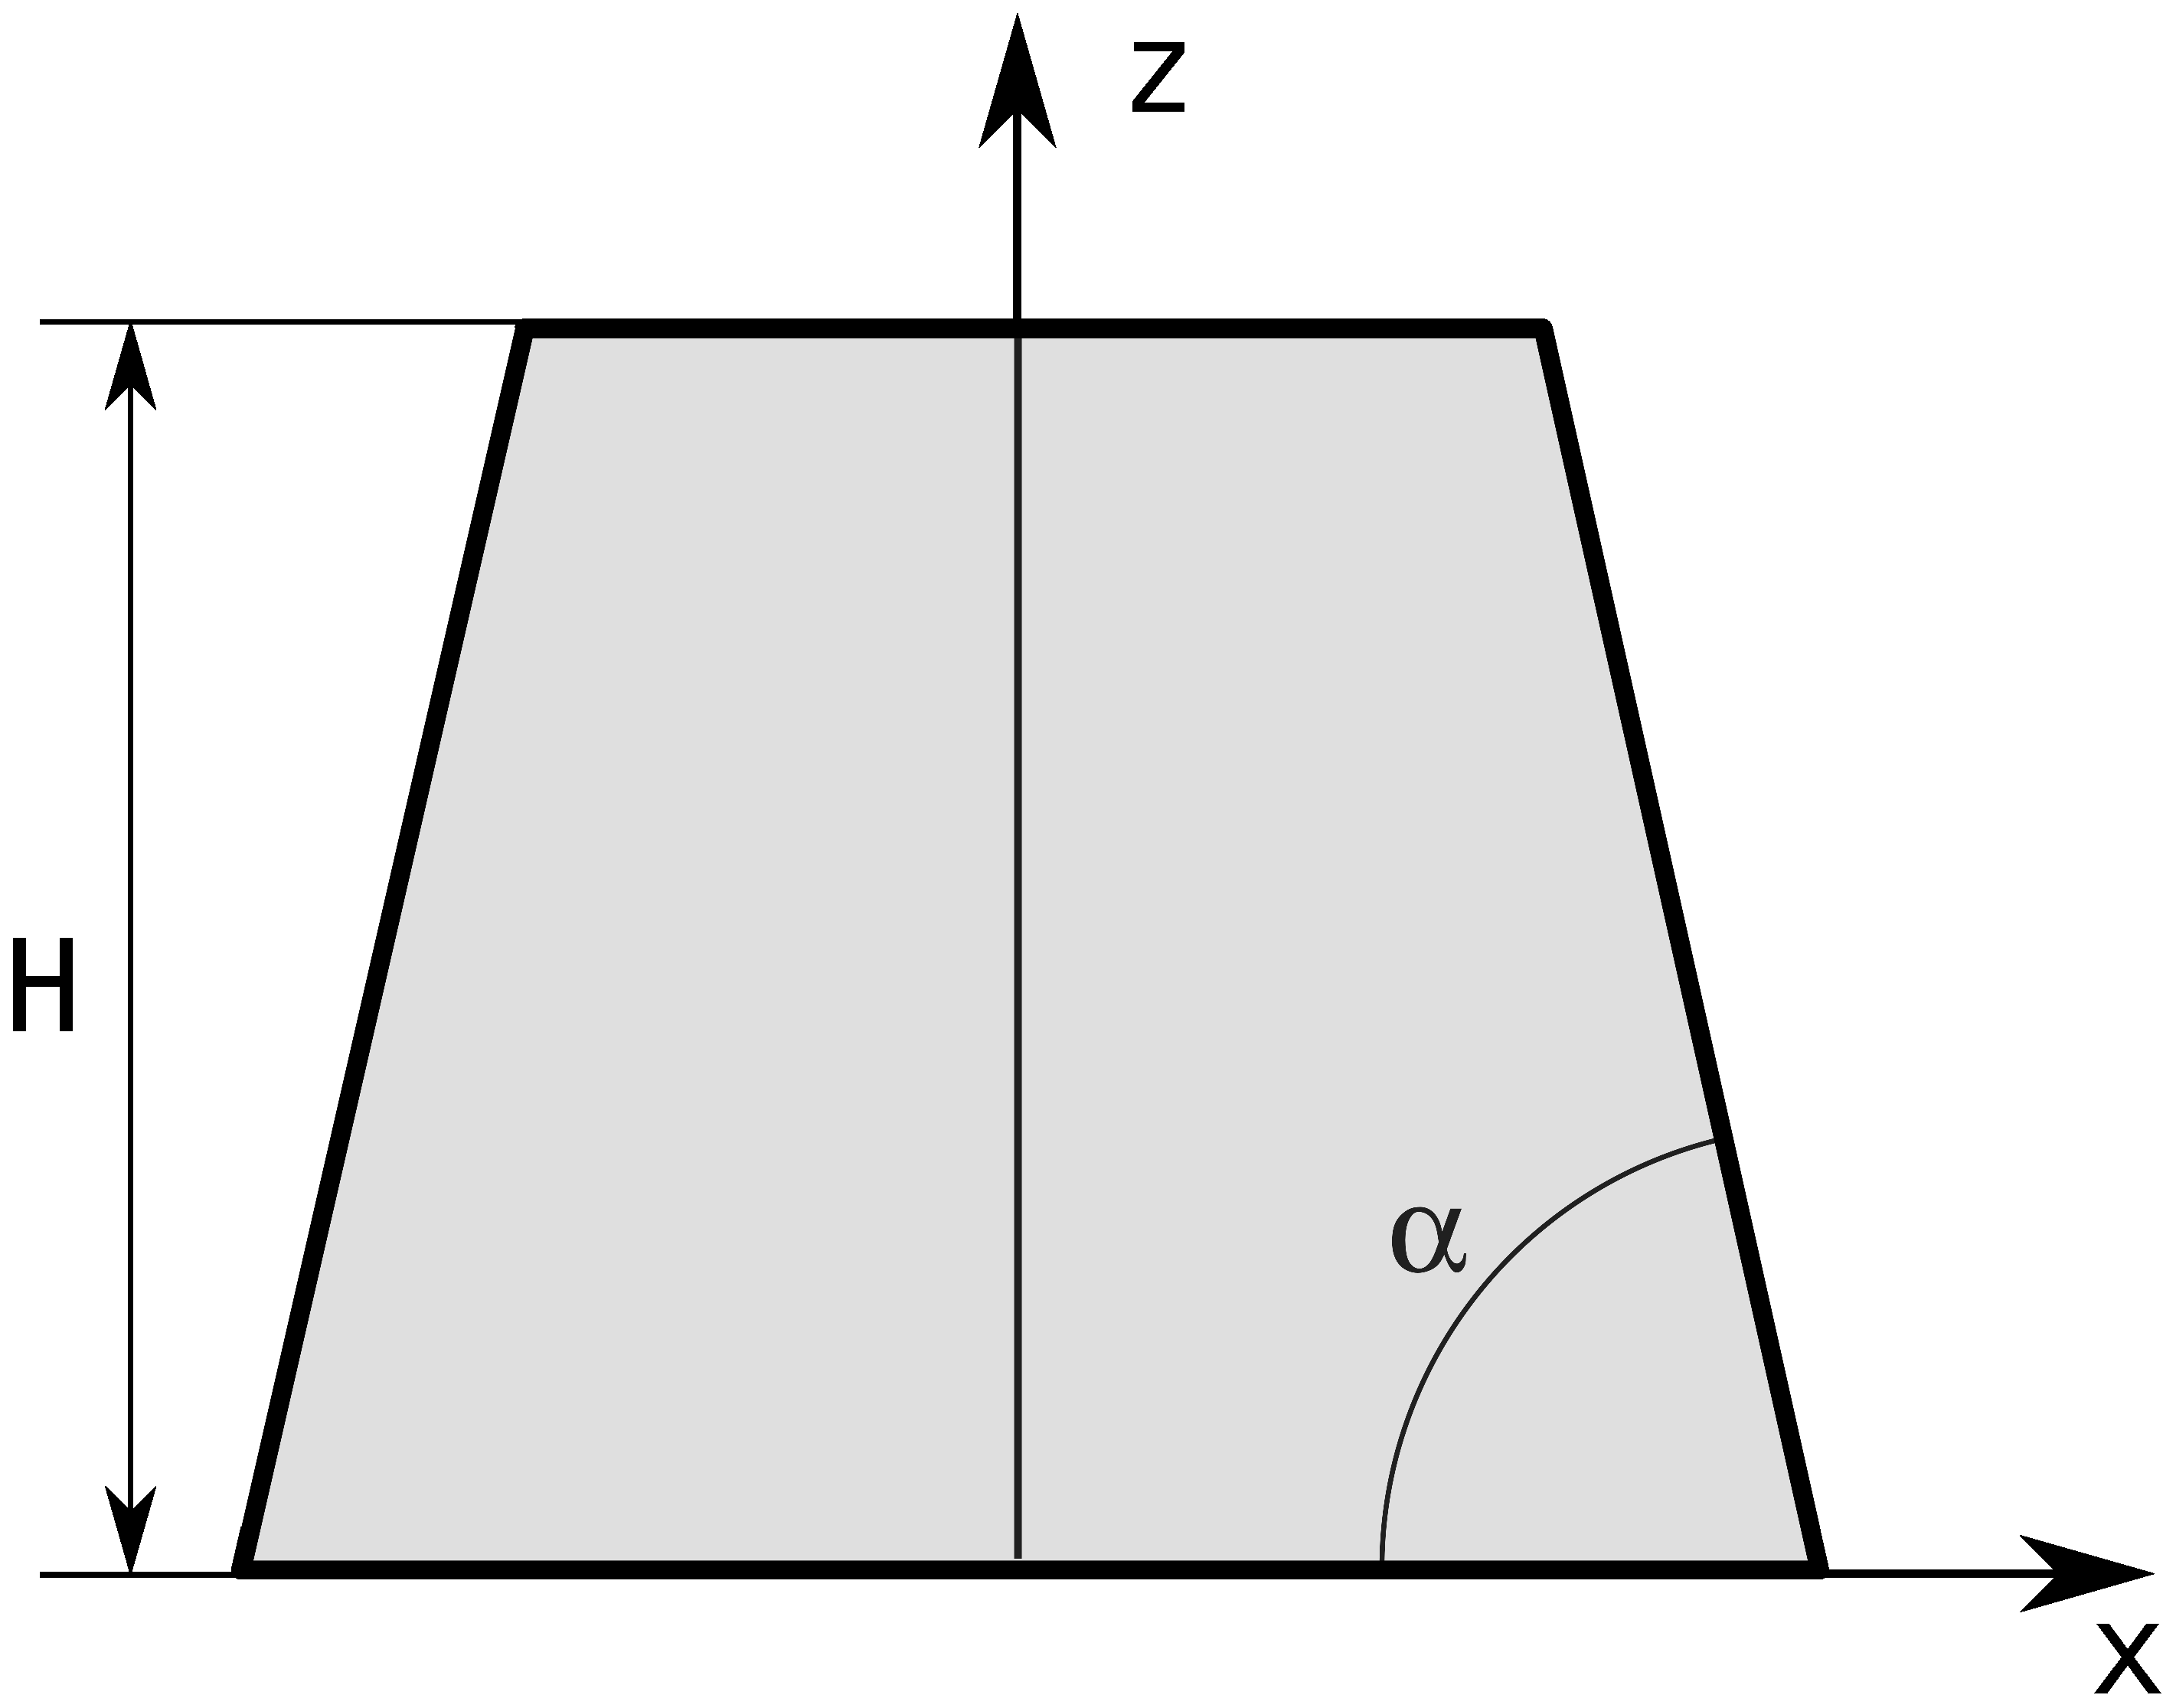
\includegraphics[width=5cm]{Figures/Pyramid2dxz}}
\hfill
\subfigure[Top view]{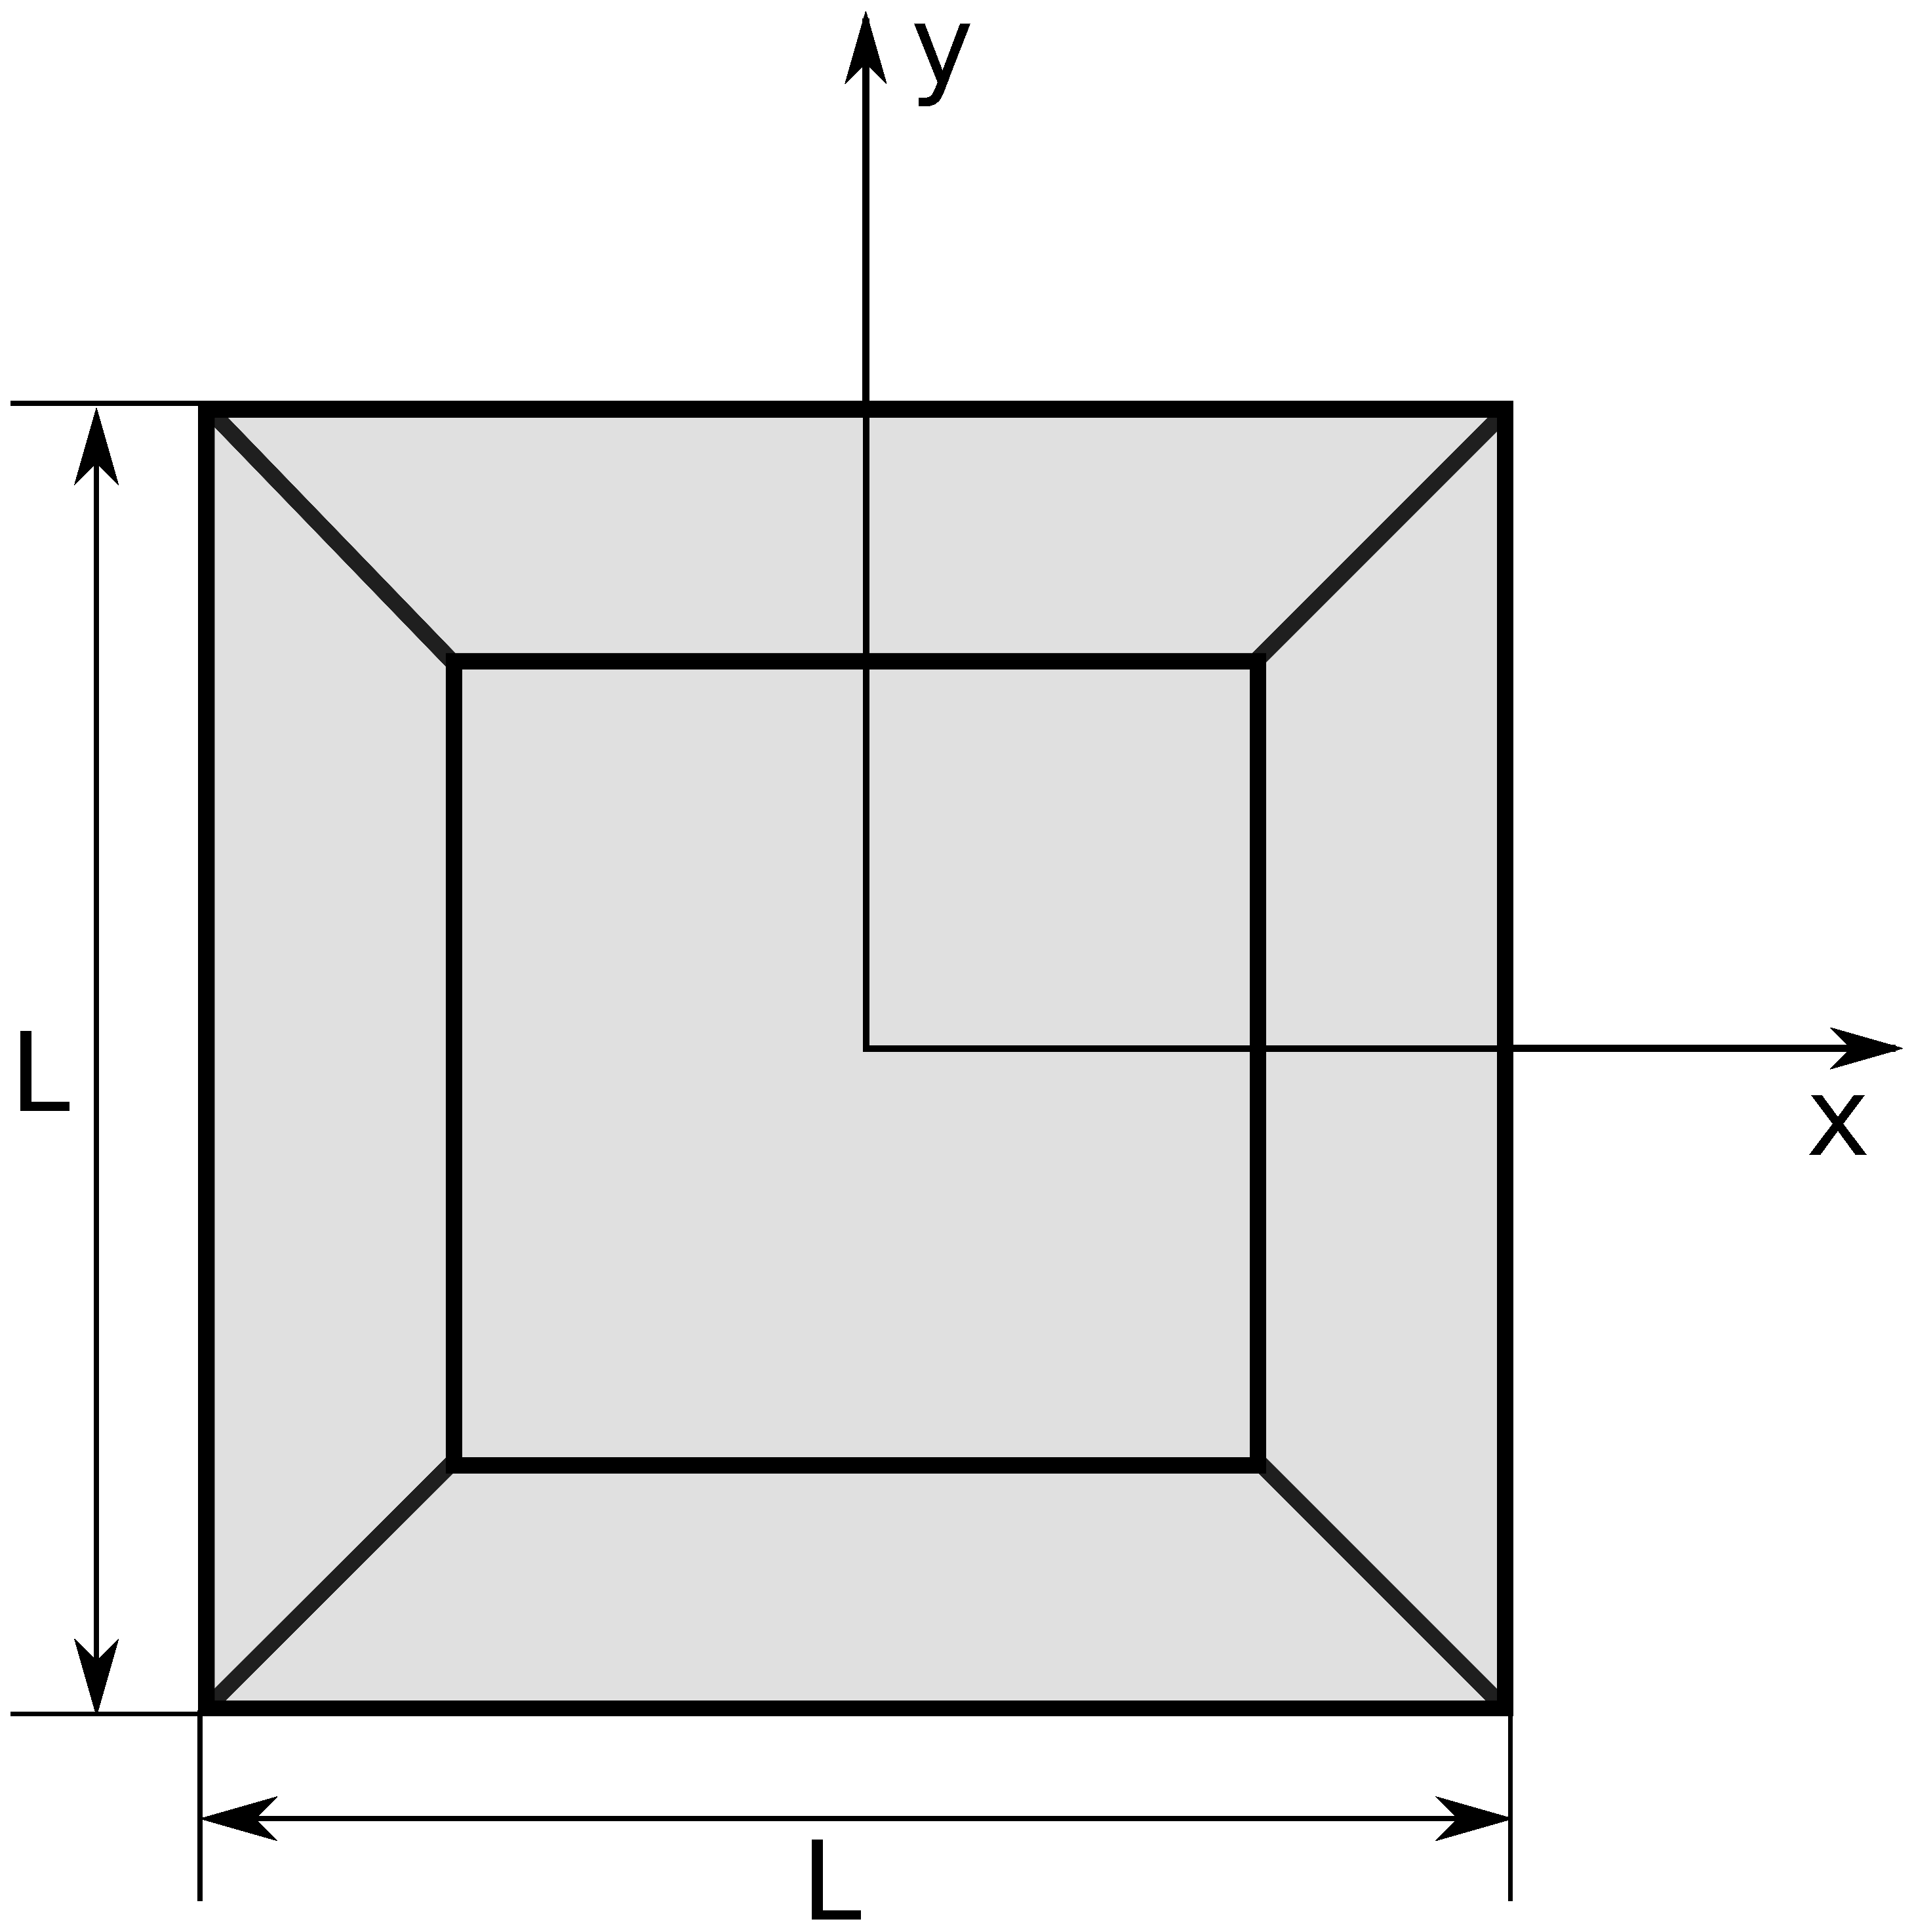
\includegraphics[width=5cm]{Figures/Pyramid2dxy}}
\hfill
\caption{Sketch of a Pyramid}
\label{fig:pyramid}
\end{figure}

\FloatBarrier

%\par
\paragraph{Parameters:}
\begin{itemize}
\item length of one side of the square base $L$,  
\item height $H$,
\item  $\alpha$ is the angle between the base and the
  side faces, taken in the middle of the base lines.
\end{itemize}

\paragraph{Restrictions on the parameters:} $\dfrac{2H}{L} < \tan(\alpha)$.

\paragraph{Properties:}
\begin{itemize}
\item  volume $V = \dfrac{1}{6} \tan(\alpha) L^3\Big[ 1
             - \big(1 - \dfrac{2H}{\tan(\alpha)L}\big)^3 \Big],$
\item particle surface seen from above $S = L^2$.
%\item gyration radius along $z$ axis $R_g = \sqrt{2}R$
\end{itemize}

\subsection{Expression of the form factor}
\begin{align*}
&F_{\rm{Pyramid}}(\mathbf{q},L, H, \alpha) =
\frac{H}{q_x q_y} \times \nonumber \\ &\left\{ K_1 \cos\left[
  (q_x-q_y)\frac{L}{2} \right] + K_2 \sin\left[ (q_x-q_y)\frac{L}{2} \right]
- K_3 \cos\left[ (q_x+q_y) \frac{L}{2} \right] - K_4 \sin\left[ (q_x+q_y)\frac{L}{2} \right]\right\},
\end{align*}
with $\sinc(x)=\sin(x)/x$,
\begin{align*}
       q_1 &=\frac{1}{2}\Big[\frac{q_x-q_y}{\tan(\alpha)} + q_z\Big],\quad       q_2 =\frac{1}{2}\Big[\frac{q_x-q_y}{\tan(\alpha)} - q_z\Big]\\
        q_3 &=\frac{1}{2}\Big[\frac{q_x+q_y}{\tan(\alpha)} + q_z\Big],\quad       q_4 =\frac{1}{2}\Big[\frac{q_x+q_y}{\tan(\alpha)} - q_z\Big]\\
        K_1 &= \sinc(q_1 H)\exp(i q_1 H)  + \sinc(q_2 H) \exp(-i q_2 H)\\
        K_2 &= -i \sinc(q_1 H) \exp(i q_1 H) +i \sinc(q_2 H) \exp(-i q_2 H)\\
        K_3 &= \sinc(q_3 H) \exp(i q_3 H)    + \sinc(q_4 H) \exp(-i q_4 H)\\
        K_4 &= -i \sinc(q_3 H) \exp(i q_3 H) + i \sinc(q_4 H) \exp(-i q_4 H) 
   \end{align*}

\paragraph{Syntax:}  \Code{FormFactorPyramid(length, height, alpha)}

\subsection{Examples}
Figure~\ref{fig:FFPyramidEx} shows the normalized intensity
$|F|^2/V^2$, computed with $L=18$~nm, $H=13$~nm and
$\alpha=60^{\circ}$.

\begin{figure}[h]
\begin{center}
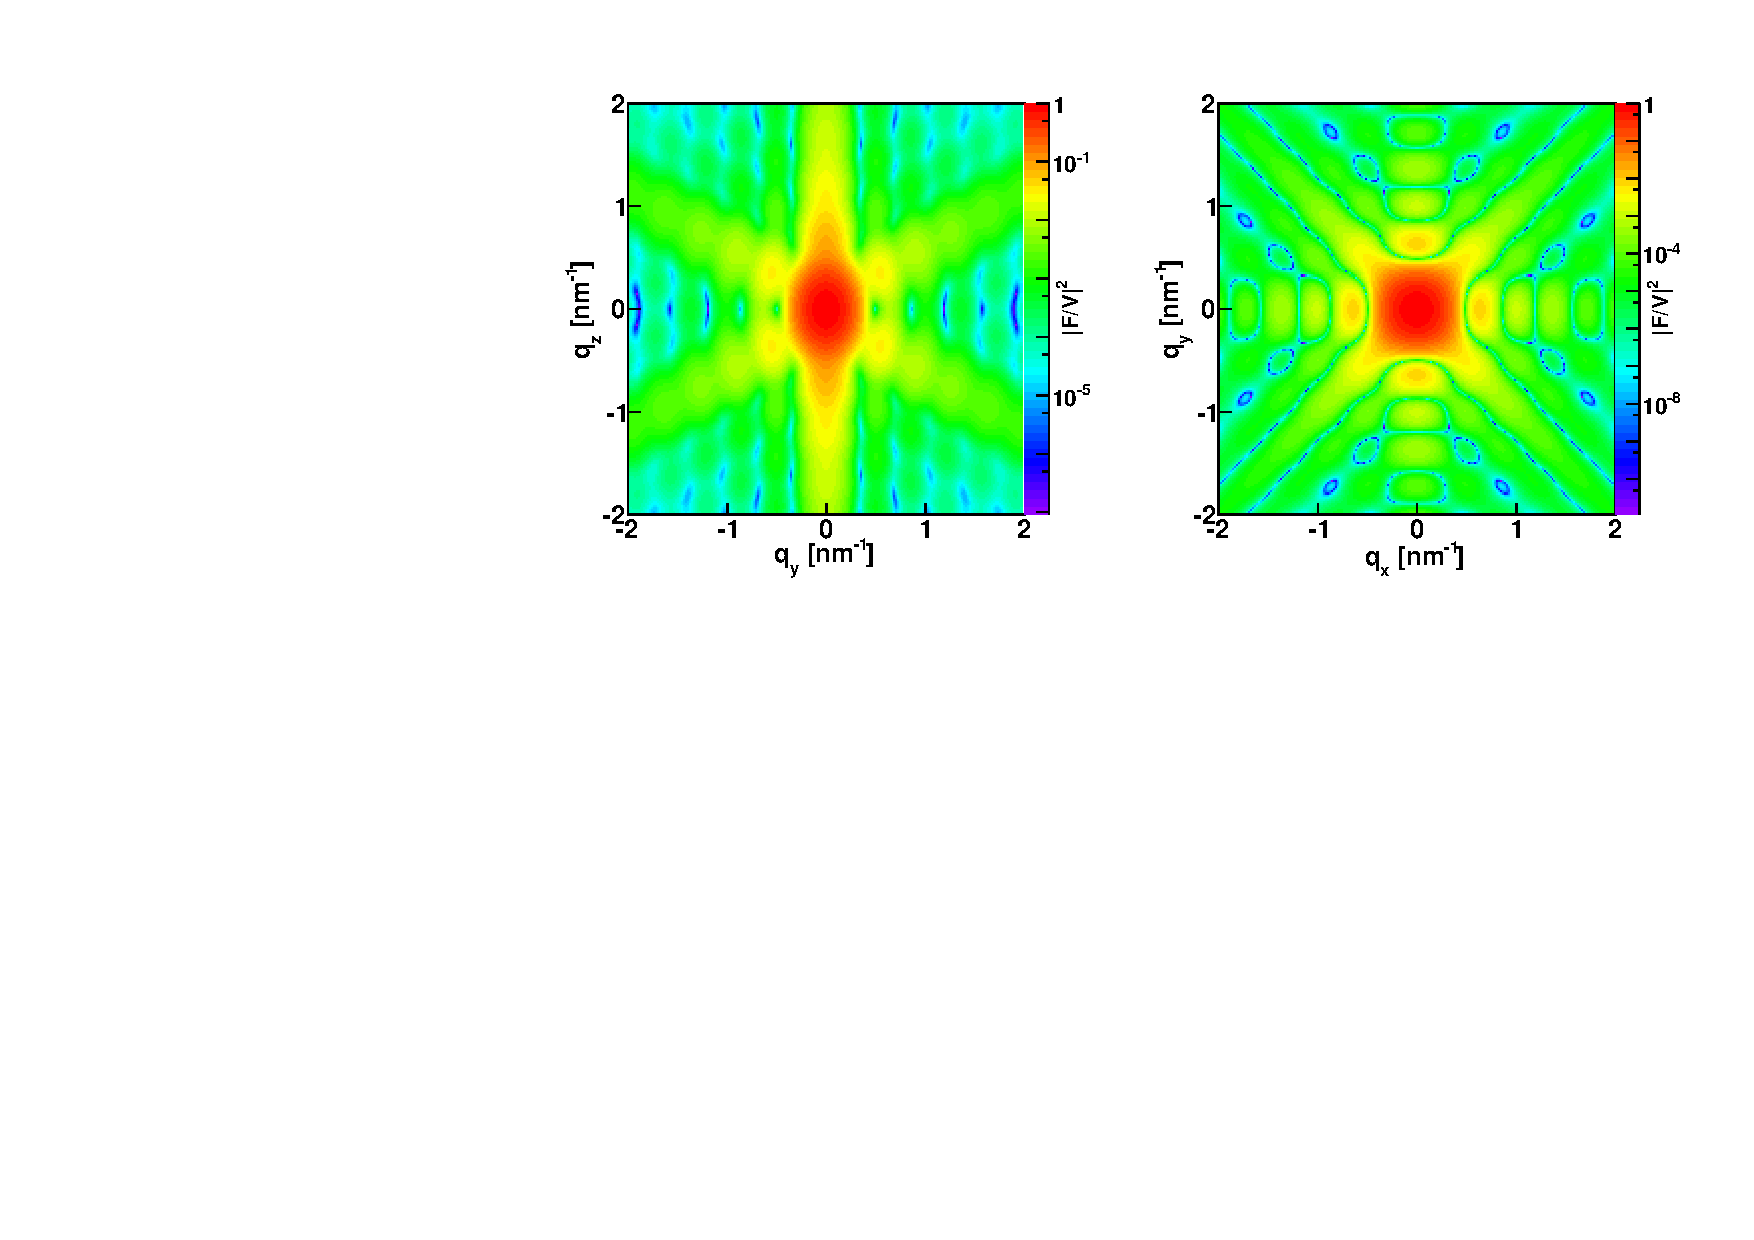
\includegraphics[width=\textwidth]{Figures/figffpyramid}
\end{center}
\caption{Normalized intensity for the form factor of a
  pyramid $|F|^2/V^2$, plotted against ($q_z$, $q_y$) and  
  ($q_x$, $q_y$) and computed with $L=18$~nm and $H=13$~nm, and $\alpha=60^{\circ}$.}
\label{fig:FFPyramidEx}
\end{figure}

\FloatBarrier

%\subsection{References}
%The output of equation~(\ref{eq:ffpyramid}) agrees with the \lq\lq
%pyramid\rq\rq ~form factor of \IsGISAXS~\cite{Laz02}.

%In \BornAgain\, the base of the pyramid is characterized by the full
%length of one of its side and not by half this value: $L=2R_{\rm{\Code{IsGISXAXS}}}$. 
%Pyramid: problem with signs of K2 and K4

\newpage{\cleardoublepage}
%%%%%%%%%%%%%%%%%%%%%%%%%%%%%%%%%%%%
\section{Anisotropic pyramid} \SecLabel{AnisoPyramid} 

\subsection{Real-space geometry}
This shape is a truncated right pyramid with a rectangular base as
shown in fig.~\ref{fig:anisopyramid}.

\begin{figure}[ht]
\hfill
\subfigure[Side view]{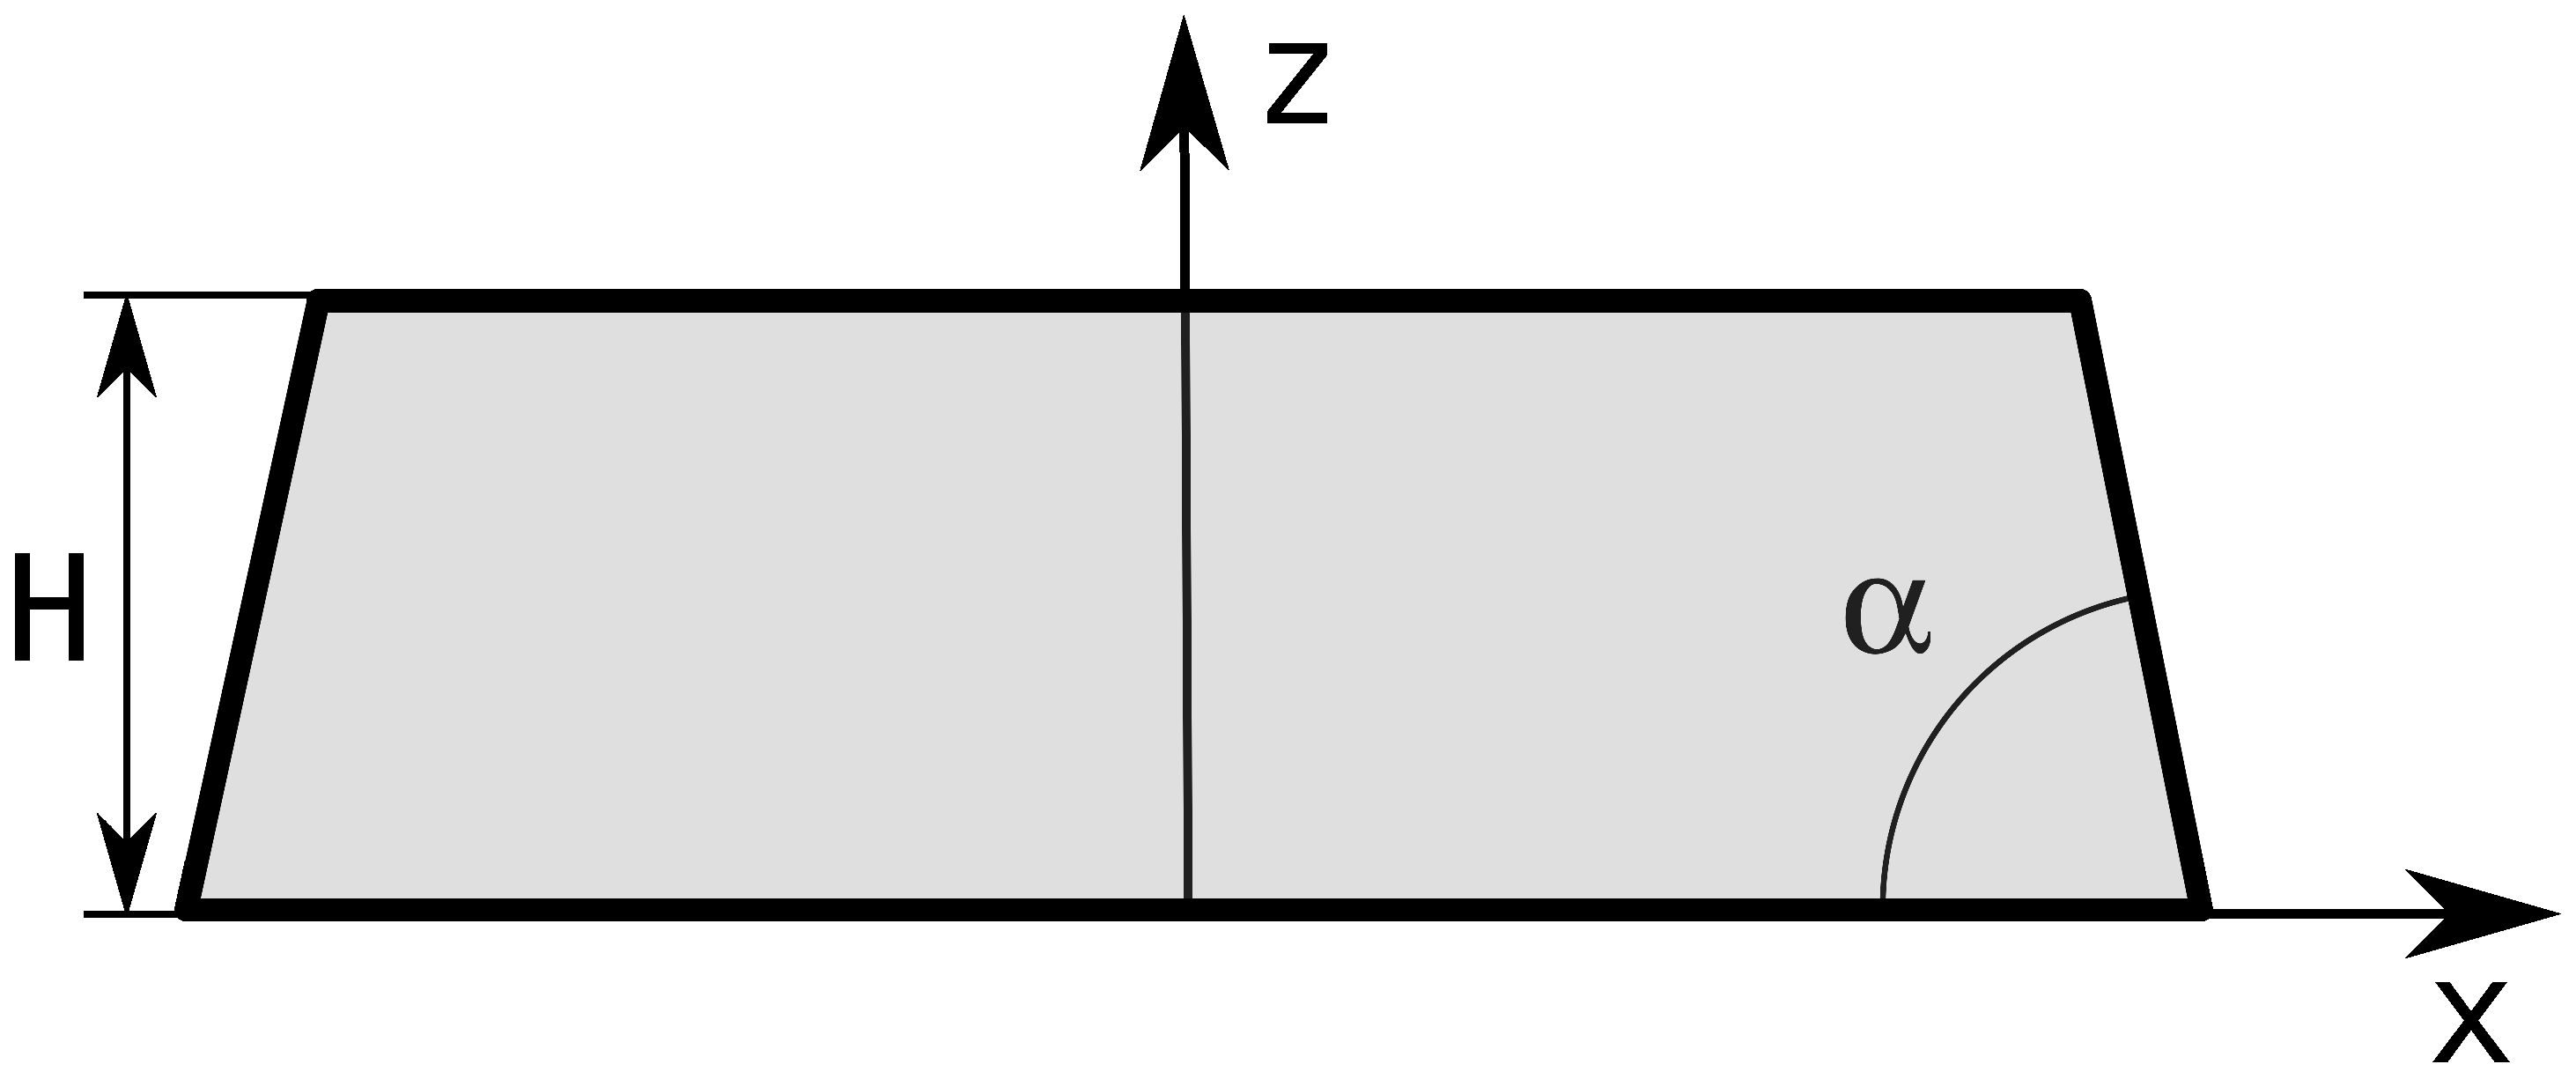
\includegraphics[width=5cm]{Figures/AnisoPyramid2dxz.eps}}
\hfill
\subfigure[Top view]{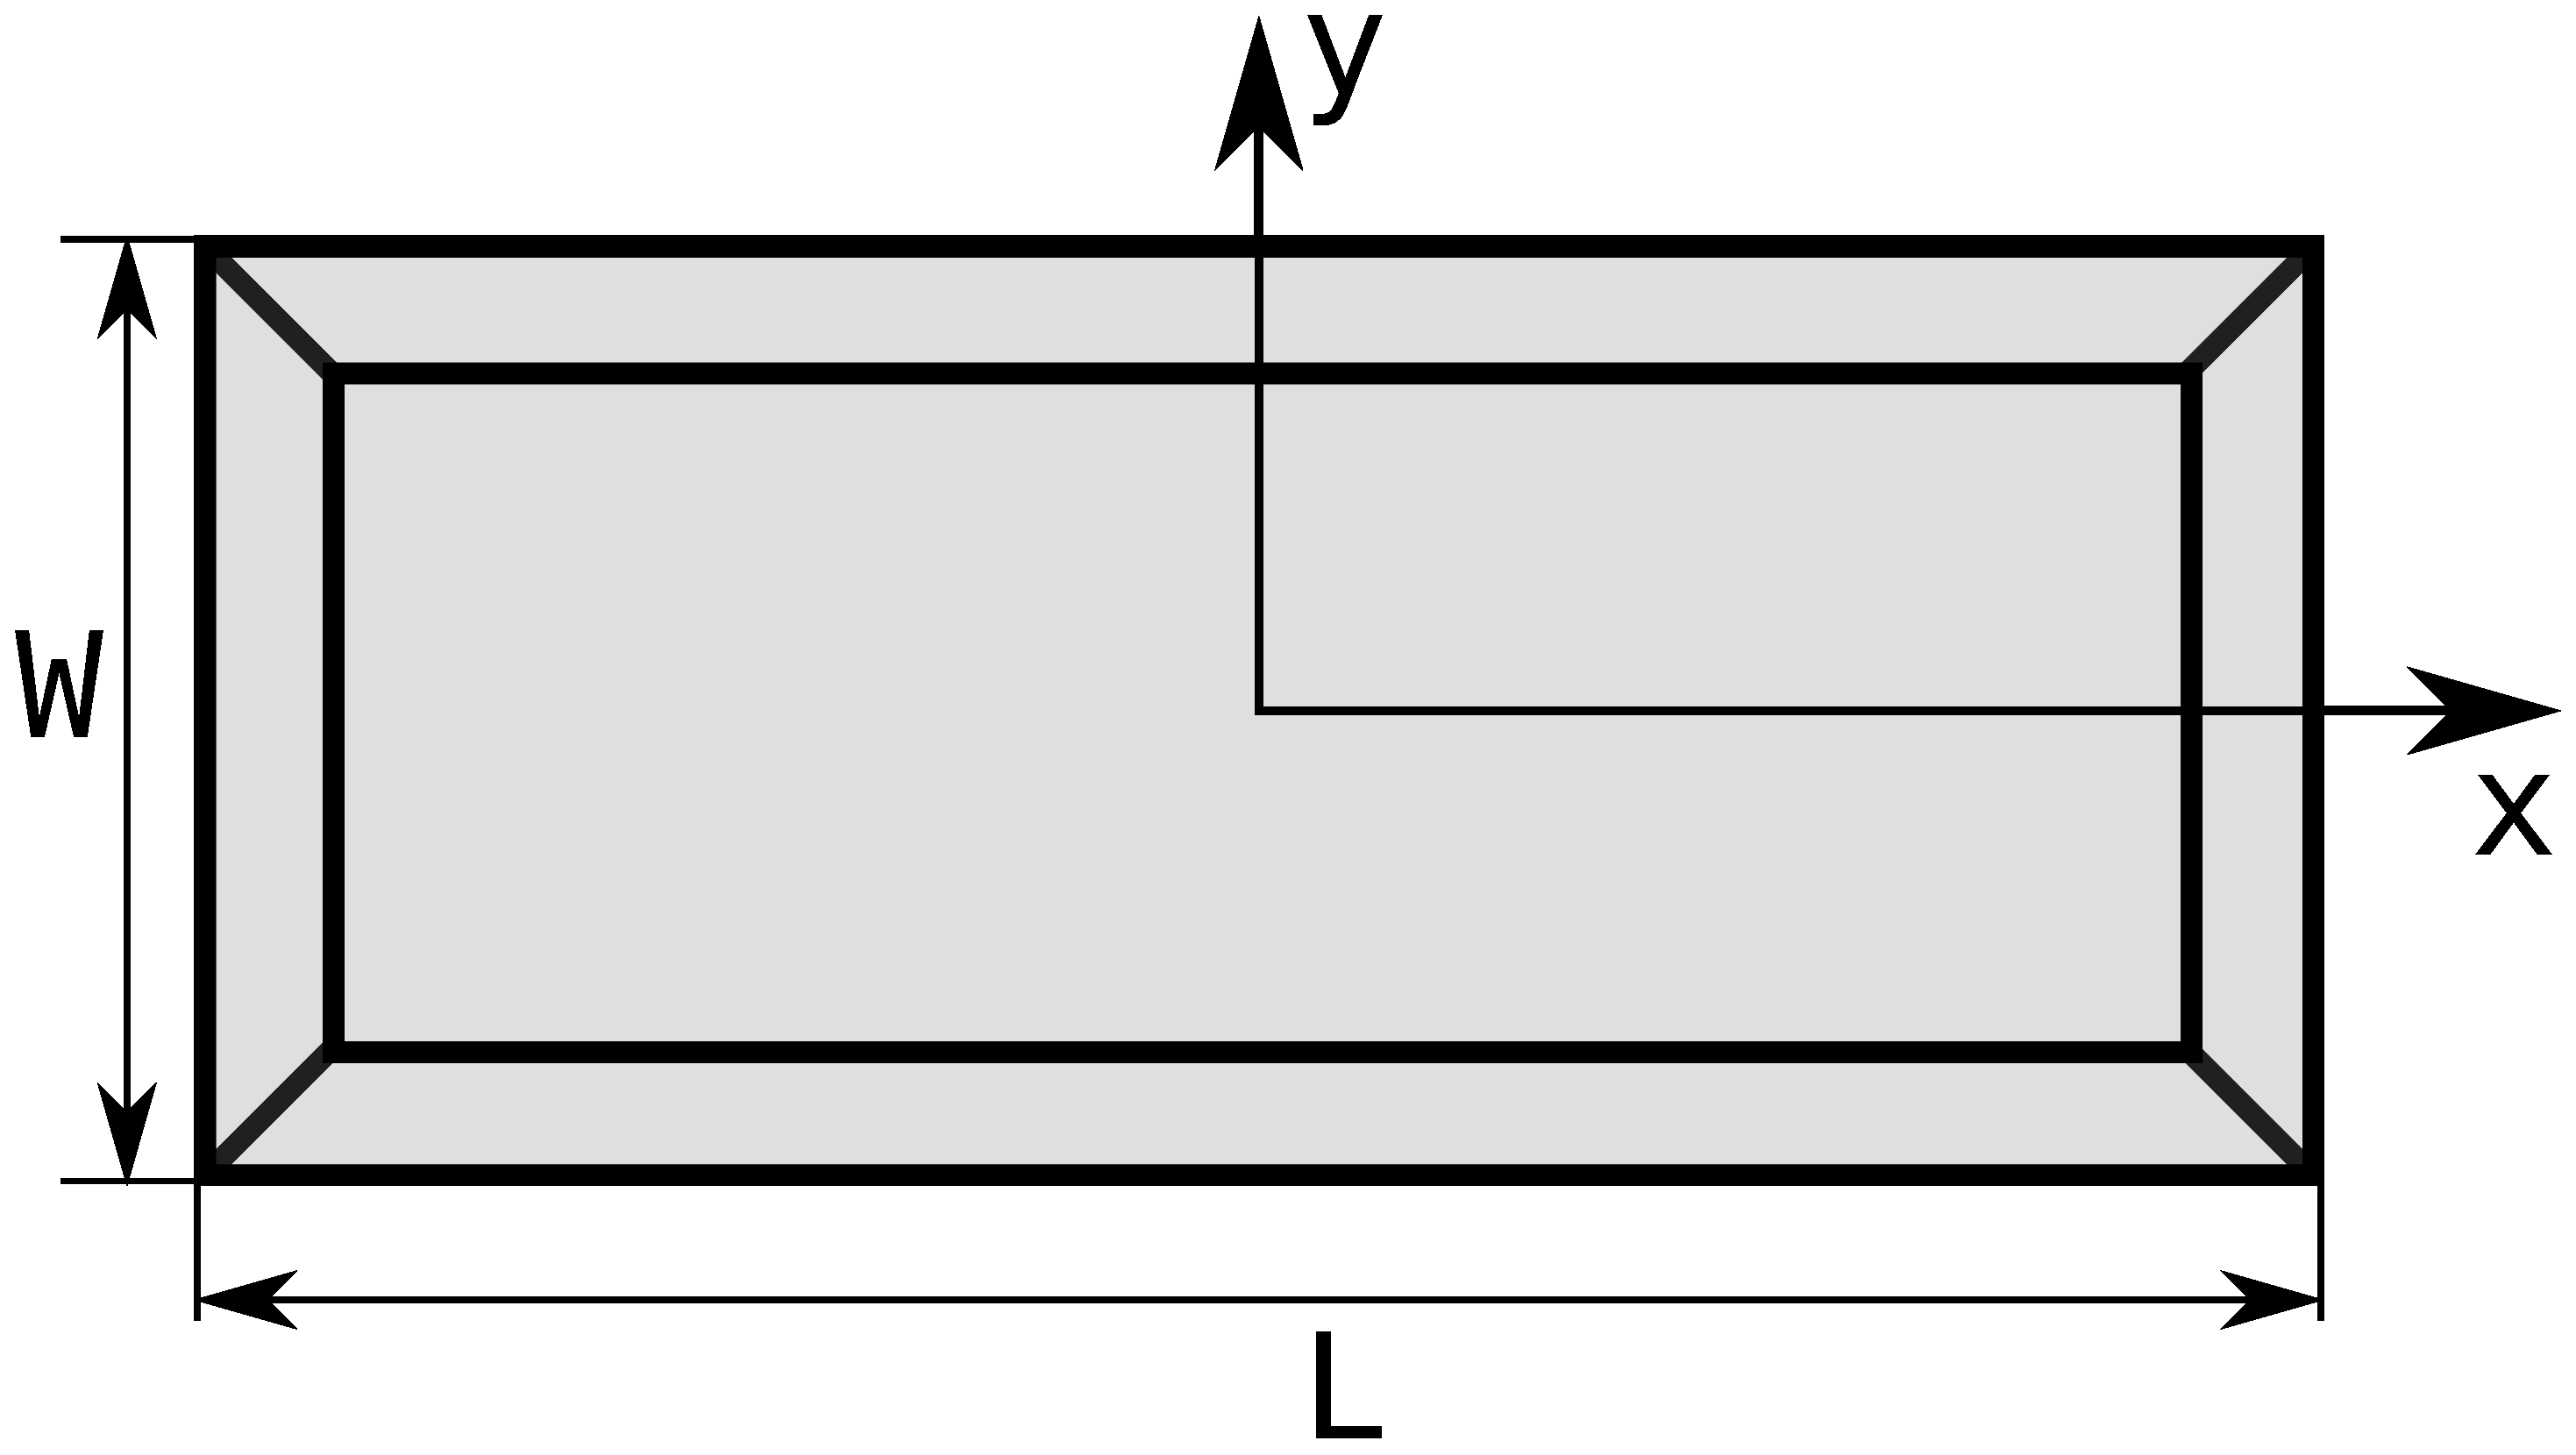
\includegraphics[width=5cm]{Figures/AnisoPyramid2dxy.eps}}
\hfill
\caption{Sketch of an Anisotropic Pyramid. }
\label{fig:anisopyramid}
\end{figure}

\FloatBarrier

\paragraph{Parameters:}
\begin{itemize}
\item full length of the base $L$,
\item full width of the base $W$,
\item height $H$,
\item $\alpha$ is the angle between the base and the
  side faces, taken in the middle of the base lines.
\end{itemize}

\paragraph{Restrictions on the parameters:} $\dfrac{2H}{L}< \tan(\alpha)$ and $\dfrac{2H}{W}< \tan(\alpha)$.

\paragraph{Properties:}
\begin{itemize}
\item volume $V= H \Big[LW - \dfrac{(L + W)H}{\tan(\alpha)}
   + \dfrac{4}{3} \dfrac{H^2}{\tan^2(\alpha)}\Big]$,
\item particle surface seen from above $S = LW$.
%\item radius of gyration
\end{itemize}

\subsection{Expression of the form factor}
\begin{align*}
&F_{\rm{AnisoPyramid}}(\mathbf{q}, L, W, H, \alpha)=
\frac{H}{q_xq_y} \times \\
&\Big\{
K_1\cos\Big(q_x \frac{L}{2} -q_y \frac{W}{2}\Big)+  K_2 \sin \Big (q_x
\frac{L}{2}- q_y \frac{W}{2}\Big) - K_3 \cos \Big (q_x \frac{L}{2} +q_y \frac{W}{2}\Big)-
K_4 \sin \Big (q_x \frac{L}{2} + q_y \frac{W}{2}\Big)
\Big\},
\end{align*}
with $\sinc(x)=\sin(x)/x$,
\begin{align*}
K_1 &= \exp(-i q_2 H) \sinc(q_2 H) + \exp(iq_1 H) \sinc(q_1 H) \\
K_2 &= i \exp(-iq_2 H) \sinc(q_2 H) -i \exp(iq_1 H) \sinc(q_1 H) \\
K_3 &= \exp(-iq_4 H) \sinc(q_4 H) + \exp(iq_3 H) \sinc(q_3 H) \\
K_4 &= i \exp(i q_4 H) \sinc(q_4 H) -i \exp(iq_3 H) \sinc(q_3 H)\\
q_1 &= \frac{1}{2}\left[\frac{q_x -q_y}{\tan \alpha} +q_z \right],\quad q_2 = \frac{1}{2}\left[\frac{q_x -q_y}{\tan \alpha} -q_z \right]\\
q_3 &= \frac{1}{2}\left[\frac{q_x +q_y}{\tan \alpha} +q_z \right] , \quad q_4 = \frac{1}{2}\left[\frac{q_x +q_y}{\tan \alpha} -q_z \right]
\end{align*}

\paragraph{Syntax:} \Code{FormFactorAnisoPyramid(length, width, height, alpha)}

\subsection{Examples}
Figure~\ref{fig:FFAnisoPyramidEx} shows the normalized intensity
$|F|^2/V^2$, computed with $L=20$~nm, $W=16$~nm, $H=13$~nm, and
$\alpha=60^{\circ}$.

\begin{figure}[h]
\begin{center}
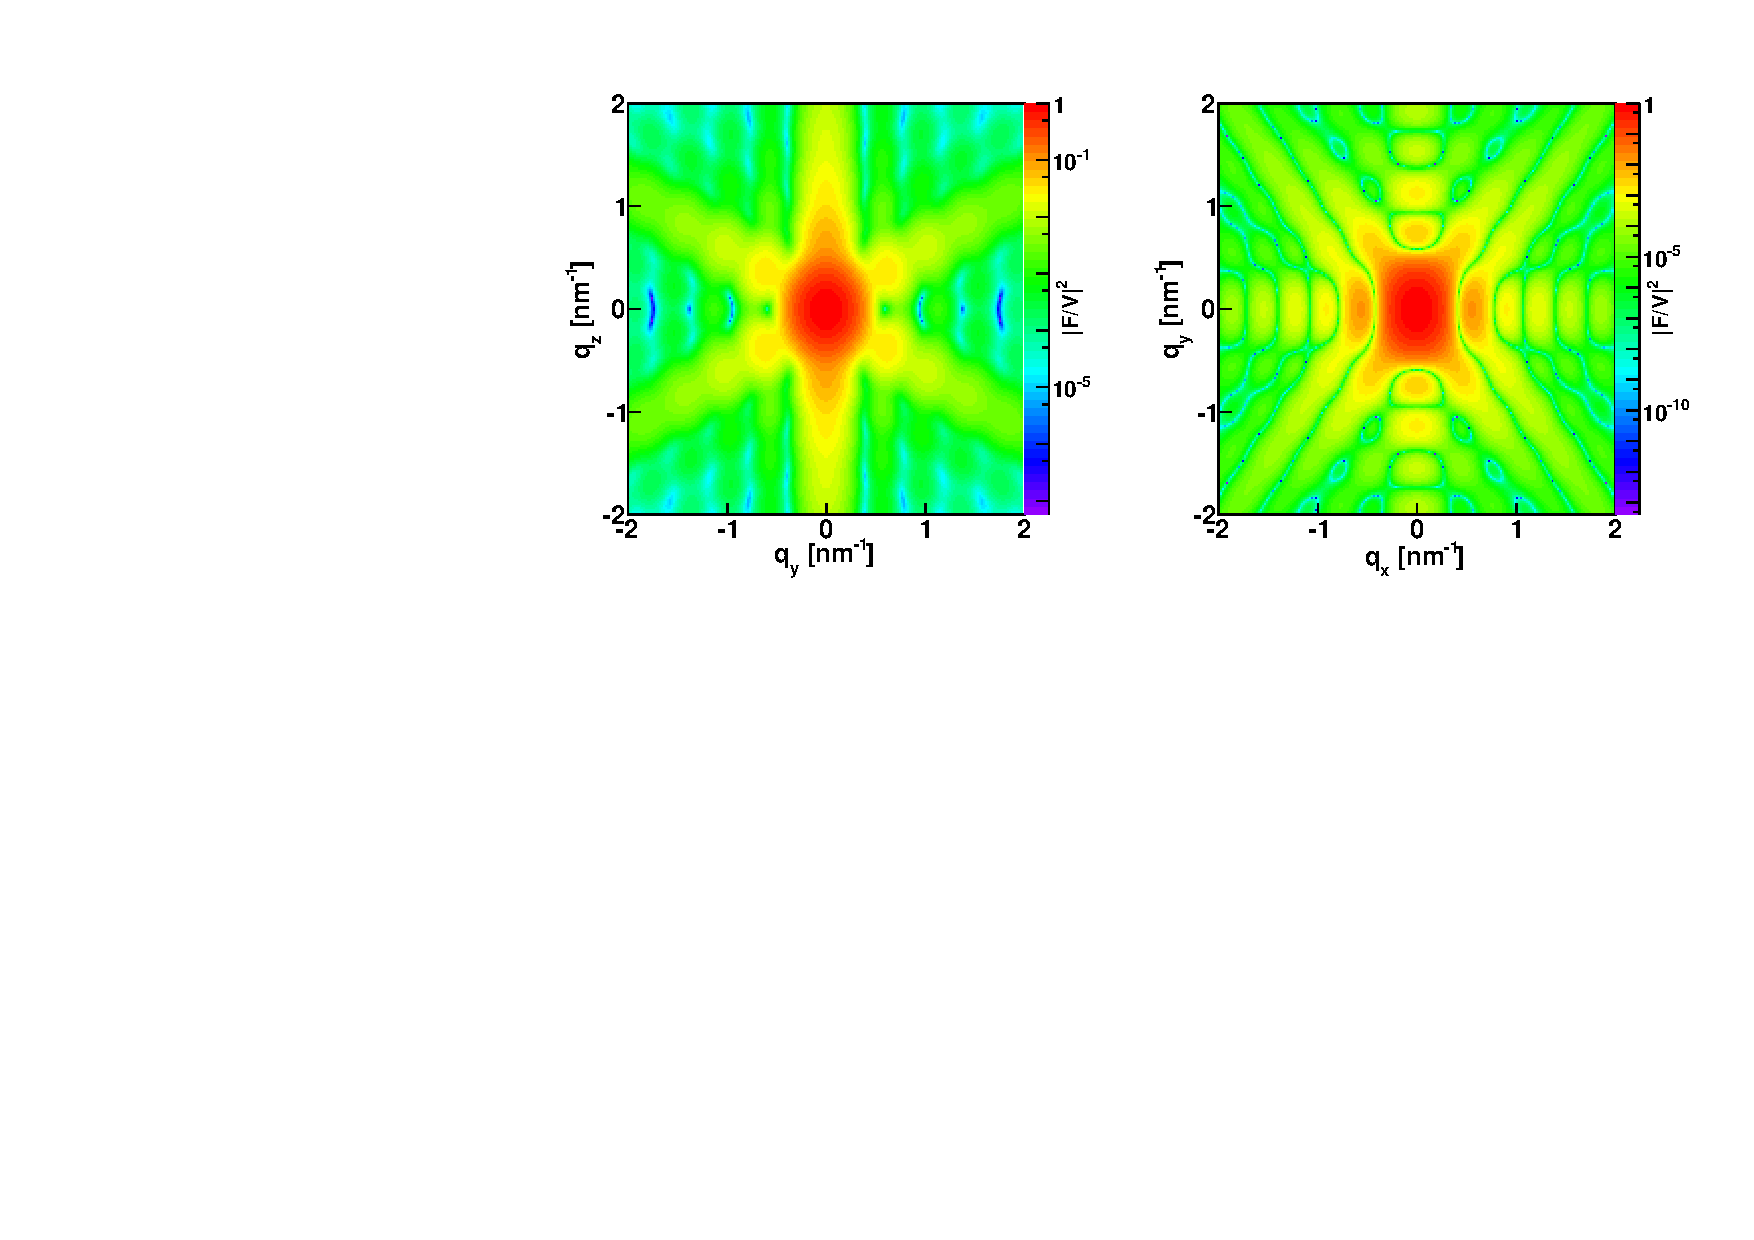
\includegraphics[width=\textwidth]{Figures/figffanisopyramid}
\end{center}
\caption{Normalized intensity for the form factor of an anisotropic
  pyramid $|F|^2/V^2$, plotted against ($q_z$, $q_y$) and  ($q_x$, $q_y$) and computed with $L=20$~nm, $W=16$~nm, $H=13$~nm,
  and $\alpha=60^{\circ}$.}
\label{fig:FFAnisoPyramidEx}
\end{figure}

\FloatBarrier

%\subsection{References}
%Like in \Code{IsGISAXS}, the base angle $\alpha$ is the same for both unequal
%side. This means that a full anisotropic pyramid is not a limit case. \\
%But \BornAgain\ uses a different convention of the parameters relative
%to the base. We input the full length and width instead of half values.
%Condition on the parameters: 
%Should not it be: H/R < tan(alpha) and  H/W < tan(alpha) instead of H/R < tan(alpha) and  W/R < tan(alpha) where H is the height and R, W the side-lengths of the rectangular base?

\newpage{\cleardoublepage}
%%%%%%%%%%%%%%%%%%%%%%%%%%%%%%%%%%%%
\section{Cuboctahedron} \SecLabel{Cuboctahedron} 

\subsection{Real-space geometry}
It is a combination of two pyramids with square bases, as shown in fig.~\ref{fig:cuboctahedron}: the bottom one
is upside down with an height $H$ and the top one has the opposite
orientation (the standard one) and an height $r_H H$.

\begin{figure}[ht]
\hfill
\subfigure[Side view]{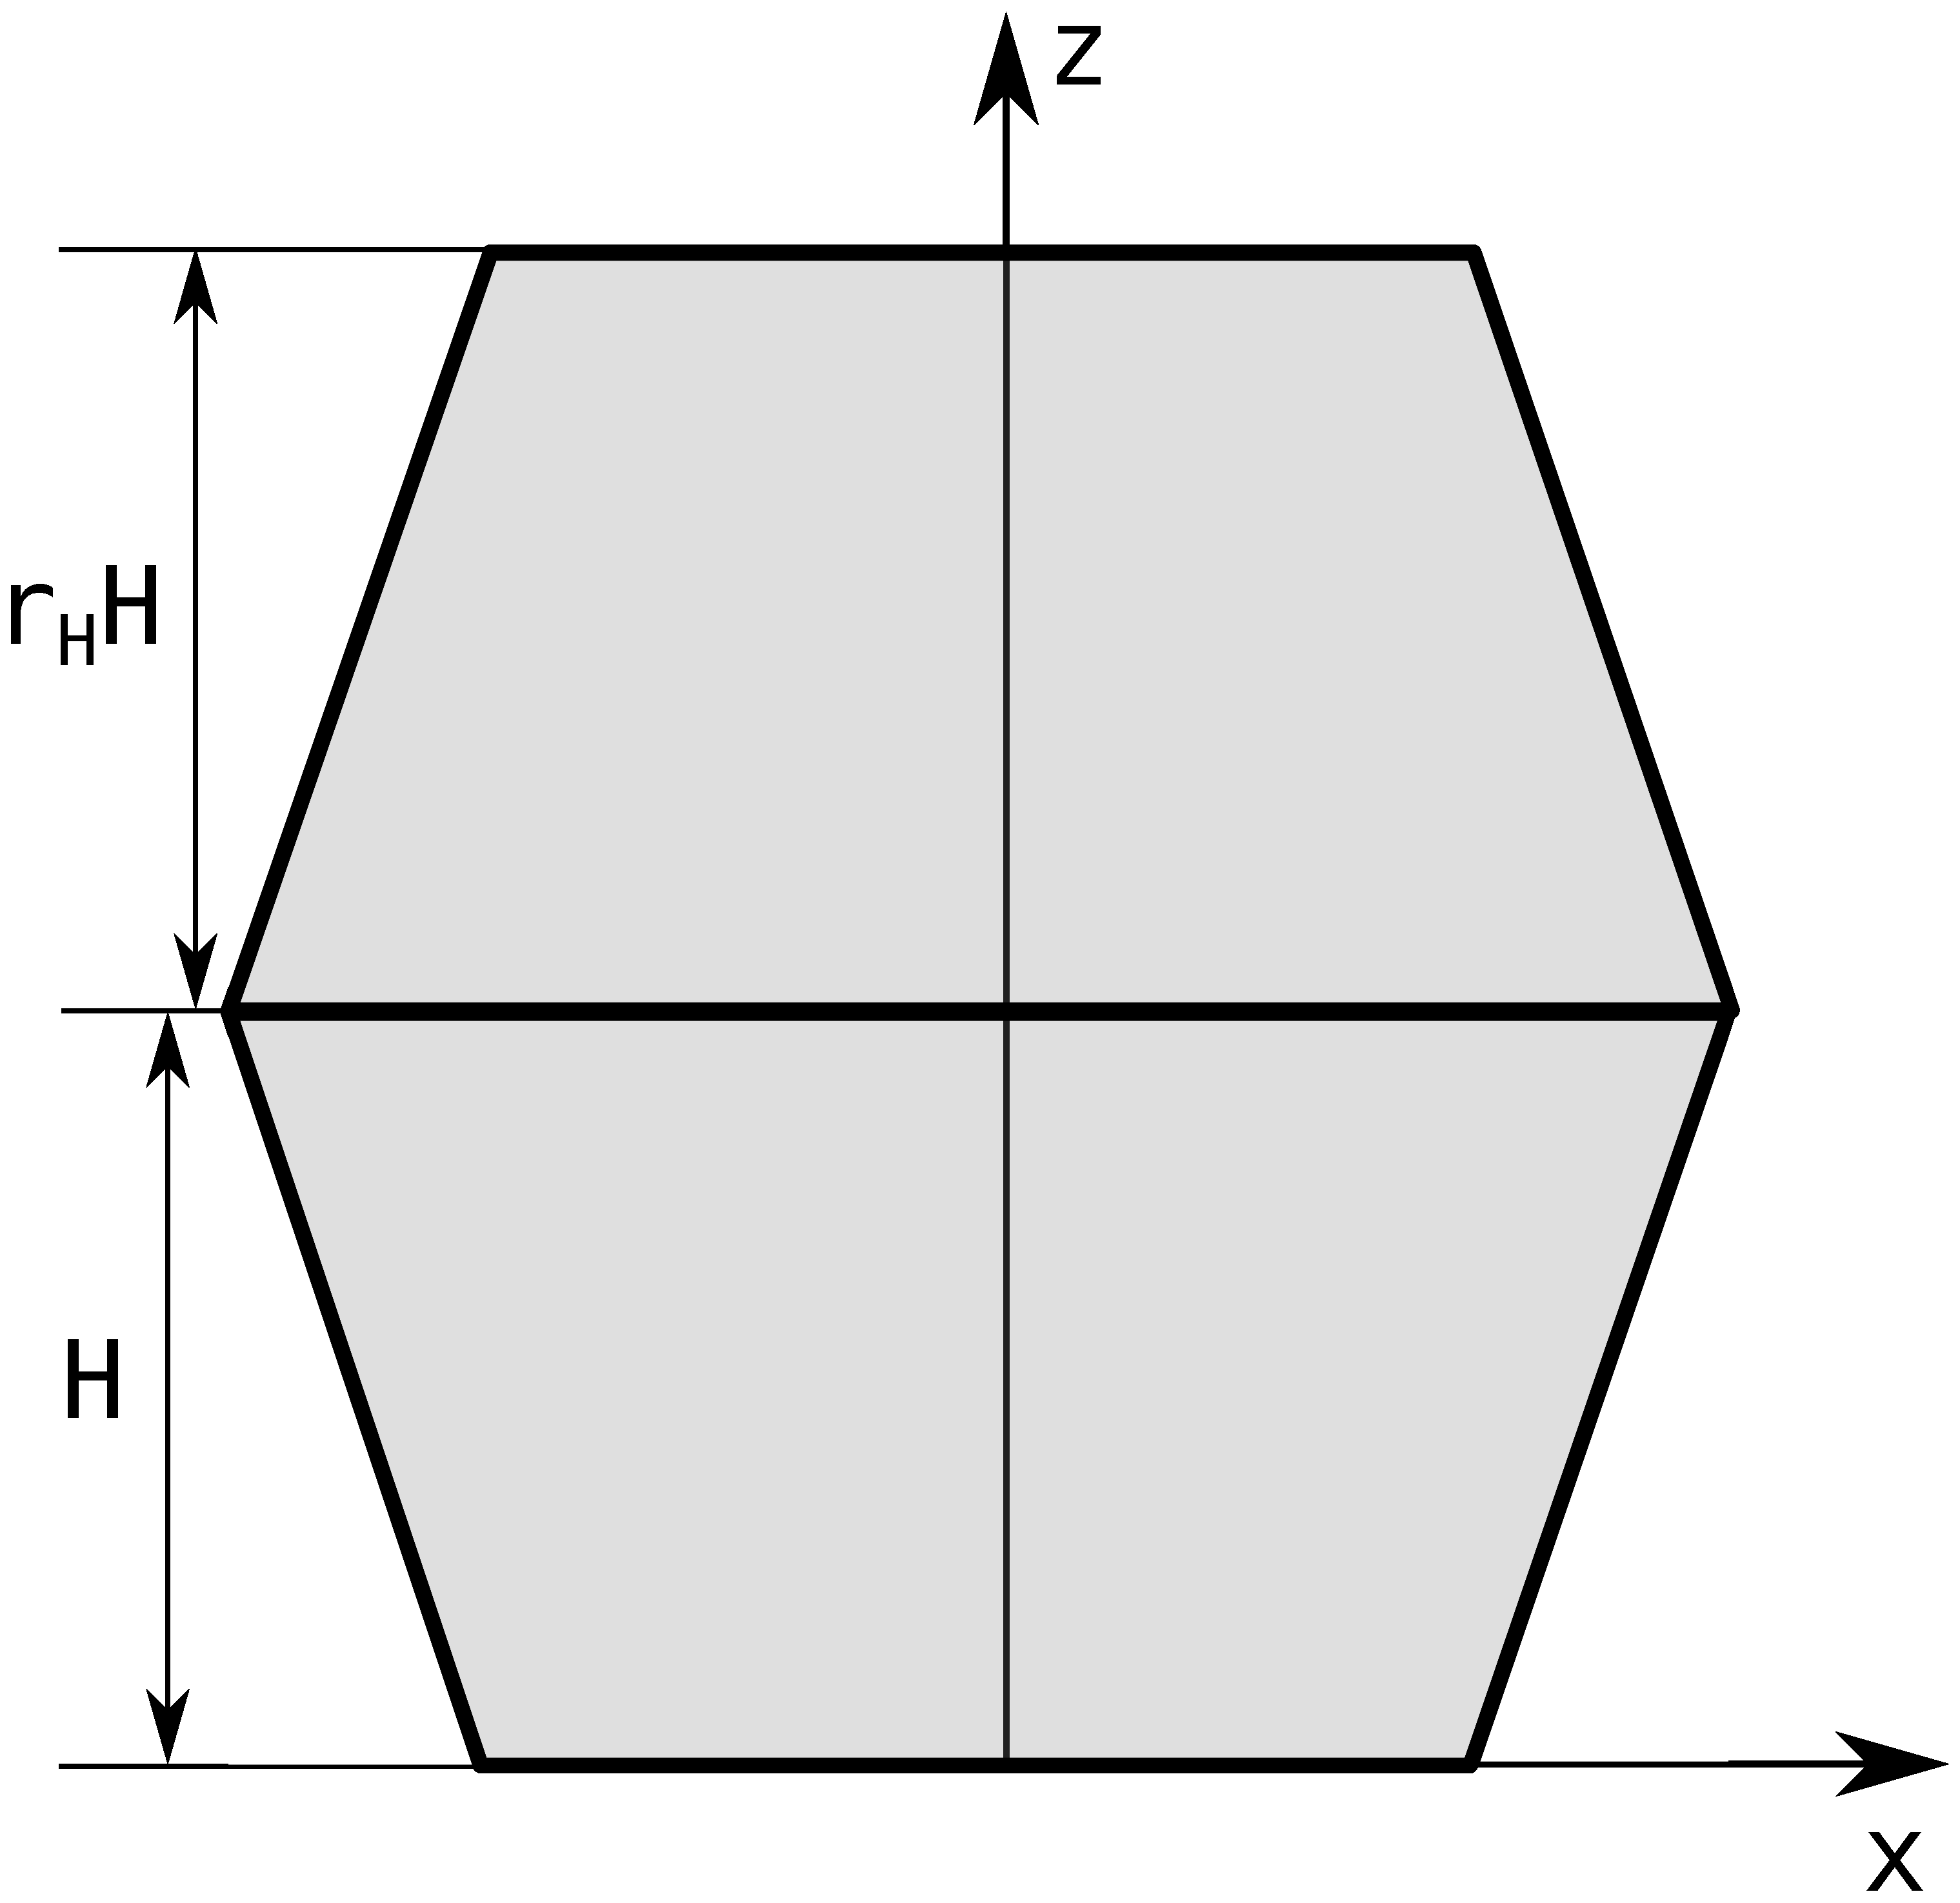
\includegraphics[width=5cm]{Figures/Cuboctahedron2dxz}}
\hfill
\subfigure[Top view]{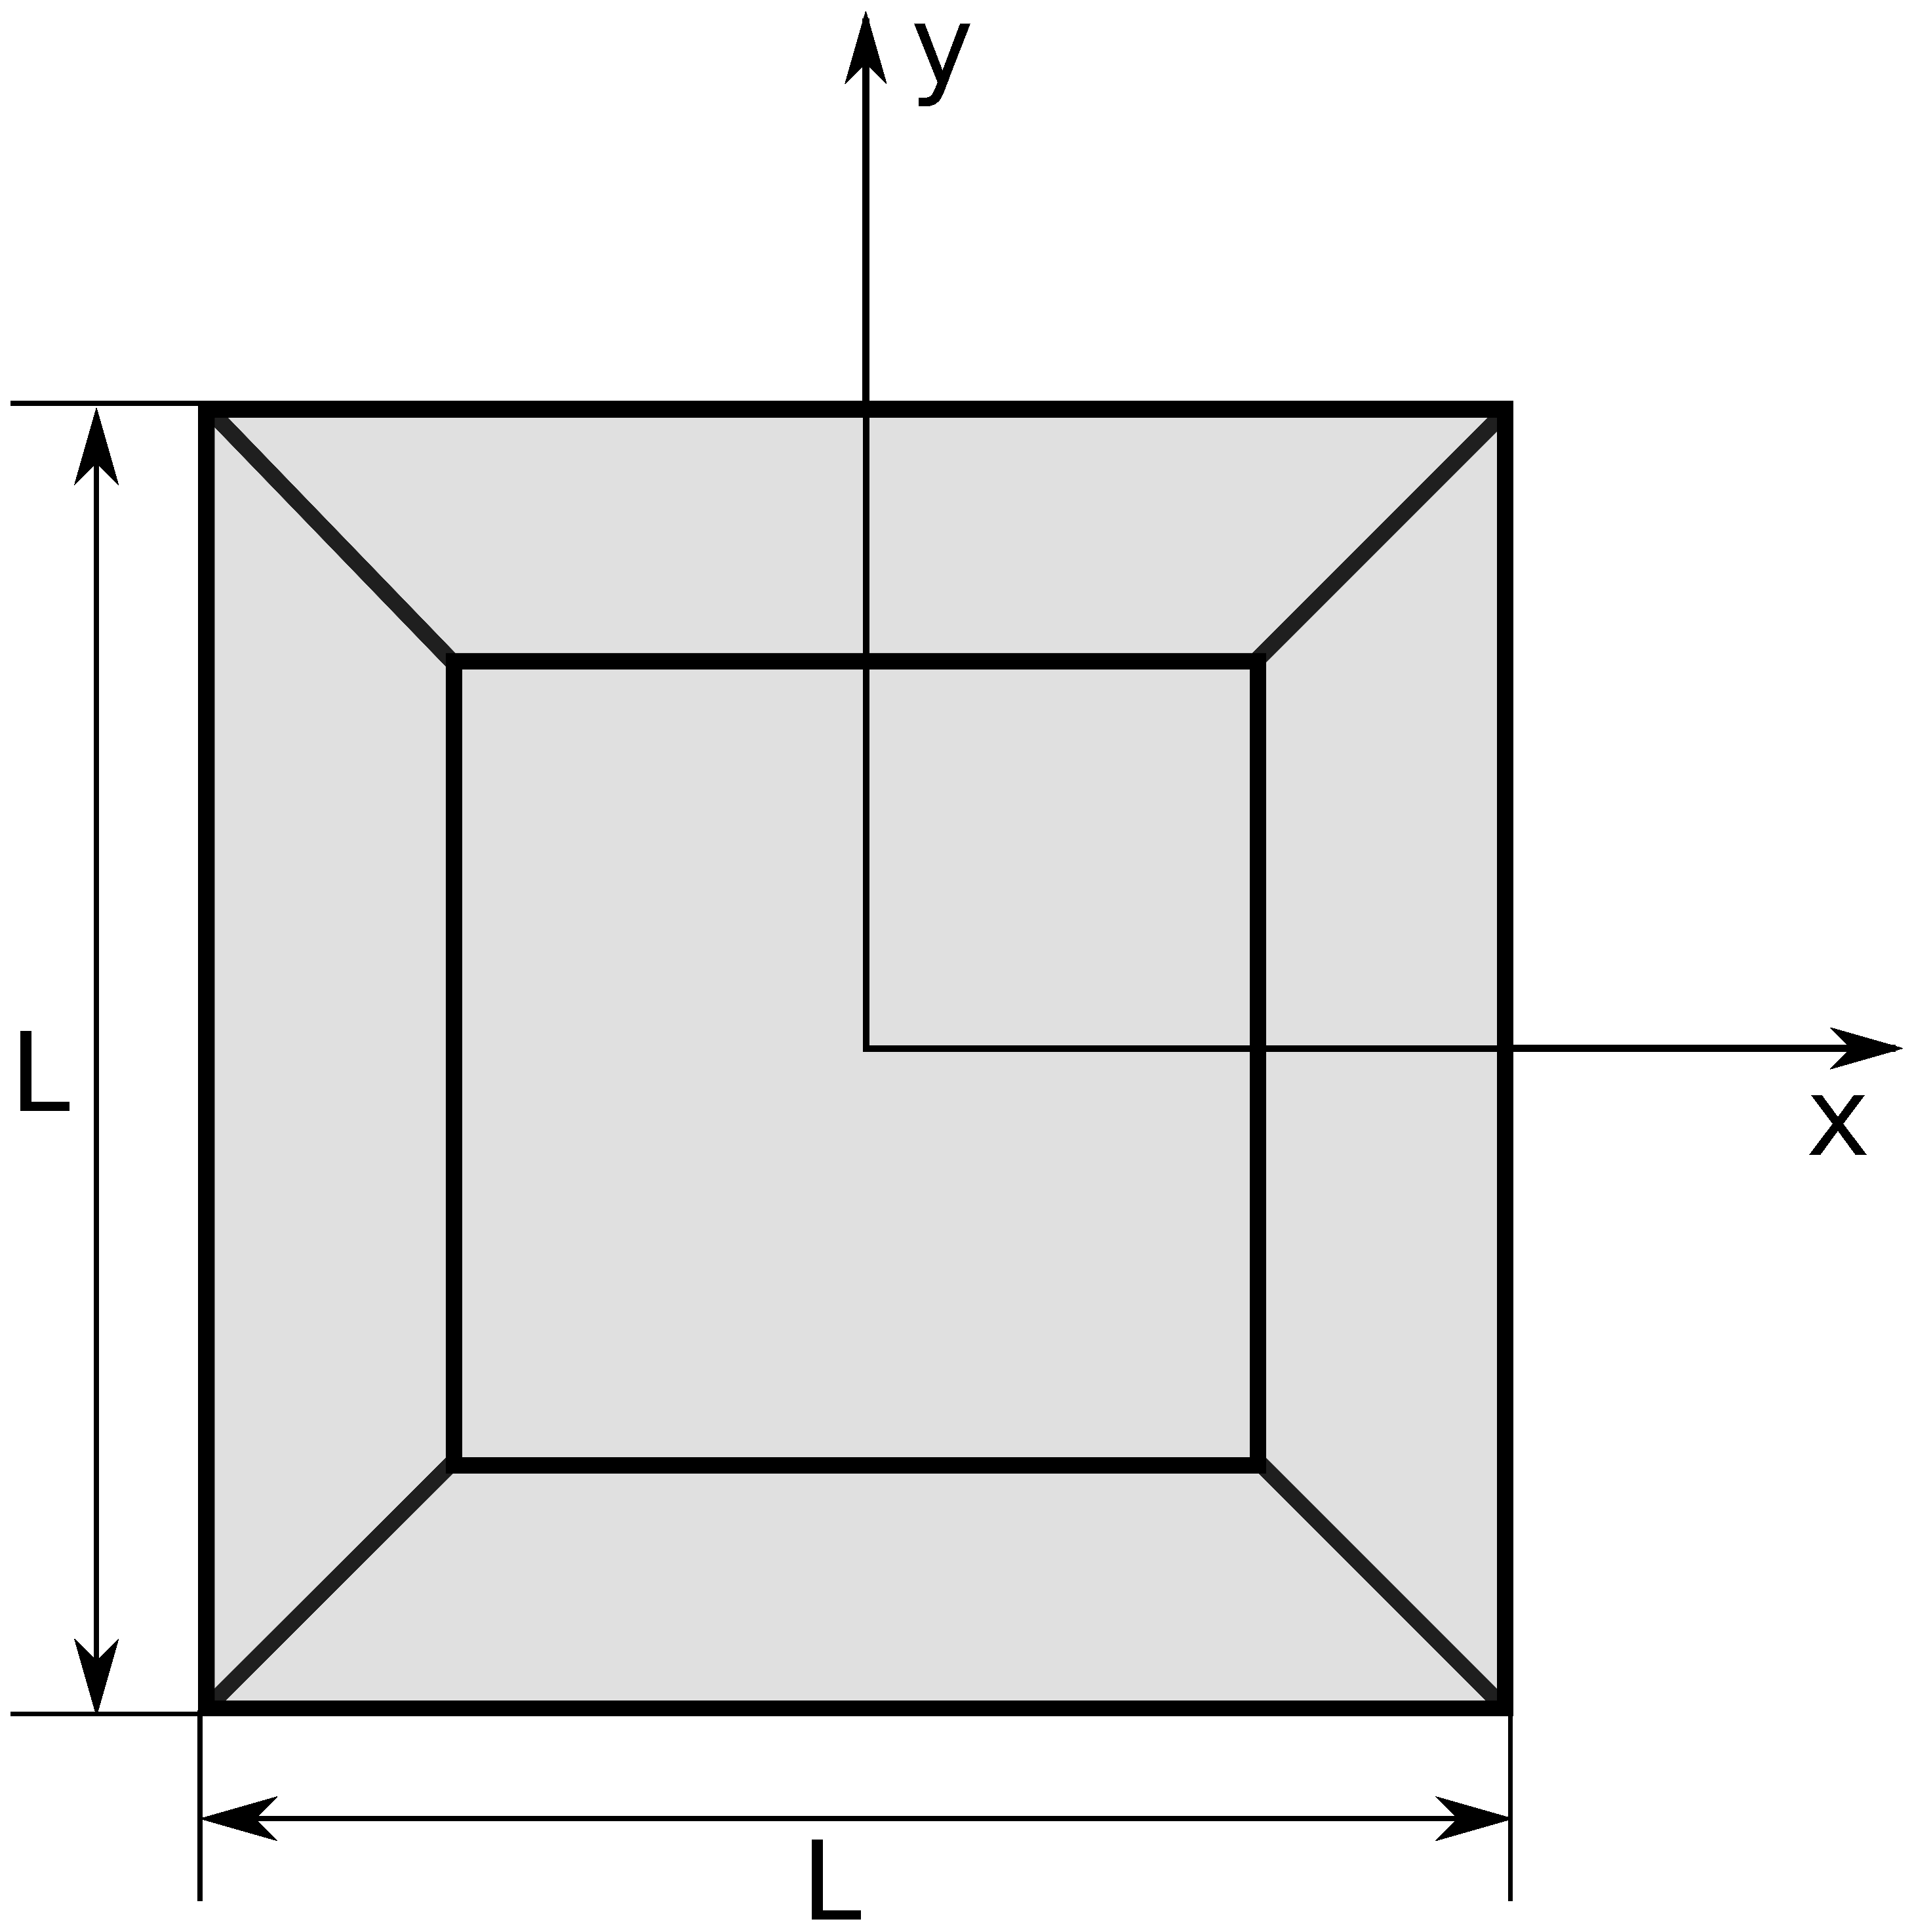
\includegraphics[width=5cm]{Figures/Cuboctahedron2dxy}}
\hfill
\caption{Sketch of a Cuboctahedron.}
\label{fig:cuboctahedron}
\end{figure}

\FloatBarrier

\paragraph{Parameters:}
\begin{itemize}
\item length of the shared square base $L$,
\item height $H$,
\item height\_ratio $r_H$,
\item $\alpha$ is the angle between the base and the
  side faces, taken in the middle of the base lines (see
  fig.~\ref{fig:pyramid} in \SecRef{Pyramid}).
\end{itemize}

\paragraph{Restrictions on the parameters:} $\dfrac{2H}{L}< \tan(\alpha)$ and $\dfrac{2r_HH}{L}< \tan(\alpha)$.

\paragraph{Properties:}
\begin{itemize}
\item volume $ V= \dfrac{1}{6} \tan(\alpha)L^3 \Big[ 2
         - \Big(1 - \dfrac{2H }{L\tan(\alpha)} \Big)^3
           - \Big(1 - \dfrac{2 r_H
             H}{L\tan(\alpha) }\Big)^3\Big]$,
\item particle surface seen from above $S =L^2$.
%\item radius of gyration
\end{itemize}

\subsection{Expression of the form factor}
\begin{equation*}
F_{\rm{Cuboctahedron}}(\mathbf{q}, L, H, r_H, \alpha)=\exp(iq_z
H)\Big[F_{\rm{Pyramid}}(q_x,q_y, q_z, L, r_H H,
\alpha)+F_{\rm{Pyramid}}(q_x, q_y, -q_z, L, H, \alpha))\Big]
\end{equation*}

\paragraph{Syntax:} \Code{FormFactorCuboctahedron(length, height, height\_ratio,
  alpha)}

\subsection{Examples}
Figure~\ref{fig:FFcuboctahEx} shows the normalized intensity $|F|^2/V^2$, computed with $L=20$~nm, $H=13$~nm, $r_H=0.7$, and $\alpha=60^{\circ}$.
\begin{figure}[h]
\begin{center}
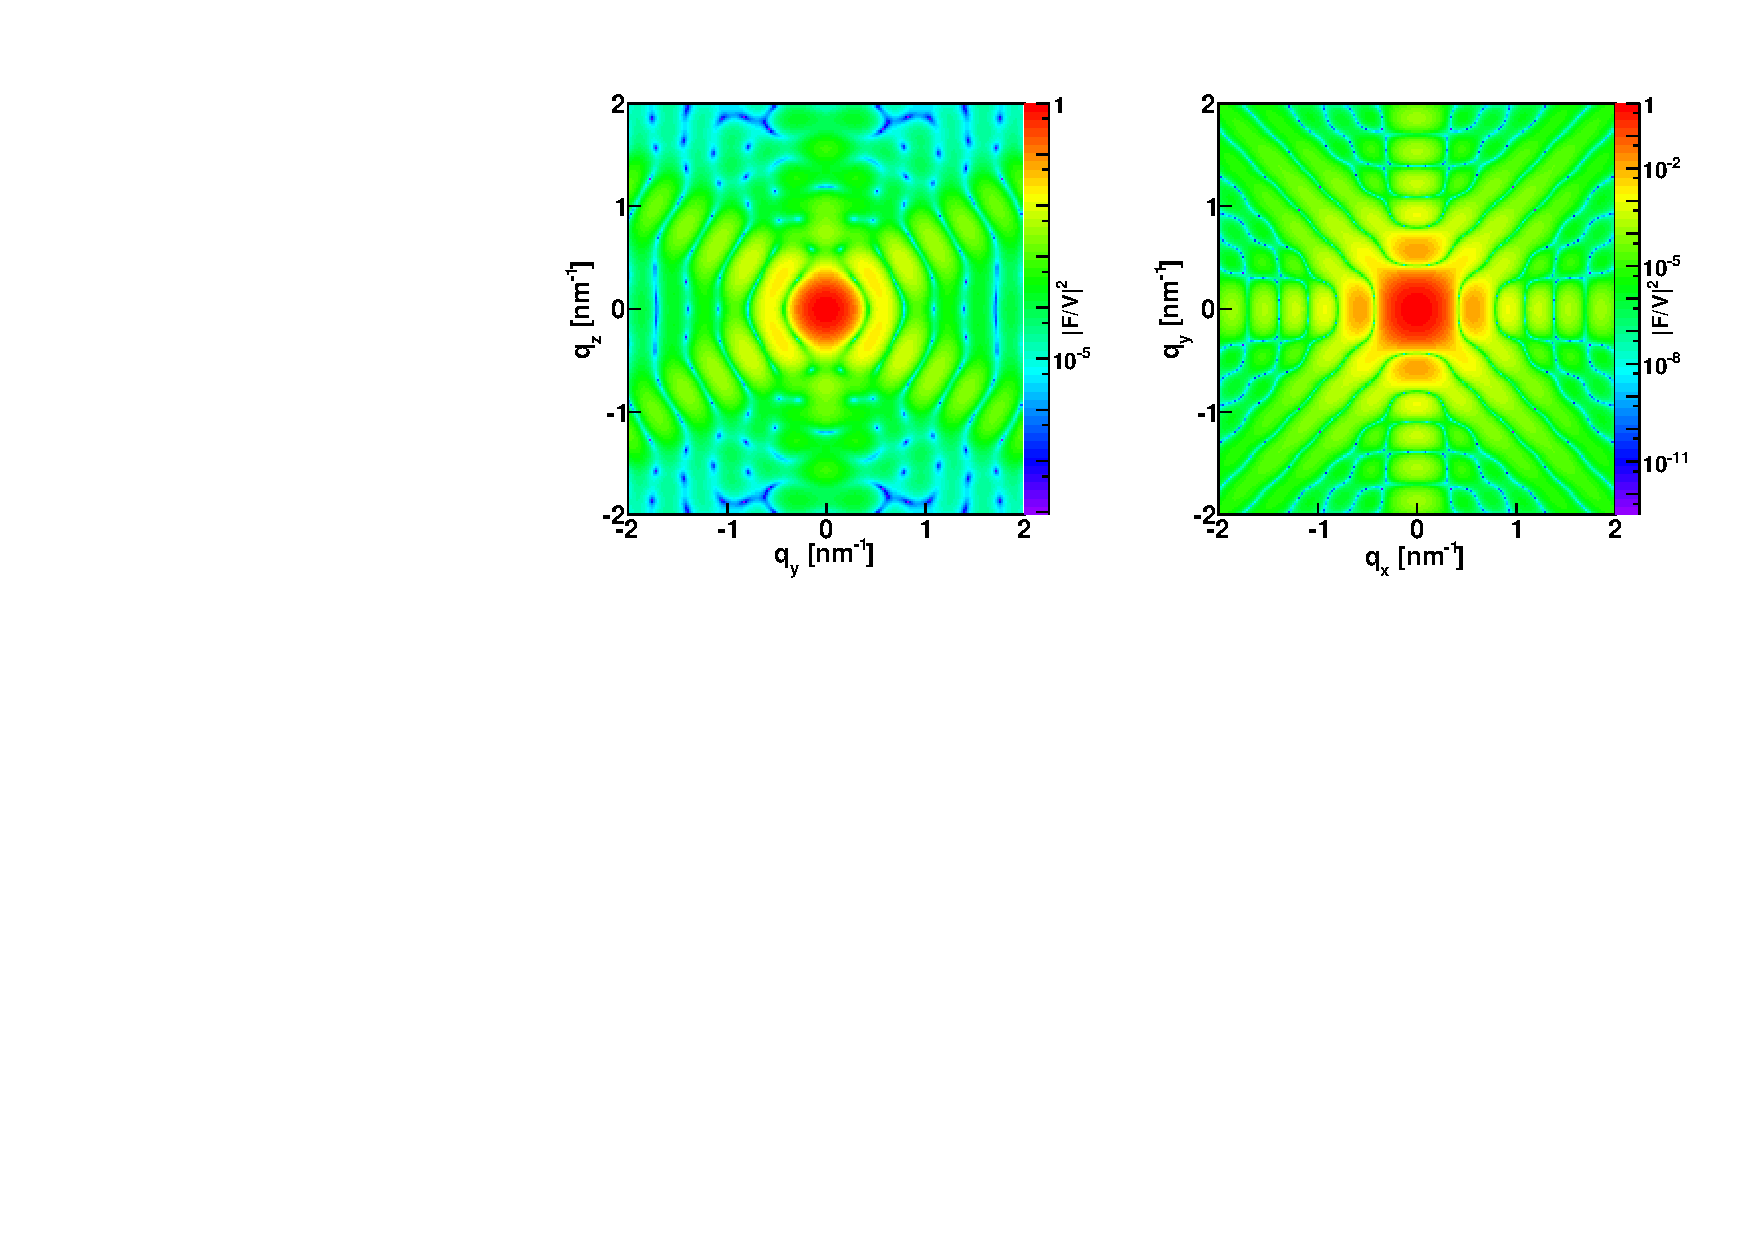
\includegraphics[width=\textwidth]{Figures/figffcuboctah}
\end{center}
\caption{Normalized intensity for the form factor of a cuboctahedron $|F|^2/V^2$, plotted against ($q_z$, $q_y$) and  ($q_x$, $q_y$) and computed with $L=20$~nm, $H=13$~nm,
  $r_H=0.7$, and $\alpha=60^{\circ}$.}
\label{fig:FFcuboctahEx}
\end{figure}

\FloatBarrier

%\subsection{References}
%In comparison with \Code{IsGISAXS}, as for the  form factor of a  Pyramid,
%we use the full length of a side of the square base:
%$L=2R_{\rm{\Code{IsGISAXS}}}$. 

\newpage{\cleardoublepage}
%%%%%%%%%%%%%%%%%%%%%%%%%%%%%%%%%%%%	
\section{Cylinder} \SecLabel{Cylinder}
 
\subsection{Real-space geometry}
This shape is a right circular cylinder (see fig.~\ref{fig:cylinder}).

\begin{figure}[ht]
\hfill
\subfigure[Side view]{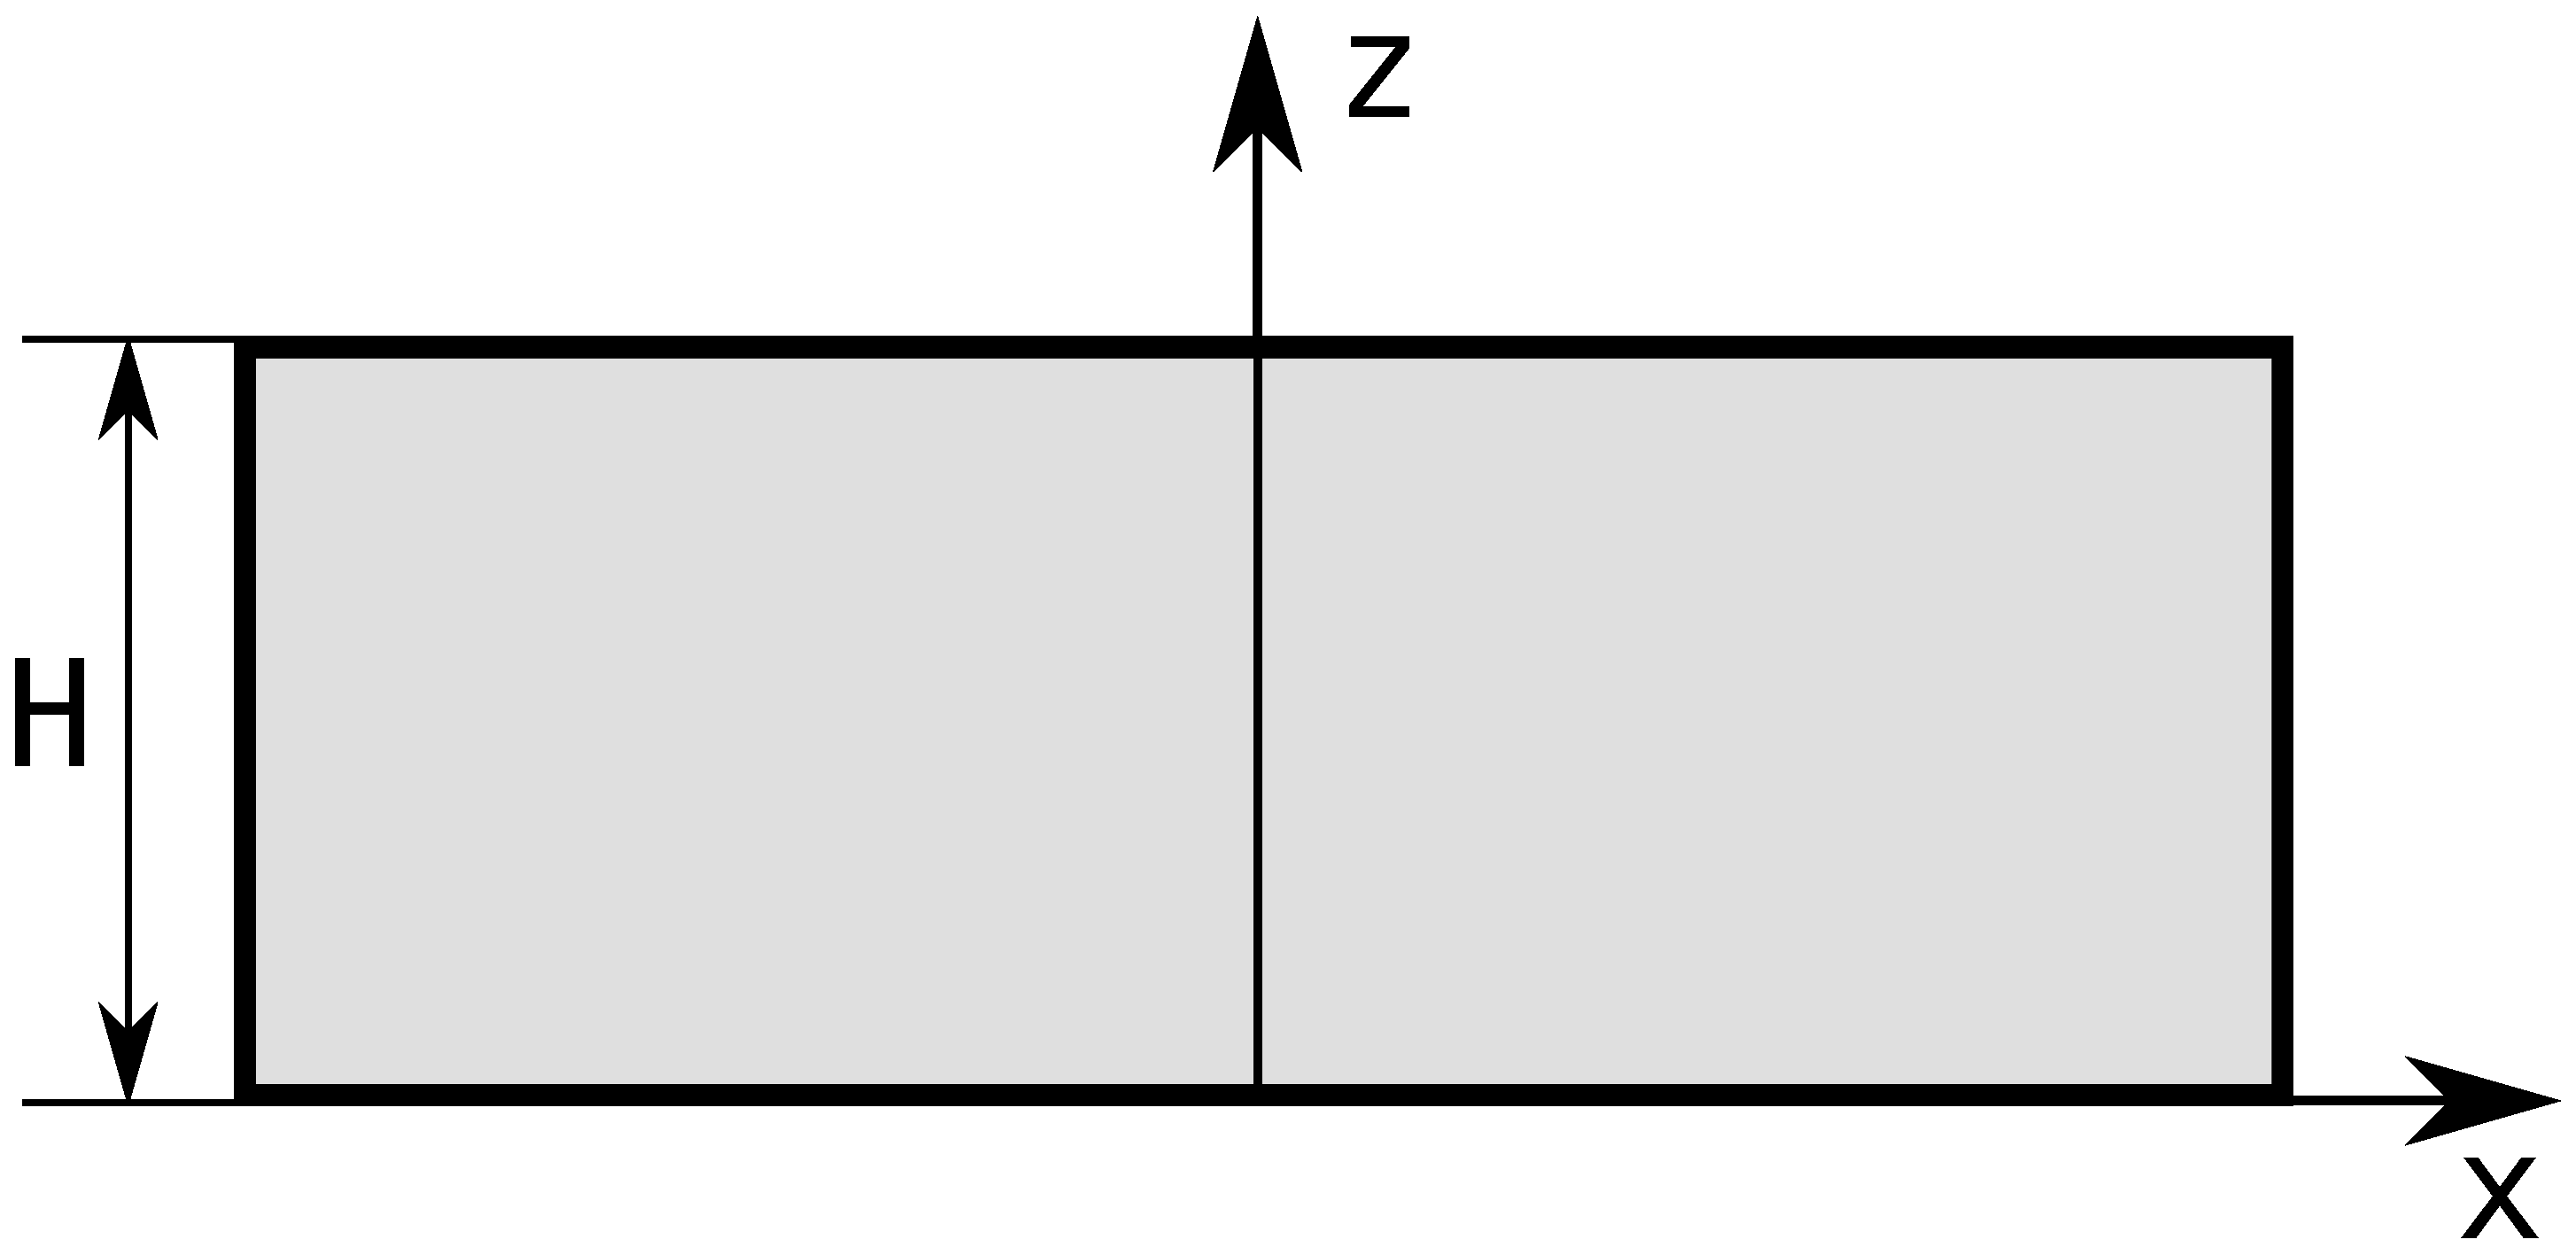
\includegraphics[width=5cm]{Figures/Cylinder2dxz}}
\hfill
\subfigure[Top view]{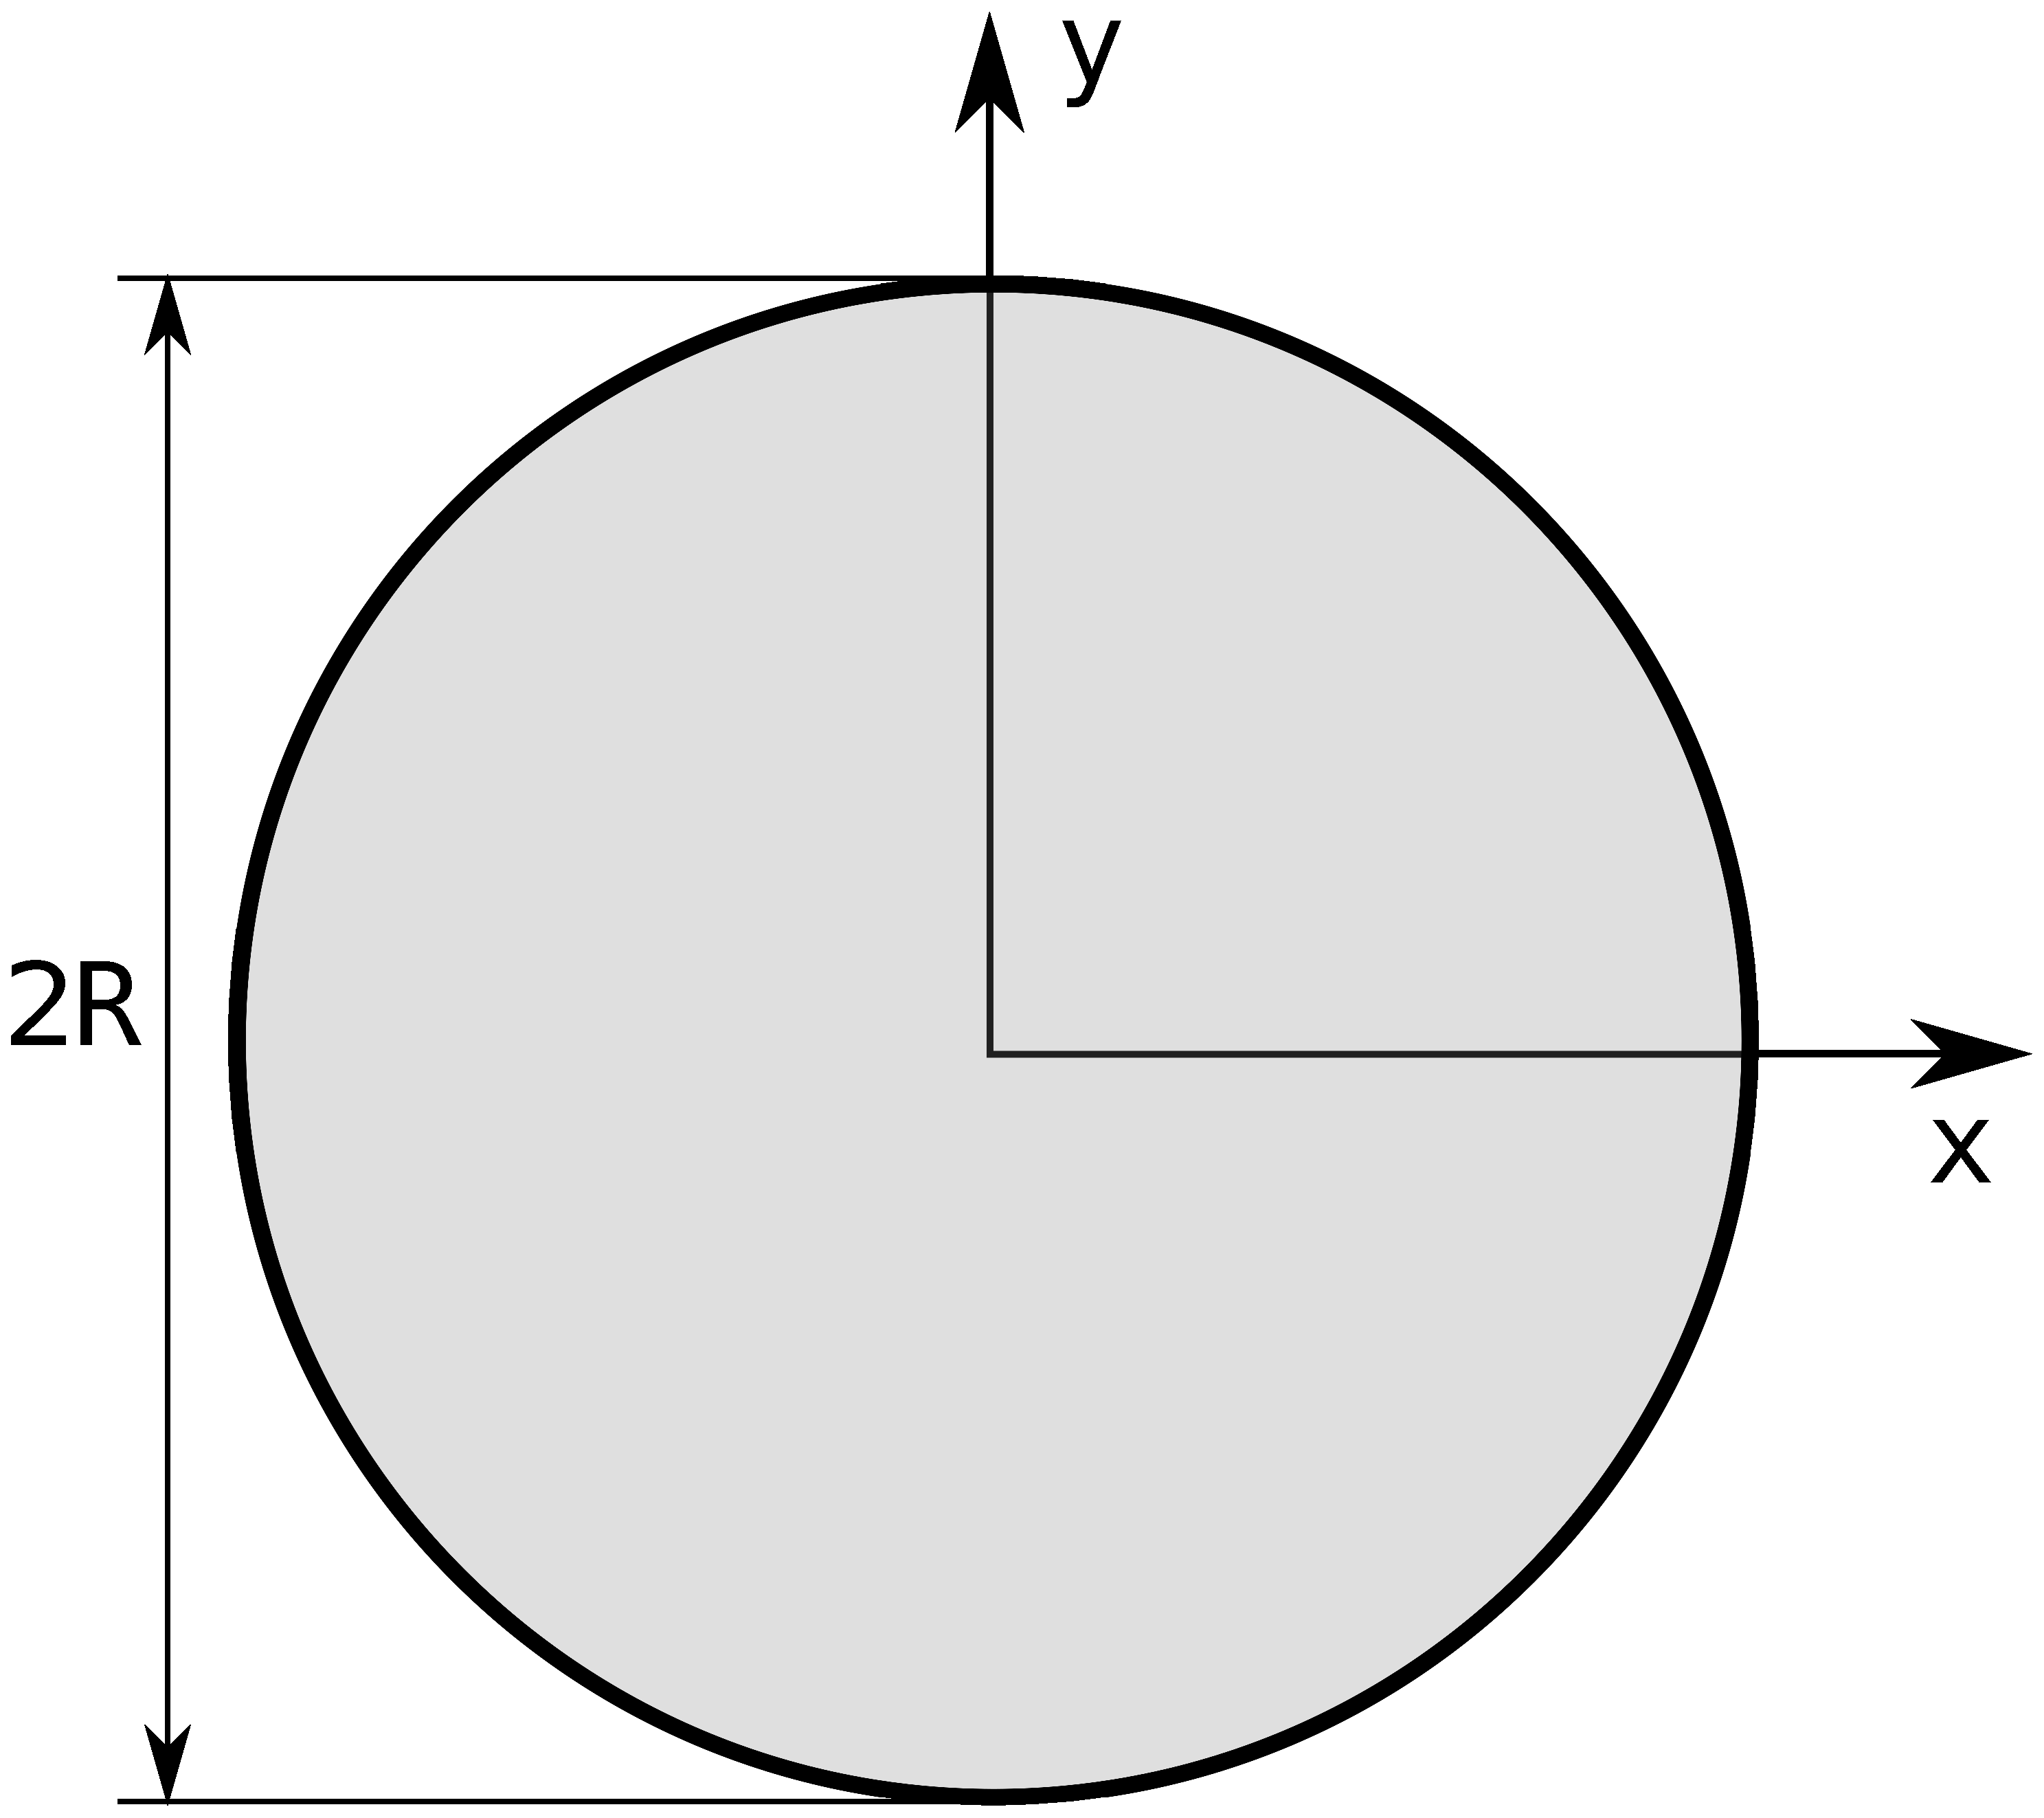
\includegraphics[width=5cm]{Figures/Cylinder2dxy}}
\hfill
\caption{Sketch of a Cylinder.}
\label{fig:cylinder}
\end{figure}

\paragraph{Parameters:}
\begin{itemize}
\item radius of the circular base $R$. 
\item height $H$.
\end{itemize}

\paragraph{Properties:}
\begin{itemize}
\item volume $V = \pi R^2 H$,
\item particle surface seen from above $S=\pi R^2$.
%\item radius of gyration
\end{itemize}

\subsection{Expression of the form factor}
  \begin{equation*}
F_{\rm{Cylinder}}(\mathbf{q},R, H)=  2\pi
 R^2 H  \sinc\left(q_ z \frac{H}{2}\right) \exp\left(i q_ z \frac{H}{2}\right) \frac{J_1(q_{\parallel} R )}{q_{\parallel} R },
 \end{equation*}
with $q_{\parallel}=\sqrt{q_x^2+q_y^2}$ and $J_1(x)$ is the first order
Bessel function of the first kind \cite{AbSt64}.

\paragraph{Syntax:} \Code{FormFactorCylinder(radius, height)}

\newpage

\subsection{Examples}
Figure~\ref{fig:FFcylinderEx} shows the normalized intensity
$|F|^2/V^2$, computed with $R=8$~nm and \mbox{$H=16$~nm.}
\begin{figure}[h]
\begin{center}
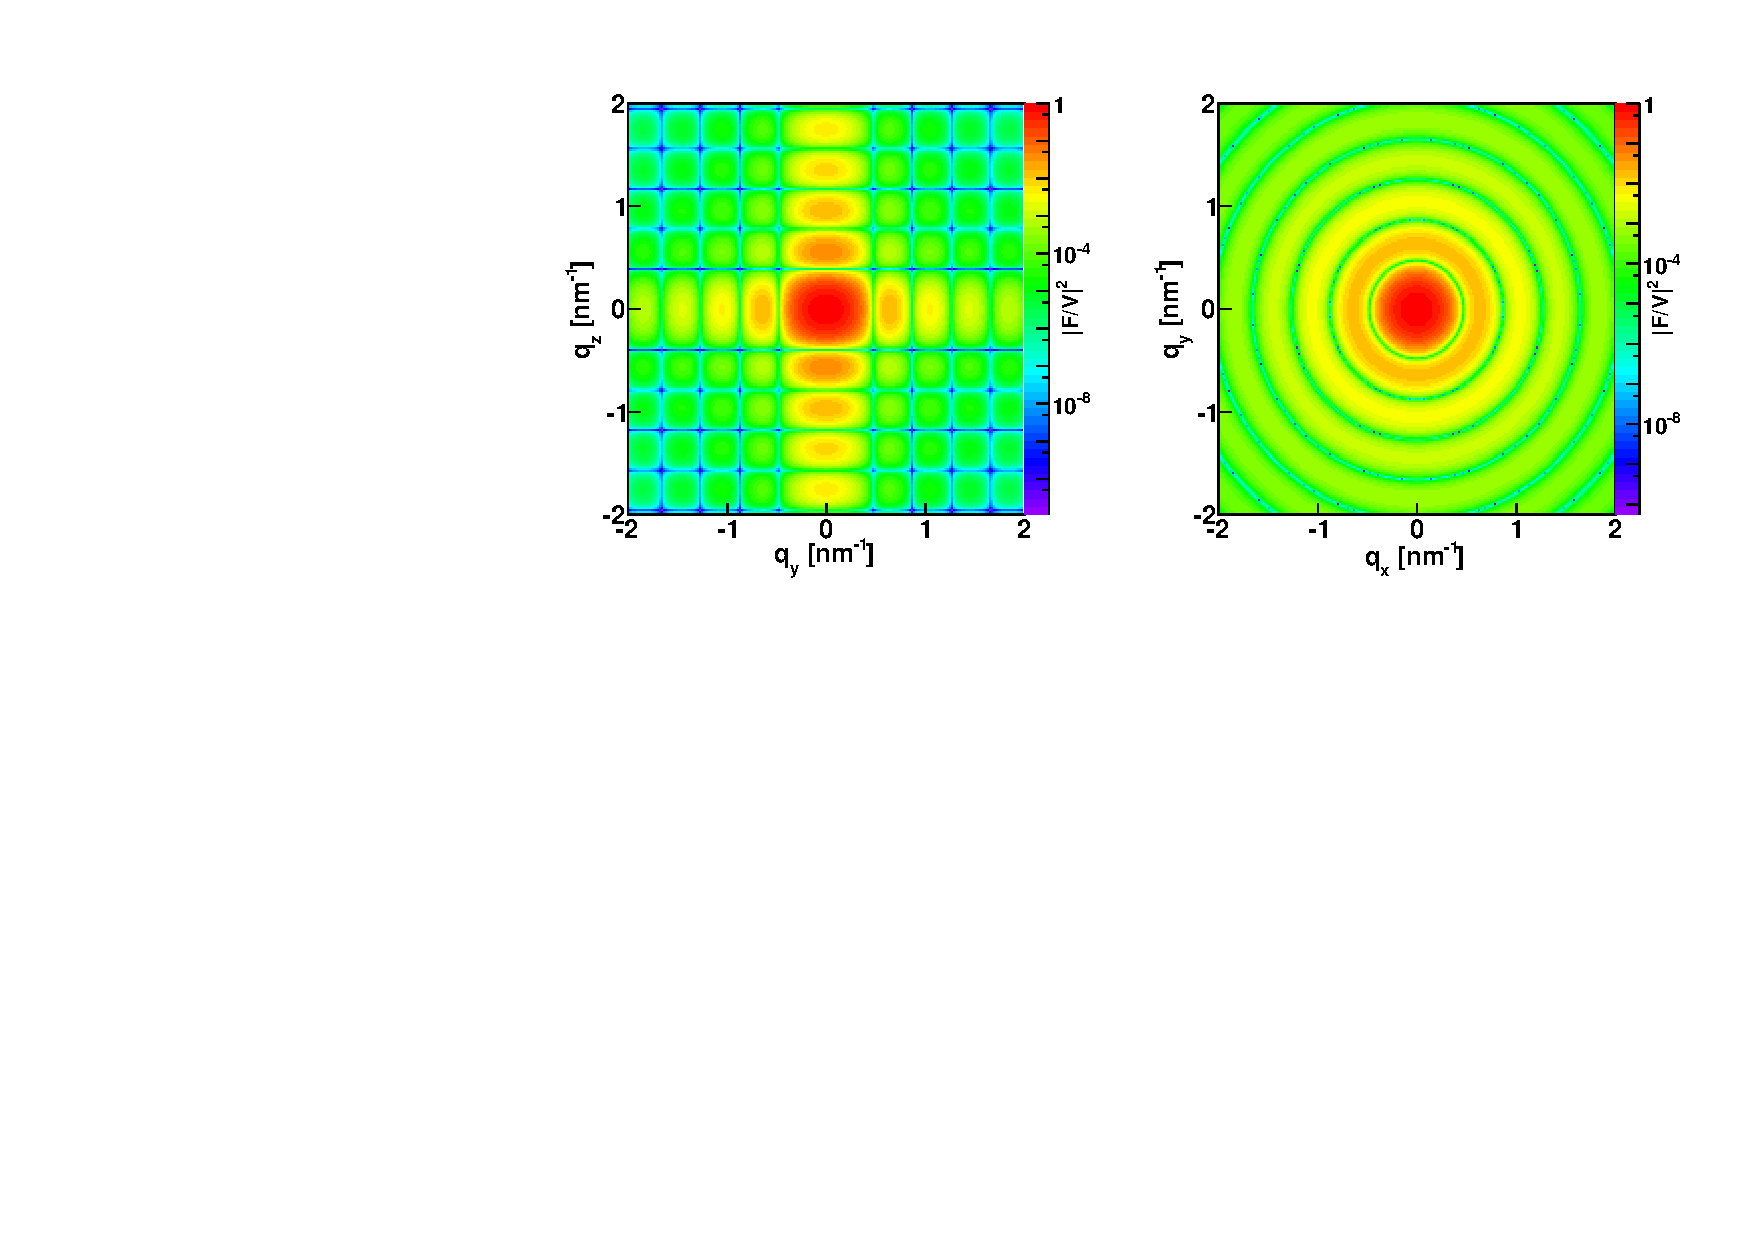
\includegraphics[width=\textwidth]{Figures/figffcylinder}
\end{center}
\caption{Normalized intensity for the form factor of a cylinder
$|F|^2/V^2$, plotted against ($q_z$, $q_y$) and  ($q_x$, $q_y$.) It
has been  computed with $R=8$~nm and $H=16$~nm.}
\label{fig:FFcylinderEx}
\end{figure}
\FloatBarrier

%\subsection{References}

\newpage{\cleardoublepage}
%%%%%%%%%%%%%%%%%%%%%%%%%%%%%%%%%%%%
\section{Ellipsoidal cylinder} \SecLabel{EllipsoidalCylinder} 

\subsection{Real-space geometry}
This is a cylinder whose cross section is an ellipse.

\begin{figure}[ht]
\hfill
\subfigure[Side view]{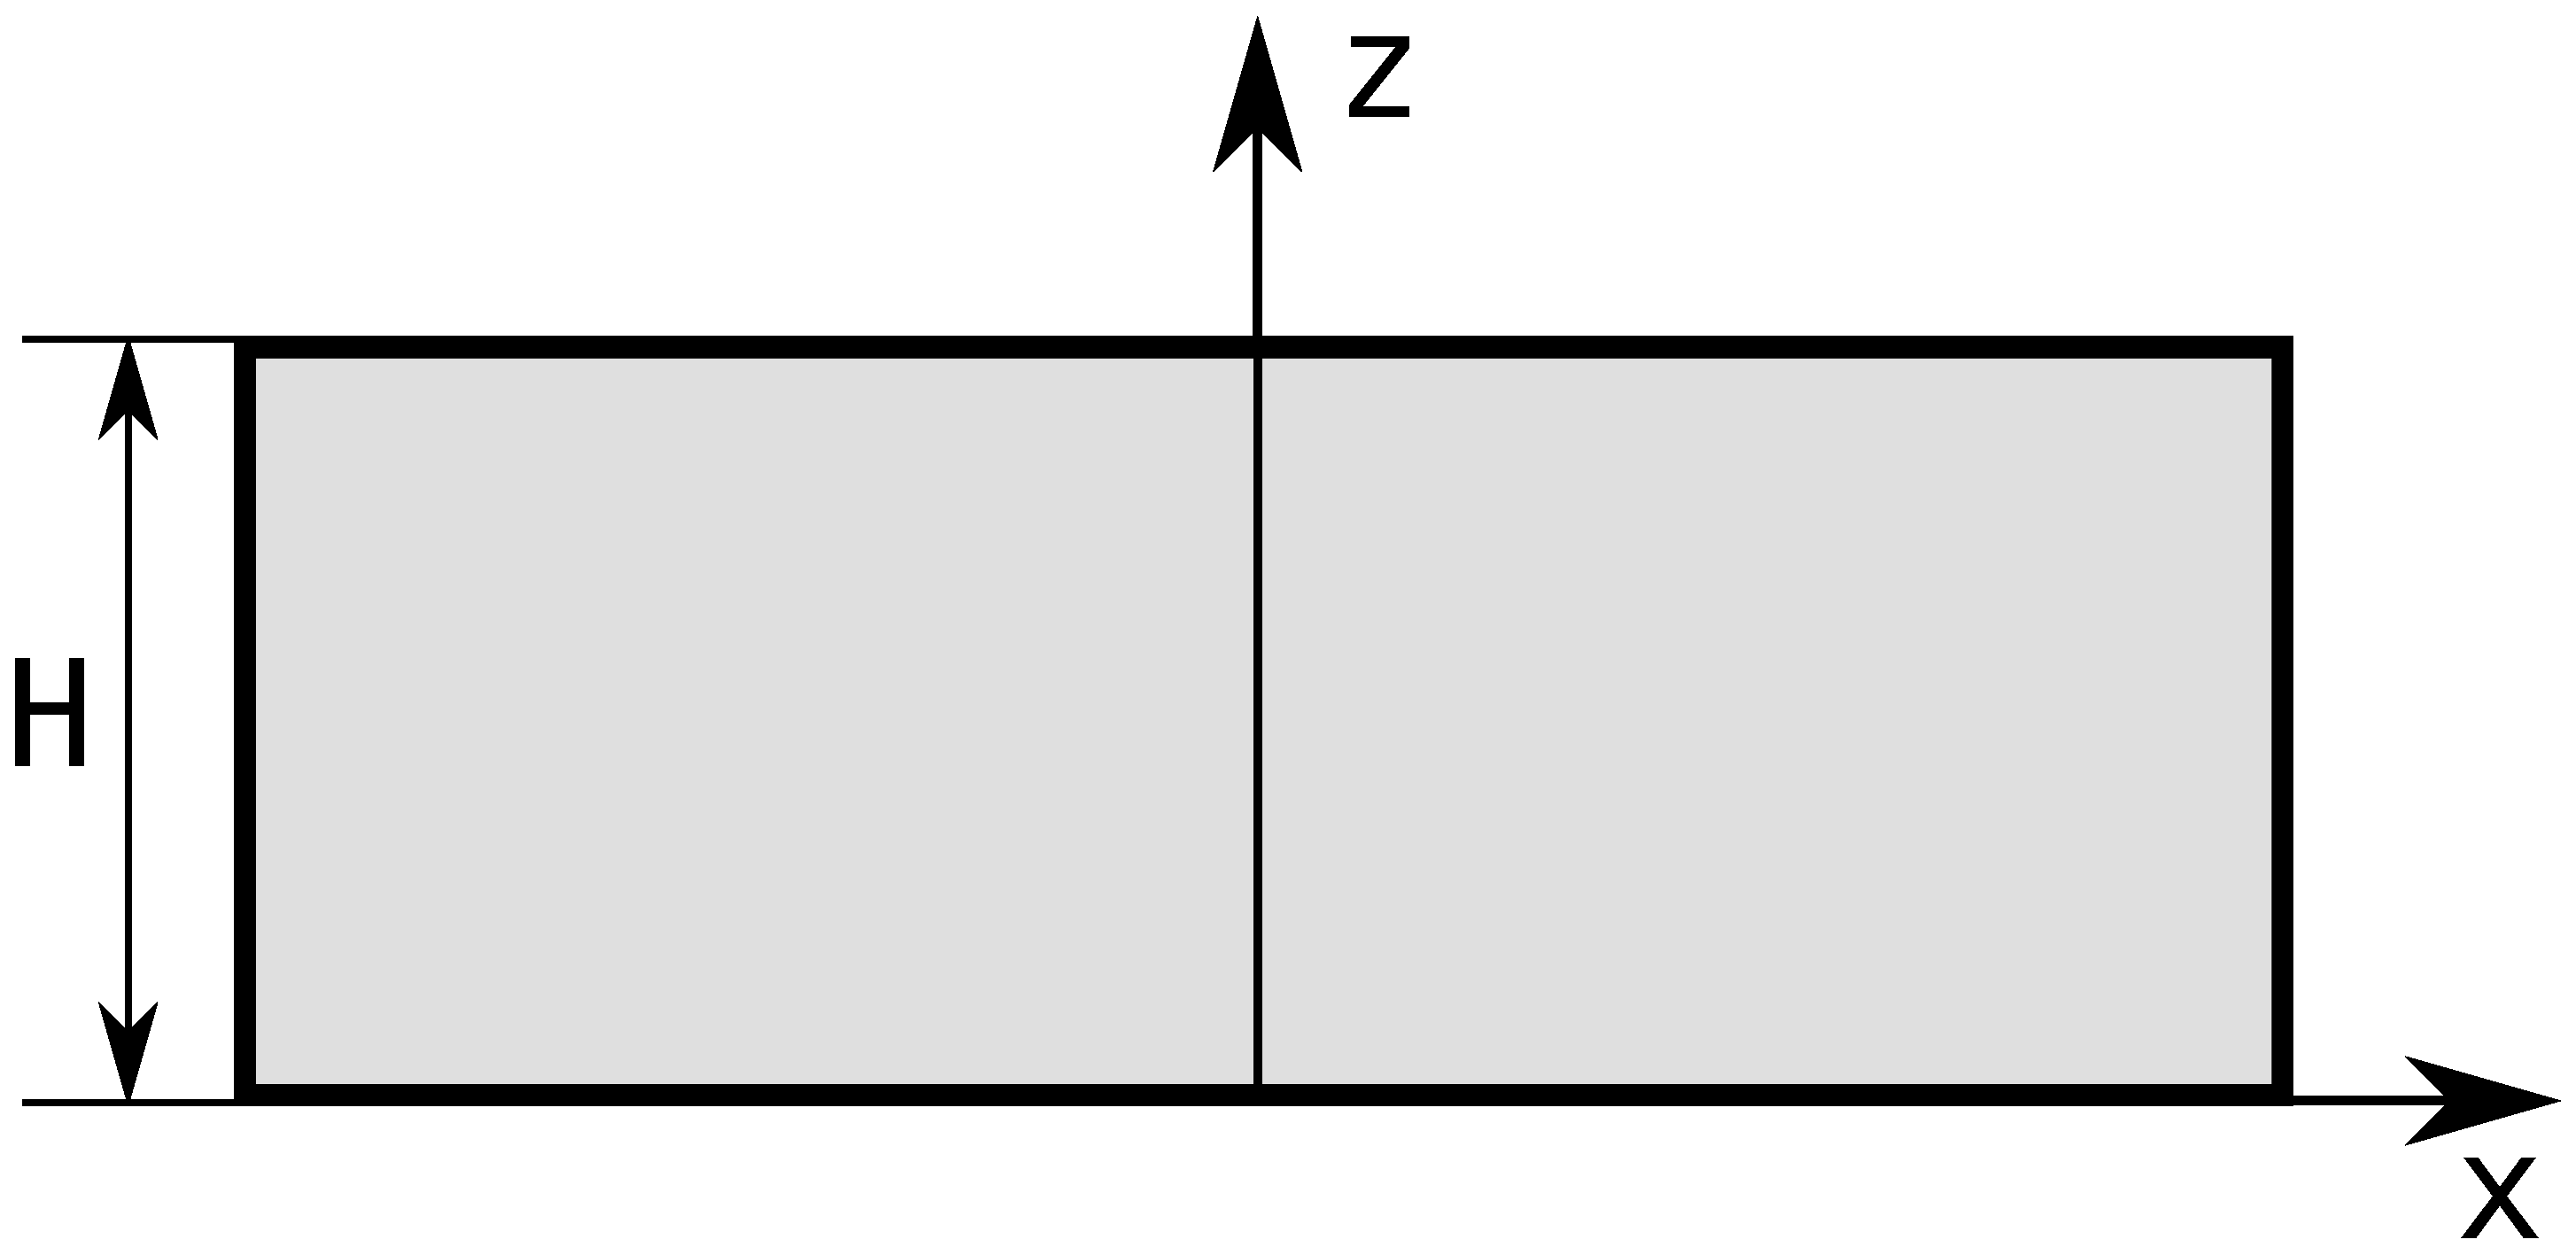
\includegraphics[width=5cm]{Figures/EllipsoidalCylinder2dxz}}
\hfill
\subfigure[Top view]{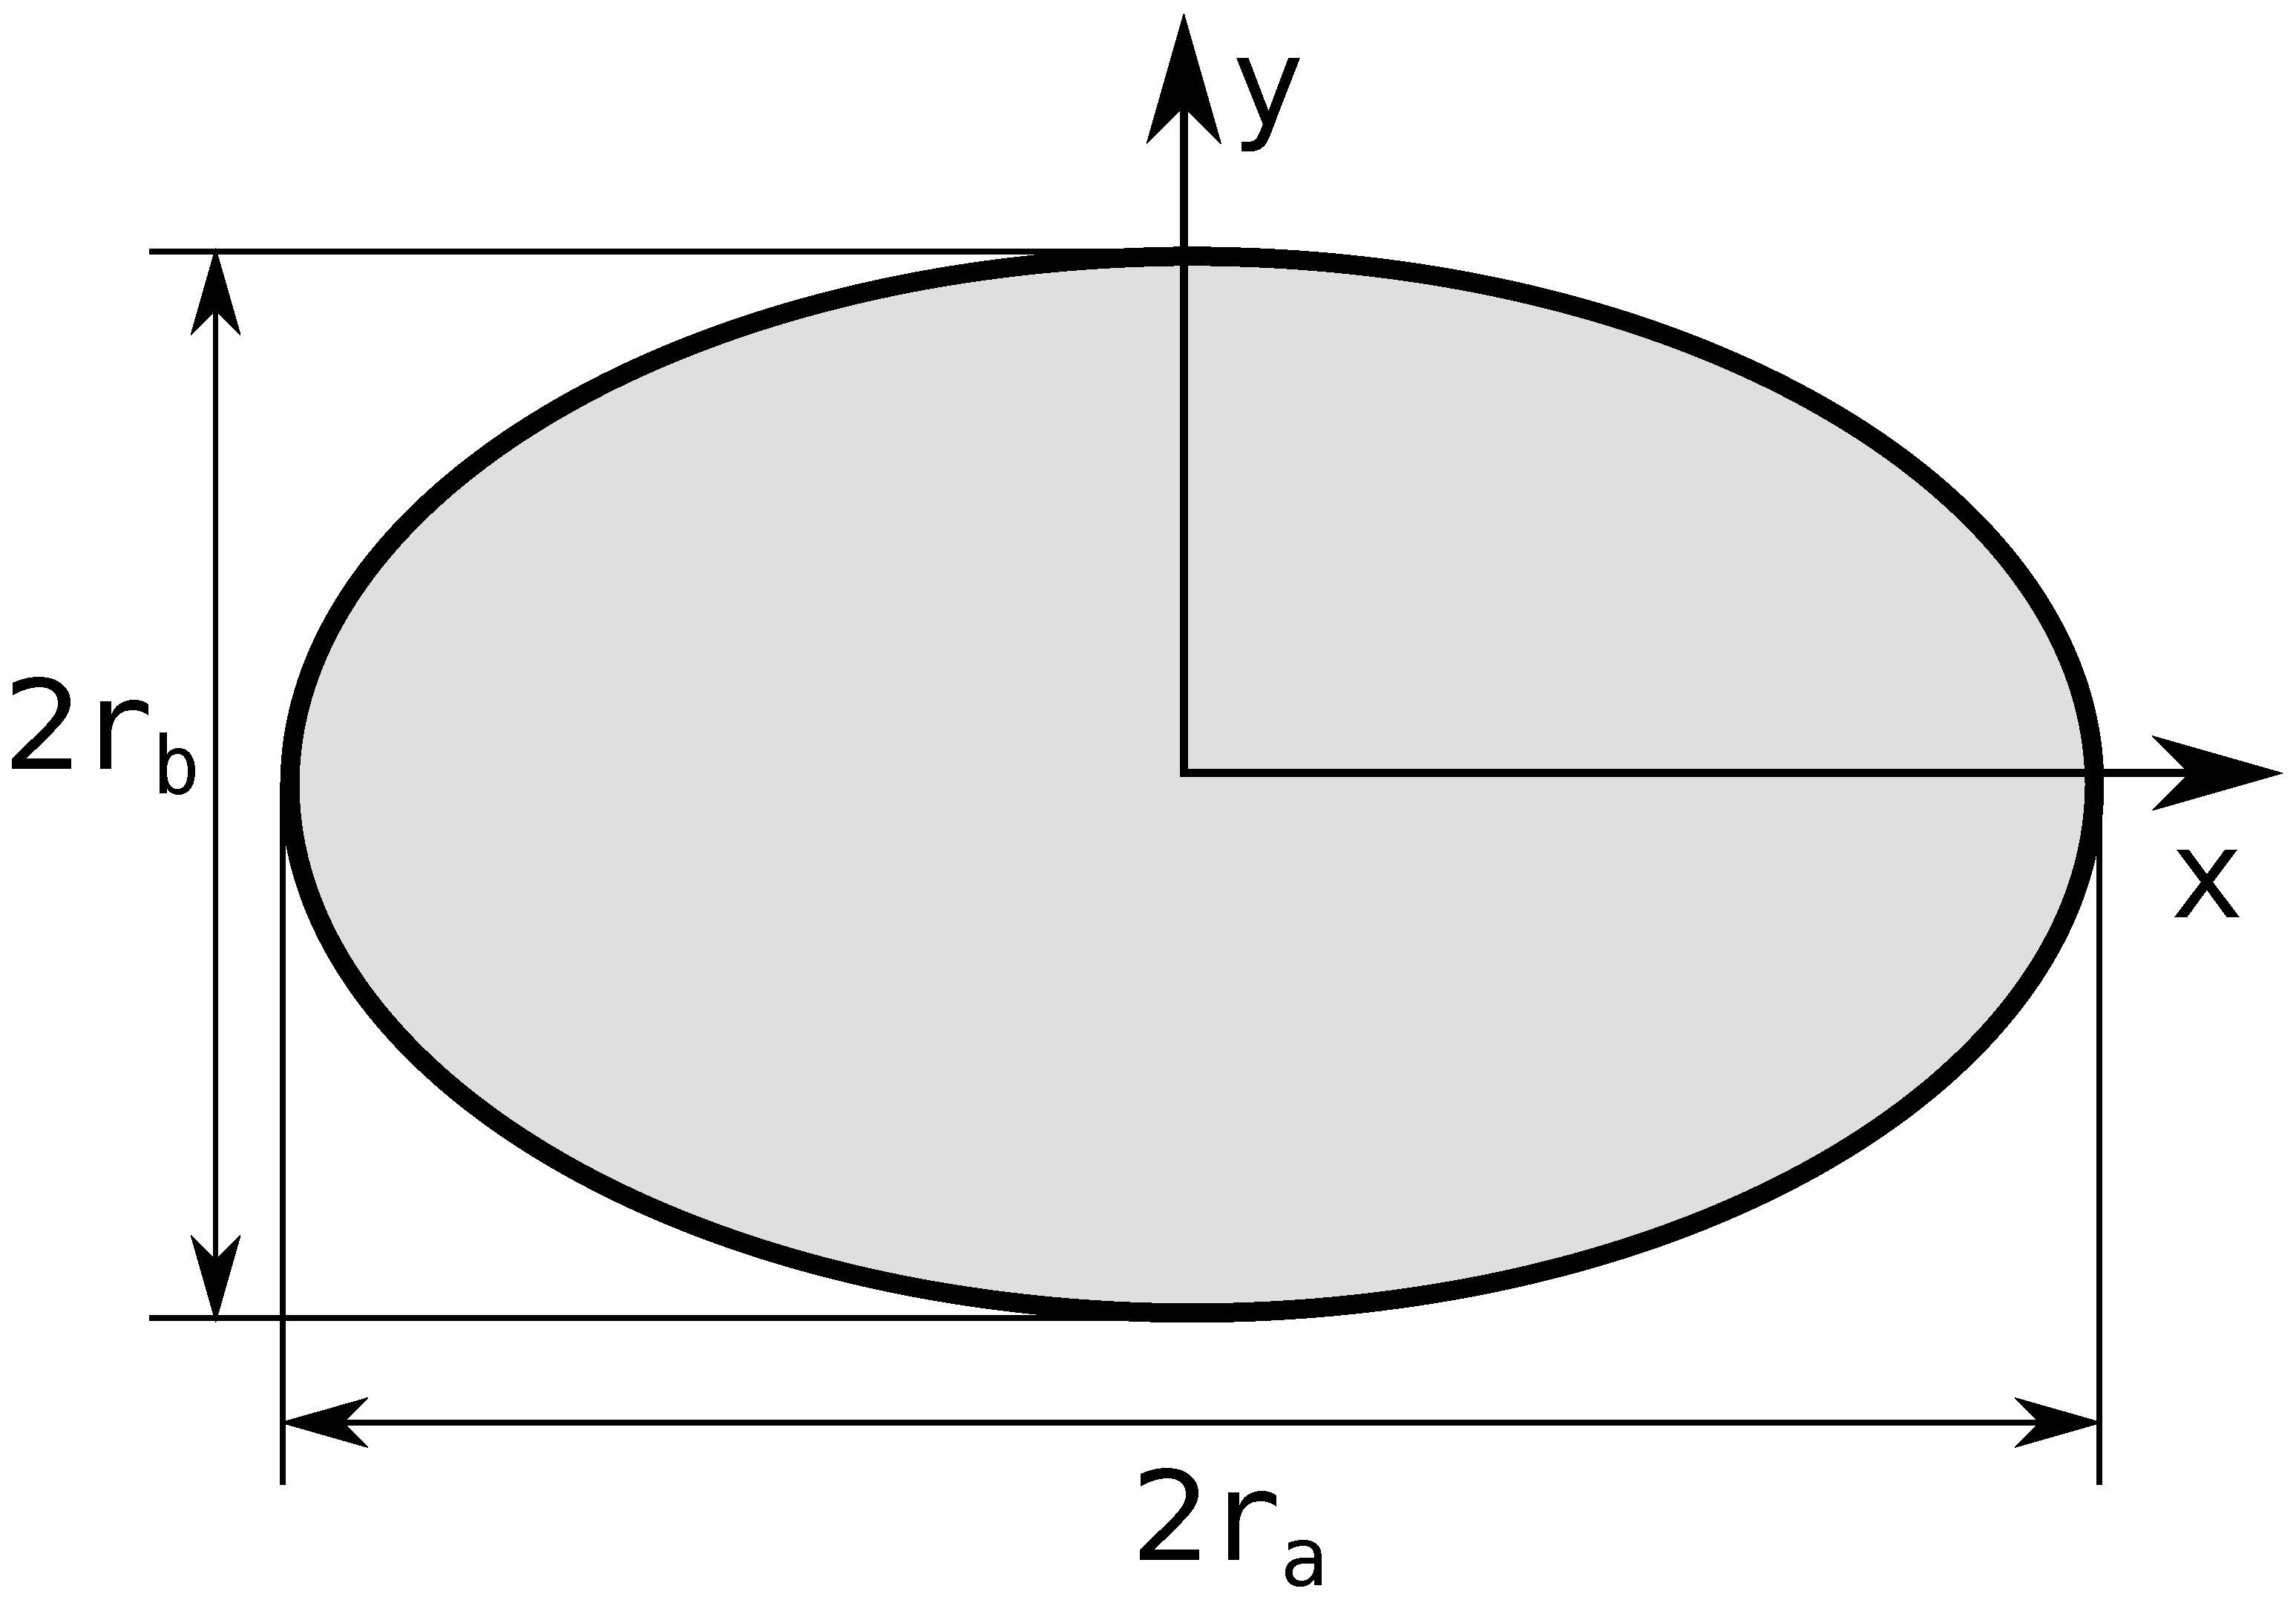
\includegraphics[width=5cm]{Figures/EllipsoidalCylinder2dxy}}
\hfill
\caption{Sketch of an Ellipsoidal Cylinder.}
\label{fig:ellipscylinder}
\end{figure}

\paragraph{Parameters:}
\begin{itemize}
\item $r_a$ = half length of the ellipse main axis parallel to $x$,
\item$r_b$ = half length of the ellipse main axis parallel to $y$, 
\item height $H$.
\end{itemize}

\paragraph{Properties:}
\begin{itemize}
\item volume $V = \pi r_a r_bH$,
\item particle surface seen from above $S = r_a r_b$.
%\item radius of gyration
\end{itemize}

\subsection{Expression of the form factor}
The total form factor is given by 
\begin{equation*}
F_{\rm{EllipsoidalCylinder}}(\mathbf{q},R,W,H) = 2\pi r_a r_b H \exp\left(i\frac{q_z
  H}{2}\right)\sinc\left(\frac{q_z H}{2}\right) \frac{J_1(\gamma)}{\gamma},
\end{equation*}
with $\gamma=\sqrt{(q_x r_a)^2+(q_y r_b)^2}$ and $J_1(x)$ is the first order
Bessel function of the first kind \cite{AbSt64}.

\paragraph{Syntax:} \Code{FormFactorEllipsoidalCylinder($r_a$, $r_b$, height)}

\newpage


\subsection{Examples}
Figure~\ref{fig:FFellipscylinderEx} shows the normalized intensity
$|F|^2/V^2$, computed with $r_a=13$~nm, $r_b=8$~nm, and $H=16$~nm.
\begin{figure}[h]
\begin{center}
\includegraphics[width=\textwidth]{Figures/figffellipscylinder}
\end{center}
\caption{Normalized intensity for the form factor of an ellipsoidal
  cylinder $|F|^2/V^2$, plotted against ($q_z$, $q_y$) and ($q_x$,
  $q_y$) and computed with $r_a=8$~nm, $r_b=13$~nm, and $H=16$~nm.}
\label{fig:FFellipscylinderEx}
\end{figure}


%\subsection{References}
%This form factor is referred to as "Ellipsoid'' in \Code{ISGISAXS}. 

\newpage{\cleardoublepage}
%%%%%%%%%%%%%%%%%%%%%%%%%%%%%%%%%%%%
\section{Cone} \SecLabel{Cone} 

\subsection{Real-space geometry}
This shape is a truncated cone as shown in fig.~\ref{fig:cone}. 

\begin{figure}[ht]
\hfill
\subfigure[Side view]{\includegraphics[width=5cm]{Figures/Cone2dxz}}
\hfill
\subfigure[Top view]{\includegraphics[width=5cm]{Figures/Cone2dxy}}
\hfill
\caption{Sketch of a Cone.}
\label{fig:cone}
\end{figure}

\paragraph{Parameters:}
\begin{itemize}
\item radius $R$,
\item height $H$,
\item $\alpha$ is the angle between the side and the circular base.
\end{itemize}

\paragraph{Restrictions on the parameters:} $\dfrac{H}{R}< \tan(\alpha)$.

\paragraph{Properties:}
\begin{itemize}
\item volume $V = \dfrac{\pi}{3} \tan(\alpha) R^3 \Big[ 
            1 - (1- \dfrac{H}{\tan(\alpha)R})^3\Big]$,
\item  particle surface seen from above $S=\pi R^2$.
%\item radius of gyration
\end{itemize}

\subsection{Expression of the form factor}
\begin{equation*}
F_{\rm{Cone}}(\mathbf{q}, R, H, \alpha) = \int_0 ^H 2\pi R_z^2
\frac{J_1(q_{\parallel}R_z)}{q_{\parallel} R_z}\exp(iq_z z)dz,
\end{equation*}
with $R_z =R-\frac{z}{\tan \alpha}$, $\mathbf{q}_{\parallel}=\sqrt{q_x^2+ q_y^2}$ and $J_1(x)$ is the first order
Bessel function of the first kind \cite{AbSt64}.

\paragraph{Syntax:}  \Code{FormFactorCone(radius, height, alpha)}. 

\subsection{Examples}
Figure~\ref{fig:FFConeEx} shows the normalized intensity
$|F|^2/V^2$, computed with $R=10$~nm, $H=13$~nm, and $\alpha=60^{\circ}$.
\begin{figure}[h]
\begin{center}
\includegraphics[width=\textwidth]{Figures/figffcone}
\end{center}
\caption{Normalized intensity for the form factor of a Cone
  $|F|^2/V^2$, plotted against ($q_z$, $q_y$) and ($q_x$, $q_y$.) It
  has been  computed with $R=10$~nm, $H=13$~nm,
  and $\alpha=60^{\circ}$.}
\label{fig:FFConeEx}
\end{figure}


%\subsection{References}


\newpage{\cleardoublepage}
%%%%%%%%%%%%%%%%%%%%%%%%%%%%%%%%%%%%
\section{Full Sphere} \SecLabel{FullSphere}

\subsection{Real-space geometry}
The full sphere is parametrized by its radius $R$. 


\begin{figure}[ht]
\hfill
\subfigure[Side view]{\includegraphics[width=5cm]{Figures/FullSphere2dxz}}
\hfill
\subfigure[Top view]{\includegraphics[width=5cm]{Figures/FullSphere2dxy}}
\hfill
\caption{Sketch of a Full Sphere.}
\label{fig:fullsphere}
\end{figure}

\FloatBarrier

\paragraph{Parameters:} radius $R$.

\paragraph{Properties:}
\begin{itemize}
\item volume $V = \dfrac{4\pi}{3}R^3$,
\item particle surface seen from above $S= \pi R^2$.
%\item radius of gyration
\end{itemize}

\subsection{Expression of the form factor}
\begin{equation}
F_{\rm{FullSphere}}(\mathbf{q},R) = 4\pi R^3 \exp(iq_z R)\frac{\sin(q R) - q R \cos(q R)}{(qR)^3},
\end{equation}
where $q=\sqrt{q_x^2 + q_y^2 + q_z^2}$.

\paragraph{Syntax:} \Code{FormFactorFullSphere(radius)}

\newpage

\subsection{Examples}
Figure~\ref{fig:FFfSphereEx} shows the normalized intensity $|F|^2/V^2$, computed with $R=8$~nm.
\begin{figure}[h]
\begin{center}
\includegraphics[width=\textwidth]{Figures/figfffsphere}
\end{center}
\caption{Normalized intensity for the
  form factor of a Full Sphere
  $|F|^2/V^2$, plotted against ($q_z$, $q_y$) and ($q_x$, $q_y$) and computed with $R=8$~nm.}
\label{fig:FFfSphereEx}
\end{figure}

\FloatBarrier
%\subsection{References}
\newpage{\cleardoublepage}
%%%%%%%%%%%%%%%%%%%%%%%%%%%%%%%%%%%%
\section{Truncated Sphere}\SecLabel{Sphere}
  
\subsection{Real-space geometry}
This shape is a spherical dome, \textit{i.e.} a portion of a sphere cut off by a plane (perpendicular
to $z$-axis) as shown in fig.~\ref{fig:sphere}.

\begin{figure}[ht]
\hfill
\subfigure[Side view]{\includegraphics[width=5cm]{Figures/Sphere2dxz}}
\hfill
\subfigure[Top view]{\includegraphics[width=5cm]{Figures/Sphere2dxy}}
\hfill
\caption{Sketch of a Truncated Sphere.}
\label{fig:sphere}
\end{figure}
\FloatBarrier

\paragraph{Parameters:}
\begin{itemize}
\item radius $R$,
\item height $H$.
\end{itemize}

\paragraph{Restrictions on the parameters:} $0 \leq H\leq 2R$.

\paragraph{Properties:}
\begin{itemize}
\item volume $V=\pi R^3 \left[\dfrac{2}{3} + \dfrac{H-R}{R} - \dfrac{1}{3}\left(\dfrac{H-R}{R}\right)^3\right]$,
\item particle surface seen from above $S = \left\{\begin{array}{ll} \pi R^2, & H \geq R \\
         \pi\left(2RH-H^2\right), & H < R \end{array}\right. $.
%\item gyration radius along $z$ axis %$R_g = \left\{\begin{array}{ll}
%R, & H > R \\ \sqrt{2RH-H^2}, & H < R \end{array}\right. .$
\end{itemize}

\subsection{Expression of the form factor}
\begin{equation*}  
F_{\text{TruncatedSphere}}(\mathbf{q},R, H)= 2\pi \exp[i q_z (H-R)]\int_{R-H} ^{R} R_z^2 \frac{J_1(q_{\parallel} R_z) }{q_{\parallel} R_z} \exp(i q_z z) dz,
\end{equation*}
with $J_1(x)$ the first order
Bessel function of the first kind \cite{AbSt64}, $q_{\parallel} =
\sqrt{q_x^2+q_y^2}$, and $R_z = \sqrt{R^2-z^2}$

\paragraph{Syntax:} \Code{FormFactorTruncatedSphere(radius, height)}

\subsection{Examples}
Figure~\ref{fig:SphereEx} shows the normalized intensity $|F|^2/V^2$, computed with $R=5$~nm and $H=7$~nm:
\begin{figure}[h]
\begin{center}
\includegraphics[width=\textwidth]{Figures/figffsphere}
\end{center}
\caption{Normalized intensity for the form factor of a Truncated Sphere
  $|F|^2/V^2$, plotted against ($q_z$, $q_y$) and ($q_x$, $q_y$) and
  computed with $R=5$~nm and $H=7$~nm.}
\label{fig:SphereEx}
\end{figure}

\FloatBarrier

%\subsection{References}
%Equation~(\ref{eq:ffsphere}) agrees with the \lq\lq Sphere\rq\rq ~form
%factor of \IsGISAXS~\cite{Laz02}.

\newpage{\cleardoublepage}
%%%%%%%%%%%%%%%%%%%%%%%%%%%%%%%%%%%%
\section{Full Spheroid} \SecLabel{FullSpheroid}  

\subsection{Real-space geometry}
A full spheroid is generated by rotating an ellipse around the vertical
axis (see fig.~\ref{fig:fullspheroid}).

\begin{figure}[ht]
\hfill
\subfigure[Side view]{\includegraphics[width=5cm]{Figures/FullSpheroid2dxz}}
\hfill
\subfigure[Top view]{\includegraphics[width=5cm]{Figures/FullSpheroid2dxy}}
\hfill
\caption{Sketch of a Full Spheroid. }
\label{fig:fullspheroid}
\end{figure}

\FloatBarrier

\paragraph{Parameters:}
\begin{itemize}
\item radius $R$,
\item height $H$.
\end{itemize}

\paragraph{Properties:}
\begin{itemize}
\item volume $V =\dfrac{2}{3}R^2H$,
\item particle surface seen from above $S =\pi R^2$. 
%\item radius of gyration
\end{itemize}

\subsection{Expression of the form factor}
\begin{equation*}
F_{\rm{FullSpheroid}}(\mathbf{q}, R, H) = 4\pi \exp(i q_z H/2) \int_0 ^{H/2}R_z ^2
\frac{J_1(q_{\parallel}R_z)}{q_{\parallel}R_z} \cos(q_z z) dz,
with 
\end{equation*}
with $J_1(x)$ the first order
Bessel function of the first kind \cite{AbSt64},
$R_z = R\sqrt{1-\frac{4z^2}{H^2}}$, $\gamma_z = \sqrt{(q_x R_z)^2+(q_y R_z)^2}$.


\paragraph{Syntax:} \Code{FormFactorFullSpheroid(radius,height)}

\subsection{Examples}
Figure~\ref{fig:FFfspheroidEx} shows the normalized intensity
$|F|^2/V^2$, computed with $R=10$~nm, and $H=13$~nm.
\begin{figure}[h]
\begin{center}
\includegraphics[width=\textwidth]{Figures/figfffspheroid}
\end{center}
\caption{Normalized intensity for the form factor of a full spheroid
  $|F|^2/V^2$, plotted against ($q_z$, $q_y$) and ($q_x$, $q_y$) and
  computed with $R=10$~nm and $H=13$~nm.}
\label{fig:FFfspheroidEx}
\end{figure}

\FloatBarrier

%\subsection{References}
%The expression is identical to \Code{IsGISAXS} manual. In the code,
%the integration is over $[-H/2, H/2]$ with $\exp(iq_z z)$ instead of
%the cosine.
%In \Code{IsGISAXS}, factor 4 instead of 2 in the expression of the
%volume. In the code there is also a problem with an extra factor 2 in the function to integrate.

\newpage{\cleardoublepage}

%%%%%%%%%%%%%%%%%%%%%%%%%%%%%%%%%%%%
\section{Truncated Spheroid} \SecLabel{Spheroid}

\subsection{Real-space geometry}
This shape is a spheroidal dome: a portion of a full spheroid cut off
by a plane perpendicular to the $z$-axis.

\begin{figure}[ht]
\hfill
\subfigure[Side view]{\includegraphics[width=5cm]{Figures/Spheroid2dxz.eps}}
\hfill
\subfigure[Top view]{\includegraphics[width=5cm]{Figures/Spheroid2dxy.eps}}
\hfill
\caption{Sketch of a Truncated Spheroid.}
\label{fig:spheroid}
\end{figure}

\paragraph{Parameters:}
\begin{itemize}
\item radius $R$,
\item height $H$,
\item height\_flattening coefficient in the perpendicular direction $f_p$.
\end{itemize}

\paragraph{Restrictions on the parameters:} $0< \dfrac{H}{R}< 2f_p$.

\paragraph{Properties:}
\begin{itemize}
\item volume $V = \dfrac{\pi R H^2}{f_p}  \Big(1-\dfrac{H}{3f_p R}\Big)$,
\item particle surface seen from above $S = \left\{\begin{array}{ll} \pi R^2, & H \geq f_pR \\
         \pi\left(\dfrac{2RH}{f_p}-\dfrac{H^2}{f_p^2}\right), & H < R \end{array}\right.$.
%\item radius of gyration
\end{itemize}

\subsection{Expression of the form factor}
\begin{equation*} 
F_{\rm{TruncatedSpheroid}}(\mathbf{q},R, H,f_p) =   2\pi \exp[iq_z(H-f_pR)] \int_{f_p R-H} ^{f_p R} R_z
        ^2\frac{J_1(q_{\parallel}R_z)}{q_{\parallel}R_z} \exp(i q_z z) dz
\end{equation*}
with $J_1(x)$ the first order
Bessel function of the first kind \cite{AbSt64}, $q_{\parallel}=\sqrt{q_x^2+q_y^2} $ and $R_z=\sqrt{R^2-z^2/f_p^2}$.

\paragraph{Syntax:} \Code{FormFactorTruncatedSpheroid(radius, height, height\_flattening)}

\subsection{Examples}
Figure~\ref{fig:FFspheroidEx} shows the normalized intensity
$|F|^2/V^2$, computed with $R=7.5$~nm, $H=9$~nm and $f_p=1.2$.

\begin{figure}[h]
\begin{center}
\includegraphics[width=\textwidth]{Figures/figffspheroid}
\end{center}
\caption{Normalized intensity for the form factor of a Truncated Spheroid
  $|F|^2/V^2$, plotted against ($q_z$, $q_y$) and ($q_x$, $q_y$) and
  computed with $R=7.5$~nm, $H=9$~nm, and $f_p=1.2$.}
\label{fig:FFspheroidEx}
\end{figure}

\FloatBarrier

%\subsection{References}
%In \Code{IsGISAXS}'s manual there is an extra factor 2 in the
%expression of the volume.

\newpage{\cleardoublepage}
%%%%%%%%%%%%%%%%%%%%%%%%%%%%%%%%%%%%
\section{Hemi ellipsoid} \SecLabel{HemiEllipsoid}  

\subsection{Real-space geometry}
This shape is a truncated ellipsoid as shown in fig.~\ref{fig:hemiellipsoid}.

\begin{figure}[ht]
\hfill
\subfigure[Side view]{\includegraphics[width=5cm]{Figures/HemiEllipsoid2dxz}}
\hfill
\subfigure[Top view]{\includegraphics[width=5cm]{Figures/HemiEllipsoid2dxy}}
\hfill
\caption{Sketch of an Hemi-ellipsoid.}
\label{fig:hemiellipsoid}
\end{figure}

\paragraph{Parameters:}
\begin{itemize}
\item $r_a$ = half length of the ellipse main axis parallel to $x$,
\item$r_b$ = half length of the ellipse main axis parallel to $y$, 
\item $H$ = height (half length of the vertical main axis of a full ellipsoid).
\end{itemize}

\paragraph{Properties:}
\begin{itemize}
\item volume $V = \dfrac{2}{3}\pi r_a r_bH$,
\item particle surface seen from above $S =\pi r_a r_b$.
%\item radius of gyration
\end{itemize}

\subsection{Expression of the form factor}
\begin{equation*}
F_{\rm{hemi-ellipsoid}}(\mathbf{q},r_a,r_b,H) = 2\pi \int_0 ^{H} r_{a,z} r_{b,z}
\frac{J_1(\gamma_z)}{\gamma_z}\exp(iq_z z)dz,
\end{equation*}
with $J_1(x)$ the first order
Bessel function of the first kind \cite{AbSt64}, $r_{a,z} = r_a \sqrt{1-\left(\dfrac{z}{H} \right)^2}$, ${r_{b,z} = r_b
\sqrt{1-\left(\dfrac{z}{H} \right)^2}}$ and $\gamma_z =\sqrt{(q_x r_{a,z})^2+(q_y r_{b,z})^2}$.

\paragraph{Syntax:} \Code{FormFactorHemiEllipsoid($r_a$, $r_b$, height)}

\newpage

\subsection{Examples}
Figure~\ref{fig:FFhemiellipsEx} shows the normalized intensity
$|F|^2/V^2$, computed with $r_a=10$~nm, $r_b=6$~nm and $H=8$~nm.

\begin{figure}[h]
\begin{center}
\includegraphics[width=\textwidth]{Figures/figffhemiellips}
\end{center}
\caption{Normalized intensity for the form factor of an Hemi-Ellipsoid
  $|F|^2/V^2$, plotted against ($q_z$, $q_y$) and  ($q_x$, $q_y$)
  computed with $r_a=10$~nm, $r_b=6$~nm, and $H=8$~nm.}
\label{fig:FFhemiellipsEx}
\end{figure}
\FloatBarrier

%\subsection{References}
%This shape is referred to as ``Anisotropic hemi ellipsoid'' in  \Code{ISGISAXS}.
%Problem when running  \Code{ISGISAXS}.
%In \Code{IsGISAXS} manual, where does the minus sign in exp(-iq\_z z)
%come from?

\newpage{\cleardoublepage}
%%%%%%%%%%%%%%%%%%%%%%%%%%%%%%%%%%%%
\section{Ripple1} \SecLabel{Ripple1}  

\subsection{Real-space geometry}
This shape has a sinusoidal profile (see fig.~\ref{fig:ripple1}).

\begin{figure}[ht]
\hfill
\subfigure[Side view]{\includegraphics[width=5cm]{Figures/Ripple12dyz}}
\hfill
\subfigure[Top view]{\includegraphics[width=5cm]{Figures/Ripple12dxy}}
\hfill
\caption{Sketch of a Ripple1.}
\label{fig:ripple1}
\end{figure}

\paragraph{Parameters:}
\begin{itemize}
\item length $L$, 
\item width $W$, 
\item height $H$. 
\end{itemize}

\paragraph{Properties:}
\begin{itemize}
\item volume $V = \dfrac{L W H}{2} $,
\item particle surface seen from above $S = L W$.
\end{itemize}

\subsection{Expression of the form factor}
\begin{align*}
F_{\rm{ripple1}}(\mathbf{q},L,W,H) &=L \cdot \frac{W}{\pi}\cdot \sinc\left(\frac{q_xL}{2}\right)\times \\ &\int_0^H{dz \arccos\left(\frac{2z}{H}-1\right)\sinc\left[\frac{q_yW}{2\pi}\arccos\left(\frac{2z}{H} - 1\right)\right]\exp\left(iq_zz\right)},
\end{align*}
where $\arccos$ is the  arc cosine (\textit{i.e.} the inverse
operation of cosine).

\paragraph{Syntax:} \Code{FormFactorRipple1(length, width, height)}

\subsection{Examples}
Figure~\ref{fig:FFripple1Ex} shows the normalized intensity
$|F|^2/V^2$, computed with $L=27$~nm, $W=20$~nm and $H=14$~nm.

\begin{figure}[h]
\begin{center}
\includegraphics[width=\textwidth]{Figures/figffripple1}
\end{center}
\caption{Normalized intensity for the form factor of a ripple1
  $|F|^2/V^2$, plotted against ($q_z$, $q_y$) and  ($q_x$, $q_y$)
  computed with $L=27$~nm, $W=20$~nm, and $H=14$~nm.}
\label{fig:FFripple1Ex}
\end{figure}
\FloatBarrier

%\subsection{References}


\newpage{\cleardoublepage}
%%%%%%%%%%%%%%%%%%%%%%%%%%%%%%%%%%%%
\section{Ripple2} \SecLabel{Ripple2}  

\subsection{Real-space geometry}
This shape has an asymmetric sawtooth profile.

\begin{figure}[ht]
\hfill
\subfigure[Side view]{\includegraphics[width=5cm]{Figures/Ripple22dyz}}
\hfill
\subfigure[Top view]{\includegraphics[width=5cm]{Figures/Ripple22dxy}}
\hfill
\caption{Sketch of a Ripple2.}
\label{fig:ripple2}
\end{figure}

\FloatBarrier

\paragraph{Parameters:}
\begin{itemize}
\item length $L$, 
\item width $W$, 
\item height $H$,
\item asymmetry $d$. 
\end{itemize}

\paragraph{Restriction on the parameters:} $|d| < \frac{W}{2} $.

\paragraph{Properties:}
\begin{itemize}
\item volume $V = \dfrac{L W H}{2}$,
\item particle surface seen from above $S = L W$.
\end{itemize}

\subsection{Expression of the form factor}
\begin{align*}
F_{\rm{ripple2}}(\mathbf{q},L,W,H,d) &=L W
\sinc\left(\frac{q_xL}{2}\right)\times \\ &
\int_0^H 
\left(1-\frac{z}{H}\right)
 \sinc\left[\frac{q_y
    W}{2}\left(1-\frac{z}{H}\right)\right] 
\exp\left\{ i\left[q_zz -
    q_yd\left(1-\frac{z}{H}\right)\right]\right\} 
dz
\end{align*}

\paragraph{Syntax:} \Code{FormFactorRipple2(length, width, height, asymmetry)}

\subsection{Examples}
Figure~\ref{fig:FFripple2Ex} shows the normalized intensity
$|F|^2/V^2$, computed with $L=36$~nm, $W=25$~nm, $H=14$~nm, and $d=3$~mm.

\begin{figure}[h]
\begin{center}
\includegraphics[width=\textwidth]{Figures/figffripple2}
\end{center}
\caption{Normalized intensity for the form factor of a ripple2
  $|F|^2/V^2$, plotted against ($q_z$, $q_y$) and  ($q_x$, $q_y$)
  computed with $L=36$~nm, $W=25$~nm, $H=14$~nm, and $d=3$~mm.}
\label{fig:FFripple2Ex}
\end{figure}

\FloatBarrier


\newpage{\cleardoublepage}
%%%%%%%%%%%%%%%%%%%%%%%%%%%%%%%%%%%%%%%%%%%%%%%%%%%%%%%%%%%%%%%%%%%%%%%
\section{Distorted Wave Born Approximation}

The previous sections of this appendix on form factors have dealt with the Born approximation. In this case the form factor is given by a single integral over the particle shape (see equation~\ref{ffformulaBA}). But this approximation fails when multiple reflections and refractions have to be taken into account at interfaces because of the presence of underlying layers of materials and the closeness of  the incident angle $\alpha_i$ to the critical angle of total external reflection $\alpha_c$. The first order correction to the scattering theory is the Distorted Wave Born Approximation (DWBA), whereas the Born approximation is the zeroth order. \\
The collective effects between the particles are not considered in this section. They will be dealt with in...  We also do not take any polarization effects into account.\\

 In the DWBA, the form factor of a particle in a multilayer system is given by

\begin{align}
F_{\rm{DWBA}} (\vect{k}_i,\vect{k}_f, r_z) & = T_i T_f F_{\rm{BA}} (\vect{k}_i-\vect{k}_f) e^{i (k_{i,z}-k_{f,z}) r_z} + R_i T_f F_{\rm{BA}}(\vect{\widetilde{k}}_i-\vect{k}_f) e^{i(-k_{i,z}-k_{f,z})r_z}
 \nonumber \\
  &+ T_i R_f F_{\rm{BA}}(\vect{k}_i-\vect{\widetilde{k}}_f)e^{i(k_{i,z}+k_{f,z})r_z} + R_iR_fF_{\rm{BA}} (\vect{\widetilde{k}}_i-\vect{\widetilde{k}}_f)e^{i(-k_{i,z}+k_{f,z})r_z} \; , \label{eq:dwbageneral}
\end{align}
where $F_{\rm{BA}}$ is the expression of the form factor in the Born approximation, $r_z$ is the $z$-coordinate of the particle's position, $\vect{k}_i=(k_{i,x}, k_{i,y}, k_{i,z})$ $\vect{k}_f=(k_{f,x}, k_{f,y}, k_{f,z})$ are the incident and scattered wave vectors in air, respectively. With a tilde (\~{}), these wavevectors components are evaluated in the multilayer system (the refractive indices of the different constituting materials have to be taken into account). 
$T_i$, $T_f$, $R_i$, $R_f$ are the transmission and reflection coefficients for the incident wave (index $i$) or the scattered one (index $f$). These coefficients can be calculated using the Parratt formalism \cite{Parr54} or the matrix method \cite{BoWo99}. $\vect{k}_i-\vect{k}_f$ is equal to the scattering vector $\vect{q}$ and the $z$-axis is pointing upwards.\\


\ImportantPoint{Remark:}{The particles cannot sit in between layers. At most they can be sitting on any inner interfaces.}

\vspace{18pt}

In the followings, the DWBA will be illustrated for two different layouts of particles: 
\begin{itemize}
\item particles deposited on a substrate,
\item particles buried in a layer on a substrate.
\end{itemize}
%%%%%%%%%%%%%%%%%%%%%%%%%%%%%%%%%%%%%%
\subsection{Particles deposited on a substrate}

In this configuration, the particles are sitting on top of a substrate layer, in the air as shown in fig.~\ref{fig:SchemDWBA}. In the DWBA the expression of a form factor becomes 
\begin{align}
F_{\rm{DWBA}}(q_{\parallel}, k_{i,z}, k_{f,z}) &= F_{\rm{BA}}(q_{\parallel}, k_{i,z}-k_{f,z})+ R_i F_{\rm{BA}}(q_{\parallel}, -k_{i,z}-k_{f,z}) \nonumber \\
&+ R_f F_{\rm{BA}}(q_{\parallel}, k_{i,z}+k_{f,z}) + R_i R_f F_{\rm{BA}}(q_{\parallel},-k_{i,z}+k_{f,z}), \label{eq:dwbaair}
\end{align}
where $q_{\parallel}$ is the component of the scattering beam in the plane of the interface ($\vect{q}=\vect{k}_i-\vect{k}_f$), $k_{i,z}$ and $k_{f,z}$ are the z-component of the incident and scattered beam, respectively. $R_i$, $R_f$ are the reflection coefficients in incidence and reflection. They are defined as $R=\dfrac{k_z+\sqrt{n_s^2k_0^2-|k_{\parallel}|^2}}{k_z-\sqrt{n_s^2 k_0^2-|k_{\parallel}|^2}}$, where $n_s=1-\delta_s -i \beta_s$ is the refractive index of the substrate, $k_0$ is the wavelength in vacuum ($2\pi /\lambda$), $k_z$ and $k_{\parallel}$ are the $z$-component and the in-plane component of $\vect{k}_i$ or $\vect{k}_f$. \\

\ImportantPoint{Remark:}{If the particles are sitting on a multilayered system, the expression of the form factor in the DWBA is obtained by replacing the Fresnel coefficient by the corresponding coefficients of the underlying layers \cite{Parr54,BoWo99}.}

\vspace{18pt}

Figure~\ref{fig:SchemDWBA} illustrates the four scattering processes for a supported particle, taken into account in the DWBA. The first term of eq.~\ref{eq:dwbaair}  corresponds to the Born approximation. Each term is weighted by a Fresnel coefficient. 

\begin{figure}[h]
\begin{center}
\includegraphics[width=\textwidth]{Figures/drawingDWBA}
\end{center}
\caption{Schematic views of the different terms appearing in the expression of the form factor under DWBA for particles sitting on a substrate layer.}
\label{fig:SchemDWBA}
\end{figure}


Script~\ref{lst:badwba} illustrates the difference between BA and DWBA in \BornAgain and figure~\ref{fig:spheroidbadwba} shows the intensity contourplot generated using this script with (full) spheroids as particles. This script considers the simple case of:
\begin{itemize}
\item one kind of particles' shape,
\item no interference between the particles,
\item in the DWBA, a sample made of a layer of substrate on which are deposited the particles,
\item in the BA, a sample composed of the particles in air.
\end{itemize} 


\begin{lstlisting}[language=python, style=eclipseboxed,numbers=none,nolol,caption={\Code{Python} script to generate figure~\ref{fig:spheroidbadwba}. The difference between BA and DWBA in this simple case is the absence or presence of a substrate layer in the sample.},label={lst:badwba}]
import numpy
import matplotlib
import pylab
from libBornAgainCore import *

def get_sample():
    """
    Build and return the sample to calculate formfactor in Born or Distorted Wave Born Approximation.
    """
    # defining materials
    m_ambience = MaterialManager.getHomogeneousMaterial("Air", 0.0, 0.0)
    m_substrate = MaterialManager.getHomogeneousMaterial("Substrate", 6e-6, 2e-8)
    m_particle = MaterialManager.getHomogeneousMaterial("Particle", 6e-4, 2e-8)

    # collection of particles
    ff= FormFactorSpheroid(7.5*nanometer, 9.0*nanometer, 1.2)
    particleshape = Particle(m_particle, ff)
    particle_layout = ParticleLayout()
    particle_layout.addParticle(particleshape, 0.0, 1.0)
    interference = InterferenceFunctionNone()
    particle_layout.addInterferenceFunction(interference)
    air_layer = Layer(m_ambience)
    air_layer.setLayout(particle_layout)
    substrate_layer = Layer(m_substrate, 0)

    # Sample = particles in air for BA or particles in air and sitting on a substrate for DWBA
    multi_layer = MultiLayer()
    multi_layer.addLayer(air_layer)
    # Add substrate layer for DWBA 
    # Comment the following line out for BA
    multi_layer.addLayer(substrate_layer)
    return multi_layer

def get_simulation():
    """
    Create and return GISAXS simulation with beam and detector defined
    """
    simulation = Simulation()
    simulation.setDetectorParameters(200, 0.0*degree, 2.0*degree, 200, 0.0*degree, 2.0*degree, True)
    simulation.setBeamParameters(1.0*angstrom, 0.5*degree, 0.0*degree)
    return simulation

def run_simulation():
    """
    Run simulation and plot results
    """
    sample = get_sample()
    simulation = get_simulation()
    simulation.setSample(sample)
    simulation.runSimulation()
    pylab.imshow(numpy.rot90(result, 1), norm=matplotlib.colors.LogNorm(), extent=[0.0, 2.0, 0, 2.0])
    pylab.show()
 

if __name__ == '__main__': 
    run_simulation()
\end{lstlisting}


\begin{figure}[ht]
\hfill
\subfigure[Born Approximation]{\includegraphics[width=6cm]{Figures/ffspheroidBA}}
\hfill
\subfigure[DWB Approximation]{\includegraphics[width=6cm]{Figures/ffspheroidDWBA}}
\hfill
\caption{Intensity map of Spheroid form factor in BA and DWBA computing using script~\ref{lst:badwba} and  \Code{FormFactorSpheroid(7.5*nanometer, 9.0*nanometer, 1.2)}.}
\label{fig:spheroidbadwba}
\end{figure}

%\begin{figure}[ht]
%\hfill
%\subfigure[Born Approximation]{\includegraphics[width=5cm]{Figures/ffcubocBA}}
%\hfill
%\subfigure[DWB Approximation]{\includegraphics[width=5cm]{Figures/ffcubocDWBA}}
%\hfill
%\caption{Intensity map of Cuboctahedron form factor in BA and DWBA computing using script~\ref{lst:badwba} and  \Code{FormFactorCuboctahedron(20.0*nanometer, 13.0*nanometer, 0.7, 60*degree)}.}
%\label{fig:cuboctbadwba}
%\end{figure}

\FloatBarrier 


\ImportantPoint{Remark:}{In \BornAgain, the DWBA is implemented automatically when assembling the sample with more than the air layer.}

\subsection{Buried particles} 

The system considered in this section consists of particles encapsulated in a layer, which is sitting on a substrate (see fig.~\ref{fig:SchemDWBAburied}). In this case the form factor in the DWBA is given by

\begin{align}
F_{\rm{DWBA}}(q_{\parallel}, k_{i,z}, k_{f,z}) &= T_i T_f F_{\rm{BA}}(q_{\parallel}, k_{i,z}-k_{f,z})e^{i(k_{i,z}-k_{f,z})d}+ R_i T_f F_{\rm{BA}}(q_{\parallel}, -k_{i,z}-k_{f,z})e^{i(-k_{i,z}-k_{f,z})d} \nonumber \\
&+ R_f T_i F_{\rm{BA}}(q_{\parallel}, k_{i,z}+k_{f,z}) e^{i(k_{i,z}+k_{f,z})d}+ R_f R_iF_{\rm{BA}}(q_{\parallel},-k_{i,z}+k_{f,z})e^{i(-k_{i,z}+k_{f,z})d}, \label{eq:dwbaburied}
\end{align}

\begin{equation*}
R_j =\frac{t^{j}_{0,1}r^{j}_{1,2}\exp(2ik_{j,z})t}{1+r^{j}_{0,1}r^{j}_{1,2}\exp(2ik_{j,z}t)}, \quad T_j=\frac{t^{j}_{0,1}}{1+r^{j}_{0,1}r^{j}_{1,2}\exp(2ik_{j,z}t)}, j=i,f 
\end{equation*}
where $q_{\parallel}$ is the component of the scattering beam in the plane of the interface, $k_{i,z}$ and $k_{f,z}$ are the z-component of the incident and scattered beams, respectively.  $d$ is the depth at which the particles are sitting in the layer. Note that this value is given relative to the top of this layer and it is not the coordinate in the absolute referential (linked with the full sample) and it is measured up to the bottom of the particle. $t$ is the thickness of the intermediate layer containing the particles. $R_{i,f}$ and $T_{i,f}$  are the reflection  and transmission coefficients in incidence and reflection (they can be calculated using Parratt or matrix formalism). $r^j_{0,1}$, $r^j_{1,2}$ $t^j_{0,1}$ are the reflection and transmission coefficients between layers; the indices are related to different boundaries with 0: air, 1: intermediate layer and 2: substrate layer and the superscript $j$ is associated with the incident or scattered beams:
\begin{equation*}
r^j_{n,n+1}=\frac{k_{j,z,n}-k_{j,z,n+1}}{k_{j,z,n}-k_{j,z,n+1}}, \qquad t^j_{n,n+1}= \frac{2k_{j,z,n}}{k_{j,z,n}-k_{j,z,n+1}}, \quad n=0,1, \quad j=i,f,
\end{equation*}
where $n$ is related to the layers, $z$ to the vertical component, and $j$ to the beams.

\begin{figure}[h]
\begin{center}
\includegraphics[width=\textwidth]{Figures/drawingDWBAburied}
\end{center}
\caption{Schematic views of the different terms appearing in the expression of the form factor under the DWBA for buried particles.}
\label{fig:SchemDWBAburied}
\end{figure}

%For example, for a three layer system (particles embbedded in the middle layer of thickness $t$), 
%\begin{align*}
%F=A_1T_i T_fF_{\rm{BA}}(q_{\parallel}, k_{i,z}-k_{f,z})+ R_i T_f F_{\rm{BA}}(q_{\parallel}, -k_{i,z}-k_{f,z}) \\
%&+ R_f T_i F_{\rm{BA}}(q_{\parallel}, k_{i,z}+k_{f,z}) + R_f R_iF_{\rm{BA}}(q_{\parallel},-k_{i,z}+k_{f,z})
%\end{align*} 

Figure~\ref{fig:dwbaburied} shows a typical example of the output intensity scattered from a sample made of 3 layers: air, substrate, and in between, spherical particles embedded in the middle of a 30~nm-thick layer. This figure had been generated using listing~\ref{lst:dwbaburied}.

\begin{lstlisting}[language=python, style=eclipseboxed,numbers=none,nolol,caption={\Code{Python} script to generate fig.\ref{fig:dwbaburied}. Spherical particles are embedded in the middle of a layer on a substrate.},label={lst:dwbaburied}]
import numpy
import matplotlib
import pylab
from libBornAgainCore import *


def get_sample():
    """
    Build and return the sample in Distorted Wave Born Approximation.
    """
    # defining materials
    m_ambience = MaterialManager.getHomogeneousMaterial("Air", 0.0, 0.0)
    m_interm_layer = MaterialManager.getHomogeneousMaterial("IntermLayer",3.45e-6, 5.24e-9)
    m_substrate = MaterialManager.getHomogeneousMaterial("Substrate", 7.43e-6, 1.72e-7)
    m_particle = MaterialManager.getHomogeneousMaterial("Particle", 0.0, 0.0)

    # collection of particles 
    ff = FormFactorFullSphere(10.2*nanometer)
    particleshape = Particle(m_particle, ff)
    particle_layout = ParticleLayout()
    particle_layout.addParticle(particleshape,20.1,1.0)
    interference = InterferenceFunctionNone()
    particle_layout.addInterferenceFunction(interference)
    air_layer = Layer(m_ambience)
    intermediate_layer = Layer(m_interm_layer, 30.*nanometer)
    intermediate_layer.setLayout(particle_layout)
    substrate_layer = Layer(m_substrate, 0)
   
    multi_layer = MultiLayer()
    multi_layer.addLayer(air_layer)
    multi_layer.addLayer(intermediate_layer)
    multi_layer.addLayer(substrate_layer)
    return multi_layer


def get_simulation():
    """
    Create and return GISAXS simulation with beam and detector defined
    """
    simulation = Simulation()
    simulation.setDetectorParameters(400, 0., 1.*degree, 400, 0., 1.*degree, True)
    simulation.setBeamParameters(1.5*angstrom, 0.15*degree, 0.)
    return simulation

def run_simulation():
    """
    Run simulation and plot results
    """
    sample = get_sample()
    simulation = get_simulation()
    simulation.setSample(sample)
    simulation.runSimulation()
    result = simulation.getIntensityData().getArray() + 1  # for log scale

    pylab.imshow(numpy.rot90(result, 1), norm=matplotlib.colors.LogNorm(), extent=[0.0, 1.0, 0, 1.0])
    pylab.show()

   
if __name__ == '__main__':
    run_simulation()
\end{lstlisting}


\begin{figure}[ht]
\centering
\includegraphics[width=0.6\textwidth]{Figures/figIntBuriedPart}
\caption{Map of intensity scattered from a sample made of spherical particles embedded in the middle of a 30~nm-thick layer on a substrate (see Script~\ref{lst:dwbaburied} for details).}
\label{fig:dwbaburied}
\end{figure}

\ImportantPoint{Remark:}{For layers different from the air layer, the top interface is considered as the reference level to position the encapsulated particles. For example, spheres positioned at depth $d$ (positive) are located at a distance $d$ from the top of the layer up to the bottom of these particles. This convention is different for the top air layer, where particles sitting at the interface with an underlying layer (\textit{i.e.} the bottom of the air layer) are located at depth 0 (see fig.~\ref{fig:depthpartBA}).}


\begin{figure}[ht]
\centering
\includegraphics[width=0.5\textwidth]{Figures/drawingDepthParticle}
\caption{Illustration of the convention about \Code{depth} used in \BornAgain\ to encapsulate particles in layers.}
\label{fig:depthpartBA}
\end{figure}

\newpage{\cleardoublepage}
%%%%%%%%%%%%%%%%%%%%%%%%%%%%%%%%%%%%%%%%%%%%%%%%%%%%%%%%%%%%%%%%%%%%%%%
\section{Core-shell particles}
 \BornAgain\ also offers the possibility to simulate more complicated shapes of particles by combining those listed in the previous sections. To generate a core-shell particle, the combination is performed using the following command:\\
\Code{ParticleCoreShell(shell\_particle, core\_particle, relative\_core\_position)},\\
where \Code{shell\_particle} and \Code{core\_particle} are the outer and inner parts of the core-shell particle, respectively. They refer to one of the form factors defined previously and to an associated material. For example, for the outer part,\\ \Code{shell\_particle=Particle(material\_shell, outer\_form\_factor)},\\ where \Code{material\_shell} is the material of the shell and \Code{outer\_form\_factor} is the shape of the outer part (cf. listing~\ref{lst:cshellsample}). \\ \Code{relative\_core\_position} defines the position of the centre of gravity of the inner shape with respect to the outer one. An example in fig.~\ref{fig:coreshell} shows a core shell particle made of a box for the outer part and of a shifted pyramidal shape for the inner one.\\

Figure~\ref{fig:FFCoreShellBA} displays the output intensity scattered in the Born Approximation using the code listed in~\ref{lst:cshellsample} to generate the sample, and the incident angles $\alpha_i= 0.2^{\circ}$ and $\phi_i=0^{\circ}$. 

\begin{figure}[ht]
\hfill
\subfigure[Side view]{\includegraphics[width=5cm]{Figures/CoreShellParallPyrxz}}
\hfill
\subfigure[Top view]{\includegraphics[width=5cm]{Figures/CoreShellParallPyrxy}}
\hfill
\caption{Example of a core-shell particle composed of a box with a pyramidal  inset. The relative core shell position is marked by the position of its center of gravity (blue point $\color{blue}\bullet$) with respect to the center of gravity of the box (red point $\color{red}\bullet$). }
\label{fig:coreshell}
\end{figure}

\begin{lstlisting}[language=python,
  style=eclipseboxed,numbers=none,nolol,caption={\Code{Python} script
    to create a core-shell particle made of a box with a pyramidal shifted inset.},label={lst:cshellsample}]
def get_sample():
    """
    Build and return the sample to calculate core-shell formfactor in Born Approximation.
    """
    # defining materials 
    m_air = MaterialManager.getHomogeneousMaterial("Air", 0.0, 0.0)
    m_shell = MaterialManager.getHomogeneousMaterial("Shell", 1e-4, 2e-8)
    m_core = MaterialManager.getHomogeneousMaterial("Core", 6e-5, 2e-8)

    # collection of particles
    outer_ff = FormFactorBox(16.0*nanometer, 16.0*nanometer, 8.0*nanometer) 
    inner_ff = FormFactorPyramid(12.0*nanometer, 7.0*nanometer, 60.0*degree)
    shell_particle = Particle(m_shell, outer_ff)
    core_particle = Particle(m_core, inner_ff)
    core_position = kvector_t(1.5, 0.0, 0.0)

    particle = ParticleCoreShell(shell_particle, core_particle, core_position)
    particle_layout= ParticleLayout()
    particle_layout.addParticle(particle)
    interference = InterferenceFunctionNone()
    particle_layout.addInterferenceFunction(interference)

    air_layer = Layer(m_air)
    air_layer.setLayout(particle_layout)

    multi_layer = MultiLayer()
    multi_layer.addLayer(air_layer)

    return multi_layer
\end{lstlisting}

\begin{figure}[h]
\begin{center}
\includegraphics[width=0.6\textwidth]{Figures/CoreShellParallPyr}
\end{center}
\caption{Intensity map of a core-shell form factor in Born Approximation using  \Code{FormFactorBox(16*nanometer, 16*nanometer, 8*nanometer)} and \Code{FormFactorPyramid(12*nanometer, 7*nanometer, 60*degree)} for the outer and inner shells, respectively. The core particle is shifted by 1.5~nm in the $x$-direction with respect to the centre of the outer shell. The sample used to generate this figure is listed in~\ref{lst:cshellsample}.  There is no substrate and no interference between the particles.}
\label{fig:FFCoreShellBA}
\end{figure}

%outer_ff = FormFactorParallelepiped(16*nanometer, 8*nanometer) 
%inner_ff = FormFactorPyramid(12*nanometer, 7*nanometer, 60*degree)
%  shell_particle = Particle(m_shell, outer_ff)
%  core_particle = Particle(m_core, inner_ff)
% core_position = kvector_t(1.5, 0.0, 0.0)
% alphai=0.2*degree
%    phii=0.*degree
